%-------------------------------------------------------------------------------
% Preamble
%-------------------------------------------------------------------------------

\documentclass[a4paper, 12pt]{article}
\usepackage[margin=2cm]{geometry}
\usepackage[osf]{mathpazo} % palatino
%\usepackage[round]{natbib} % author-year citations
\usepackage[superscript,biblabel,nomove]{cite} % for superscript citations
\usepackage{graphicx}
\usepackage{subcaption}
\usepackage{parskip} 
\usepackage{amsmath}
\usepackage{longtable}
\usepackage{pdflscape}
\usepackage{array}
\usepackage{float}
\usepackage{url}
\usepackage{array}

\pagenumbering{arabic}  
\linespread{1.3}

% figure numbering override
\renewcommand*{\thefigure}{A\arabic{figure}} % make Fig A1 not Fig 1
\renewcommand*{\thetable}{A\arabic{table}} % make Table A1 not Table 1

%-------------------------------------------------------------------------------
% Title page information
%-------------------------------------------------------------------------------

\title{Supplementary Materials from: \textit{Pinniped paper title}}

\author{}

%\author{Travis Park, Gustavo Burin, Daniela Lazo-Cancino, Joseph PG Rees, James P Rule, Graham J Slater and Natalie Cooper}

\date{}

% End of preamble

\begin{document}

\maketitle

\tableofcontents

\parindent = 1.5em
\addtolength{\parskip}{.3em}

%-------------------------------------------------------------------------------
% Supplementary materials
%-------------------------------------------------------------------------------
% Diversification
%-----------------------------------------------------------------------------------
\newpage
\section{Diversification}
\subsection{Supplementary results}

% gustavo's stuff

%-------------------------------------------------------------------------------
% Biogeography
%-----------------------------------------------------------------------------------
\newpage
\begin{landscape}
\section{Biogeographical history}
\subsection{Supplementary tables}

% Table of biogeography data
\begin{longtable}{llccccccccccp{0.6\textwidth}}

\caption{Biogeography data table for all 120 taxa included in the biogeographical history analyses. (A) Northern Pacific Ocean, (B) Eastern South Pacific Ocean, (C) Australasian seas and coastal waters, (D) Northern Atlantic Ocean, (E) Southern Atlantic Ocean, (F) Indian Ocean, (G) Southern Ocean, (H) Arctic Ocean, and (I) Paratethys/Mediterranean Ocean. Status defines the taxa as Extant or Fossil. Total gives the total number of areas each taxon is present within.}\\

\hline
\textbf{Taxon} & \textbf{Status} & \textbf{A} & \textbf{B} & \textbf{C} & \textbf{D} & \textbf{E} & \textbf{F}
& \textbf{G} & \textbf{H} & \textbf{I} & \textbf{Total} & \textbf{Notes}\\
\hline 
\textit{Arctocephalus australis} &
Extant  &
0 &
1 &
0 &
0 &
1 &
0 &
0 &
0 &
0 &
2  &
\\

\textit{Arctocephalus forsteri} &
Extant  &
0 &
0 &
1 &
0 &
0 &
1 &
0 &
0 &
0 &
2  &
\\

\textit{Arctocephalus galapagoensis} &
Extant &
0 &
1 &
0 &
0 &
0 &
0 &
0 &
0 &
0 &
1 &
\\

\textit{Arctocephalus gazella} &
Extant &
0 &
0 &
0 &
0 &
0 &
0 &
1 &
0 &
0 &
1 &
\\

\textit{Arctocephalus philippii} &
Extant &
0 &
1 &
0 &
0 &
0 &
0 &
0 &
0 &
0 &
1 &
\\

\textit{Arctocephalus pusillus} &
Extant &
0 &
0 &
1 &
0 &
1 &
1 &
0 &
0 &
0 &
3 &
\\

\textit{Arctocephalus townsendi} &
Extant &
1 &
0 &
0 &
0 &
0 &
0 &
0 &
0 &
0 &
1 &
\\

\textit{Arctocephalus tropicalis} &
Extant &
0 &
0 &
0 &
0 &
1 &
1 &
1 &
0 &
0 &
3 &
\\

\textit{Callorhinus ursinus} &
Extant &
1 &
0 &
0 &
0 &
0 &
0 &
0 &
0 &
0 &
1 &
\\

\textit{Cystophora cristata} &
Extant &
0 &
0 &
0 &
1 &
0 &
0 &
0 &
1 &
0 &
2 &
\\

\textit{Erignathus barbatus} &
Extant &
1 &
0 &
0 &
1 &
0 &
0 &
0 &
1 &
0 &
3 &
\\

\textit{Eumetopias jubatus} &
Extant &
1 &
0 &
0 &
0 &
0 &
0 &
0 &
0 &
0 &
1 &
\\

\textit{Halichoerus grypus} &
Extant &
0 &
0 &
0 &
1 &
0 &
0 &
0 &
1 &
0 &
2 &
\\

\textit{Histriophoca fasciata} &
Extant &
1 &
0 &
0 &
0 &
0 &
0 &
0 &
1 &
0 &
2 &
\\

\textit{Hydrurga leptonyx} &
Extant &
0 &
0 &
0 &
0 &
0 &
0 &
1 &
0 &
0 &
1 &
\\

\textit{Leptonychotes weddellii} &
Extant &
0 &
0 &
0 &
0 &
0 &
0 &
1 &
0 &
0 &
1 &
\\

\textit{Lobodon carcinophaga} &
Extant &
0 &
0 &
0 &
0 &
0 & 
0 &
1 &
0 &
0 &
1 &
\\

\textit{Mirounga angustirostris} &
Extant &
1 &
0 &
0 &
0 &
0 &
0 &
0 &
0 &
0 &
1 &
\\

\textit{Mirounga leonina} &
Extant &
0 &
1 &
1 &
0 &
0 &
0 &
1 &
0 &
0 &
3 &
\\

\textit{Monachus monachus} &
Extant &
0 &
0 &
0 &
1 &
0 &
0 &
0 &
0 &
1 &
2 &
\\

\textit{Neomonachus schauinslandi} &
Extant &
1 &
0 &
0 &
0 &
0 &
0 &
0 &
0 &
0 &
1 &
\\


\textit{Neomonachus tropicalis} &
Extant &
0 &
0 &
0 &
1 &
0 &
0 &
0 &
0 &
0 &
1 &
\\

\textit{Neophoca cinerea} &
Extant &
0 &
0 &
1 &
0 &
0 &
1 &
0 &
0 &
0 &
2 &
\\

\textit{Odobenus rosmarus} &
Extant &
1 &
0 &
0 &
0 &
0 &
0 &
0 &
1 &
0 &
2 &
Bering Sea counts as North Pacific\\

\textit{Ommatophoca rossii} &
Extant &
0 &
0 &
0 &
0 &
0 &
0 &
1 &
0 &
0 &
1 &
\\

\textit{Otaria byronia} &
Extant &
0 &
1 &
0 &
0 &
1 &
0 &
0 &
0 &
0 &
2 &
\\

\textit{Pagophilus groenlandica} &
Extant &
0 &
0 &
0 &
1 &
0 &
0 &
0 &
1 &
0 &
2 &
\\

\textit{Phoca largha} &
Extant &
1 &
0 &
0 &
0 &
0 &
0 &
0 &
1 &
0 &
2 &
Bering Sea counts as North Pacific\\

\textit{Phoca vitulina} &
Extant &
1 &
0 &
0 &
1 &
0 &
0 &
0 &
1 &
0 &
3 &
\\

\textit{Phocarctos hookeri} &
Extant &
0 &
0 &
1 &
0 &
0 &
0 &
0 &
0 &
0 &
1 &
\\

\textit{Pusa caspica} &
Extant &
0 &
0 &
0 &
0 &
0 &
0 &
0 &
0 &
1 &
1 &
Caspian sea was part of Parathethys\\

\textit{Pusa hispida} &
Extant &
1 &
0 &
0 &
1 &
0 &
0 &
0 &
1 &
0 &
3 &
\\

\textit{Zalophus californianus} &
Extant &
1 &
0 &
0 &
0 &
0 &
0 &
0 &
0 &
0 &
1 &
\\

\textit{Zalophus japonicus} &
Extant &
1 &
0 &
0 &
0 &
0 &
0 &
0 &
0 &
0 &
1 &
\\

\textit{Zalophus wollebaeki} &
Extant &
0 &
1 &
0 &
0 &
0 &
0 &
0 &
0 &
0 &
1 &
\\

\textit{Acrophoca longirostris} &
Fossil &
0 &
1 &
0 &
0 &
0 &
0 &
0 &
0 &
0 &
1 &
\\

\textit{Aivukus cedrosensis} &
Fossil &
1 &
0 &
0 &
0 &
0 &
0 &
0 &
0 &
0 &
1 &
\\

\textit{Allodesmus demerei} &
Fossil &
1 &
0 &
0 &
0 &
0 &
0 &
0 &
0 &
0 &
1 &
\\

\textit{Allodesmus kernensis} &
Fossil &
1 &
0 &
0 &
0 &
0 &
0 &
0 &
0 &
0 &
1 &
\\

\textit{Allodesmus naorai} &
Fossil &
1 &
0 &
0 &
0 &
0 &
0 &
0 &
0 &
0 &
1 &
\\

\textit{Allodesmus packardi} &
Fossil &
1 &
0 &
0 & 
0 &
0 &
0 &
0 &
0 &
0 &
1 &
\\

\textit{Allodesmus sinanoensis} &
Fossil &
1 &
0 &
0 &
0 &
0 &
0 &
0 &
0 &
0 &
1 &
\\

\textit{Allodesmus uraiporensis} &
Fossil &
1 &
0 &
0 &
0 &
0 &
0 &
0 &
0 &
0 &
1 &
\\

\textit{Allodesmus sp cf sadoensis} &
Fossil &
1 &
0 &
0 &
0 &
0 &
0 &
0 &
0 &
0 &
1 &
\\

\textit{Archaeodobenus akamatsui} &
Fossil &
1 &
0 &
0 &
0 &
0 &
0 &
0 &
0 &
0 &
1 &
\\

\textit{Atopotarus courseni} &
Fossil &
1 &
0 &
0 &
0 &
0 &
0 &
0 &
0 &
0 &
1 &
\\

\textit{Australophoca changorum} &
Fossil &
0 &
1 &
0 &
0 &
0 &
0 &
0 &
0 &
0 &
1 &
\\

\textit{Callorhinus gilmorei} &
Fossil &
1 &
0 &
0 &
0 &
0 &
0 &
0 &
0 &
0 &
1 &
\\

\textit{Desmatophoca brachycephala} &
Fossil &
1 &
0 &
0 &
0 &
0 &
0 &
0 &
0 &
0 &
1 &
\\

\textit{Desmatophoca oregonensis} &
Fossil &
1 &
0 &
0 &
0 &
0 &
0 &
0 &
0 &
0 &
1 &
\\

Desmatophocidae indet &
Fossil &
1 &
0 &
0 &
0 &
0 &
0 &
0 &
0 &
0 &
1 &
Desmatophocidae indet USNM 335445\\

\textit{Devinophoca claytoni} &
Fossil &
0 &
0 &
0 &
0 &
0 &
0 &
0 &
0 &
1 &
1 &
\\

\textit{Devinophoca emryi} &
Fossil &
0 &
0 &
0 &
0 &
0 &
0 &
0 &
0 &
1 &
1 &
\\

\textit{Dusignathus santacruzensis} &
Fossil &
1 &
0 &
0 &
0 &
0 &
0 &
0 &
0 &
0 &
1 &
\\

\textit{Dusignathus seftoni} &
Fossil &
1 &
0 &
0 &
0 &
0 &
0 &
0 &
0 &
0 &
1 &
\\

\textit{Enaliarctos barnesi} &
Fossil &
1 &
0 &
0 &
0 &
0 &
0 &
0 &
0 &
0 &
1 &
\\

\textit{Enaliarctos emlongi} &
Fossil &
1 &
0 &
0 &
0 &
0 &
0 &
0 &
0 &
0 &
1 &
\\

\textit{Enaliarctos mealsi} &
Fossil &
1 &
0 &
0 &
0 &
0 &
0 &
0 &
0 &
0 &
1 &
\\

\textit{Enaliarctos mitchelli} &
Fossil &
1 &
0 &
0 &
0 &
0 &
0 &
0 &
0 &
0 &
1 &
\\

\textit{Enaliarctos tedfordi} &
Fossil &
1 &
0 &
0 &
0 &
0 &
0 &
0 &
0 &
0 &
1 &
\\

\textit{Eodesmus condoni} &
Fossil &
1 &
0 &
0 &
0 &
0 &
0 &
0 &
0 &
0 &
1 &
\\

\textit{Eomonachus belegaerensis} &
Fossil &
0 &
0 &
1 &
0 &
0 &
0 &
0 &
0 &
0 &
1 &
\\

\textit{Eotaria citrica} &
Fossil &
1 &
0 &
0 &
0 &
0 &
0 &
0 &
0 &
0 &
1 &
\\

\textit{Eotaria crypta} &
Fossil &
1 &
0 &
0 &
0 &
0 &
0 &
0 &
0 &
0 &
1 &
\\

\textit{Frisiphoca aberratum} &
Fossil &
0 &
0 &
0 &
1 &
0 &
0 &
0 &
0 &
0 &
1 &
\\

\textit{Frisiphoca affine} &
Fossil &
0 &
0 &
0 &
1 &
0 &
0 &
0 &
0 &
0 &
1 &
\\

\textit{Gomphotaria pugnax} &
Fossil &
1 &
0 &
0 &
0 &
0 &
0 &
0 &
0 &
0 &
1 &
\\

\textit{Hadrokirus martini} &
Fossil &
0 &
1 &
0 &
0 &
0 &
0 &
0 &
0 &
0 &
1 &
\\

\textit{Homiphoca capensis} &
Fossil &
0 &
0 &
0 &
0 &
1 &
0 &
0 &
0 &
0 &
1 &
Not coded as North Atlantic as Spanish material is dubious\\

aff \textit{Homiphoca capensis} &
Fossil &
0 &
0 &
0 &
1 &
0 &
0 &
0 &
0 &
0 &
1 &
Phocidae aff \textit{Homiphoca capensis} USNM\\

\textit{Homiphoca sp} &
Fossil &
0 &
0 &
0 &
0 &
1 &
0 &
0 &
0 &
0 &
1 &
Combined \textit{Homiphoca sp} SAM PQL 30080, 32415, 31976, 32101, 30568 as one taxon\\

\textit{Hydrarctos lomasiensis} &
Fossil &
0 &
1 &
0 &
0 &
0 &
0 &
0 &
0 &
0 &
1 &
\\

\textit{Imagotaria downsi} &
Fossil &
1 &
0 &
0 &
0 &
0 &
0 &
0 &
0 &
0 &
1 &
\\

\textit{Kamtschatarctos sinelnikovae} &
Fossil &
1 &
0 &
0 &
0 &
0 &
0 &
0 &
0 &
0 &
1 &
\\

\textit{Kawas benegasorum} &
Fossil &
0 &
0 &
0 &
0 &
1 &
0 &
0 &
0 &
0 &
1 &
\\

\textit{Leptophoca proxima} &
Fossil &
0 &
0 &
0 &
1 &
0 &
0 &
0 &
0 &
1 &
2 &
\\

cf Miroungini indet &
Fossil &
0 &
0 &
1 &
0 &
0 &
0 &
0 &
0 &
0 &
1 &
cf Miroungini indet CD 35\\

Monachini indet &
Fossil &
0 &
0 &
1 &
0 &
0 &
0 &
0 &
0 &
0 &
1 &
Monachini indet NMV P160399\\

\textit{Nanophoca vitulinoides} &
Fossil &
0 &
0 &
0 &
1 &
0 &
0 &
0 &
0 &
0 &
1 &
\\

\textit{Neophoca palatina} &
Fossil &
0 &
0 &
1 &
0 &
0 &
0 &
0 &
0 &
0 &
1 &
\\

\textit{Neotherium mirum} &
Fossil &
1 &
0 &
0 &
0 &
0 &
0 &
0 &
0 &
0 &
1 &
\\

\textit{Noriphoca gaudini} &
Fossil &
0 &
0 &
0 &
0 &
0 &
0 &
0 & 
0 &
1 &
1 &
\\

Odobenidae indet &
Fossil &
1 &
0 &
0 &
0 &
0 &
0 &
0 &
0 &
0 &
1 &
Odobenidae gen et spec indet LACM 135920\\

\textit{Ontocetus emmonsi} &
Fossil &
0 &
0 &
0 &
1 &
0 &
0 &
0 &
0 &
0 &
1 &
\\

\textit{Osodobenus eodon} &
Fossil &
1 &
0 &
0 &
0 &
0 &
0 &
0 &
0 &
0 &
1 &
\\

\textit{Pelagiarctos thomasi} &
Fossil &
1 &
0 &
0 &
0 &
0 &
0 &
0 &
0 &
0 &
1 &
\\

\textit{Pelagiarctos sp} &
Fossil &
1 &
0 &
0 &
0 &
0 &
0 &
0 &
0 &
0 &
1 &
\textit{Pelagiarctos sp} SDNHM 131041\\

\textit{Pinnarctidion bishopi} &
Fossil &
1 &
0 &
0 &
0 &
0 &
0 &
0 &
0 &
0 &
1 &
\\

\textit{Pinnarctidion iverseni} &
Fossil &
1 &
0 &
0 &
0 &
0 &
0 &
0 &
0 &
0 &
1 &
\\

\textit{Pinnarctidion rayi} &
Fossil &
1 &
0 &
0 &
0 &
0 &
0 &
0 &
0 &
0 &
1 &
\\

\textit{Pithanotaria starri} &
Fossil &
1 &
0 &
0 &
0 &
0 &
0 &
0 &
0 &
0 &
1 &
\\

\textit{Pliopedia pacifica} &
Fossil &
1 &
0 &
0 &
0 &
0 &
0 &
0 &
0 &
0 &
1 &
\\

\textit{Pliophoca etrusca} &
Fossil &
0 &
0 &
0 &
0 &
0 &
0 &
0 &
0 &
1 &
1 &
\\

\textit{Pliophoca etrusca USNM} &
Fossil &
0 &
0 &
0 &
1 &
0 &
0 &
0 &
0 &
0 &
1 &
\textit{Pliophoca etrusca} USNM 171221 et 181419 et 181504 et 187580 et 243697 et 250290 et 254327 et 34734\\

\textit{Pontolis barroni} &
Fossil &
1 &
0 &
0 &
0 &
0 &
0 &
0 &
0 &
0 &
1 &
\\

\textit{Pontolis} cf &
Fossil &
1 &
0 &
0 &
0 &
0 &
0 &
0 &
0 &
0 &
1 &
\\

\textit{Pontolis kohnoi} &
Fossil &
1 &
0 &
0 &
0 &
0 &
0 &
0 &
0 &
0 &
1 &
\\

\textit{Pontolis magnus} &
Fossil &
1 &
0 &
0 &
0 &
0 &
0 &
0 &
0 &
0 &
1 &
\\

\textit{Potamotherium vallentoni} &
Fossil &
0 &
0 &
0 &
1 &
0 &
0 &
0 &
0 &
0 &
1 &
\\

\textit{Praepusa boeska} &
Fossil &
0 &
0 &
0 &
0 &
0 &
0 &
0 &
0 &
1 &
1 &
\\

\textit{Praepusa magyaricus} &
Fossil &
0 &
0 &
0 &
0 &
0 &
0 &
0 &
0 &
1 &
1 &
\\

\textit{Praepusa pannonica} &
Fossil &
0 &
0 &
0 &
1 &
0 &
0 &
0 &
0 &
1 &
2 &
\\

\textit{Praepusa vindobonensis} &
Fossil &
0 &
0 &
0 &
0 &
0 &
0 &
0 &
0 &
1 &
1 &
\\

\textit{Proneotherium repenningi} &
Fossil &
1 &
0 &
0 &
0 &
0 &
0 &
0 &
0 &
0 &
1 &
\\

\textit{Properiptychus argentinus} &
Fossil &
0 &
0 &
0 &
0 &
1 &
0 &
0 &
0 &
0 &
1 &
\\

\textit{Proterozetes ulysses} &
Fossil &
1 &
0 &
0 &
0 &
0 &
0 &
0 &
0 &
0 &
1 &
\\

\textit{Protodobenus japonicus} &
Fossil &
1 &
0 &
0 &
0 &
0 &
0 &
0 &
0 &
0 &
1 &
\\

\textit{Prototaria planicephala} &
Fossil &
1 &
0 &
0 &
0 &
0 &
0 &
0 &
0 &
0 &
1 &
\\

\textit{Prototaria primigena} &
Fossil &
1 &
0 &
0 &
0 &
0 &
0 &
0 &
0 &
0 &
1 &
\\

\textit{Pseudotaria muramotoi} &
Fossil &
1 &
0 &
0 &
0 &
0 &
0 &
0 &
0 &
0 &
1 &
\\

\textit{Piscophoca pacifica} &
Fossil &
0 &
1 &
0 &
0 &
0 &
0 &
0 &
0 &
0 &
1 &
\\

\textit{Pteronarctos goedertae} &
Fossil &
1 &
0 &
0 &
0 &
0 &
0 &
0 &
0 &
0 &
1 &
\\

\textit{Puijila darwini} &
Fossil &
0 &
0 &
0 &
0 &
0 &
0 &
0 &
1 &
0 &
1 &
\\

\textit{Sarcodectes magnus} &
Fossil &
0 &
0 &
0 &
1 &
0 &
0 &
0 &
0 &
0 &
1 &
\\

cf \textit{Thalassoleon}&
Fossil &
1 &
0 &
0 &
0 &
0 &
0 &
0 &
0 &
0 &
1 &
\\

\textit{Thalassoleon inouei} &
Fossil &
1 &
0 &
0 &
0 &
0 &
0 &
0 &
0 &
0 &
1 &
\\

\textit{Thalassoleon macnallyae} &
Fossil &
1 &
0 &
0 &
0 &
0 &
0 &
0 &
0 &
0 &
1 &
\\

\textit{Thalassoleon mexicanus} &
Fossil &
1 &
0 &
0 &
0 &
0 &
0 &
0 &
0 &
0 &
1 &
\\

\textit{Titanotaria orangensis} &
Fossil &
1 &
0 &
0 &
0 &
0 &
0 &
0 &
0 &
0 &
1 &
\\

\textit{Valenictus chulavistensis} &
Fossil &
1 &
0 &
0 &
0 &
0 &
0 &
0 &
0 &
0 &
1 &
\\
\hline

\label{table-biogeo-data}
\end{longtable}

\newpage
% Table of ocean pathways
\begin{longtable}{cp{0.4\textwidth}cp{0.7\textwidth}}

\caption{Key biogeographical dates in ocean pathways related to pinniped dispersal.}\\

\hline
\textbf{Time (Ma)} & \textbf{Event} & \textbf{Reference} & \textbf{Notes}\\
\hline
37.8 &
Bering Strait closure &
\cite{gladenkov2002refined} &
Loss of connection between Northern Pacific Ocean and Arctic Ocean \\
20.44 &
Closure of seaway between Paratethys and Indian Ocean &
\cite{rogl1999mediterranean} &
Loss of connection between Paratethys and Indian Ocean. No connection between Northern Pacific Ocean and Arctic Ocean \\  
15.97 &
Opening of seaway between Paratethys and Indian Ocean &
\cite{rogl1999mediterranean} &
Connection between Paratethys and Indian Ocean re-established. No connection between Northern Pacific Ocean and Arctic Ocean\\
13.82 &
Closure of seaway between Paratethys and Indian Ocean &
\cite{rogl1999mediterranean} &
Loss of connection between Paratethys and Indian Ocean. No connection between Northern Pacific Ocean and Arctic Ocean \\
11 &
Restriction of trans-oceanic circulation within the Central American Seaway &
\cite{duque1990neogene} &
No connection between Northern Pacific Ocean and Arctic Ocean, or Paratethys and Indian Ocean \\
6.3 &
Re-establishment of trans-oceanic circulation, Central American Seaway open &
\cite{duque1990neogene} &
No connection between Northern Pacific Ocean and Arctic Ocean, or Paratethys and Indian Ocean \\
5.97 &
Beginning of Messinian Salinity Crisis &
\cite{manzi2018onset, micallef2018evidence} &
Disappearance of Paratethys. No connection between Northern Pacific Ocean and Arctic Ocean \\
5.5 &
Caspian Sea basin forms &
\cite{kazmin2011} &
No Paratethys/Mediterranean. No connection between Northern Pacific Ocean and Arctic Ocean \\
5.33 &
End of Messinian Salinity Crisis &
\cite{manzi2018onset, micallef2018evidence} &
Paratethys/Mediterranean reappears along with the Caspian Sea. No connection between Northern Pacific Ocean and Arctic Ocean, or Paratethys/Mediterranean and Indian Ocean \\
5.32 &
Bering Strait reopens &
\cite{gladenkov2002refined} &
Connection between Northern Pacific Ocean and Arctic Ocean re-established. No connection between Paratethys/Mediterranean and the Indian Ocean\\
3.7 &
Closure of Central American Seaway, land bridge established &
\cite{duque1990neogene} &
Loss of connection between North Pacific Ocean and North Atlantic Ocean. No connection between  Paratethys/Mediterranean and the Indian Ocean \\
0.781 &
Pleistocene glacial maximum &
\cite{ehlers2007extent} &
Glaciation connects the Arctic Ocean to Lake Baikal. No connection between North Pacific Ocean and North Atlantic Ocean. No connection between Paratethys/Mediterranean and the Indian Ocean. \\
0 &
Modern oceanic pathways &
- &
No connection between North Pacific Ocean and North Atlantic Ocean. No connection between  Paratethys/Mediterranean and the Indian Ocean.\\
\hline

\label{table-pathways}
\end{longtable}

\newpage
% Table of impossible states
\begin{longtable}{lll}

\caption{Area-combinations that were excluded from the analyses for each time bin. (A) Northern Pacific Ocean, (B) Eastern South Pacific Ocean, (C) Australasian seas and coastal waters, (D) Northern Atlantic Ocean, (E) Southern Atlantic Ocean, (F) Indian Ocean, (G) Southern Ocean, (H) Arctic Ocean, and (I) Paratethys/Mediterranean Ocean. Note that state BE could not be coded as unlikely in the 0 - 3.7 Ma time bin as this prevented the model from fitting due to missing intermediate states.}\\

\hline
\textbf{Time bin (Ma)} & \textbf{Impossible} & \textbf{Unlikely}\\
\hline
20.44 - 37.8 &
AH &
AH \\
15.97 - 20.44  &
AH, FI &
AH, FI\\
13.82 - 15.97 & 
AH &
AH\\
5.97 - 13.82 &
AH, FI &
AH, FI\\
5.33 - 5.97  &
AH, AI, BI, CI, DI, EI, FI, GI, HI, I &
AE, AF, AG, BD, BE, BF, BH, CD, CE, CH, DF, DG, FH, GH\\
5.32 - 5.33 &
AH, FI &
AE, AF, AG, AI, BD, BE, BF, BH, BI, CD, CE, CH, CI, DF, DG, EI, FH, GH, GI\\ 
3.7 - 5.32 &
FI &
AE, AF, AG, AI, BD, BE, BF, BH, BI, CD, CE, CH, CI, DF, DG, EI, FH, GH, GI\\ 
0 - 3.7  &
AD, FI &
AE, AF, AG, AI, BD, BF, BH, BI, CD, CE, CH, CI, DF, DG, EI, FH, GH, GI\\
\hline

\label{table-states}
\end{longtable}

\end{landscape}
%----------------------------------------------
\subsection{Supplementary results}

The plots below show the detailed results from the BioGeoBEARS analyses \cite{matzke2013probabilistic}. Models are either the dispersal-extinction-cladogenesis (DEC) model \cite{ree2008maximum} or the DEC+J model \cite{matzke2014model}. 
The nine different areas used were: (A) Northern Pacific Ocean, (B) Eastern South Pacific Ocean, (C) Australasian coastal waters, (D) Northern Atlantic Ocean, (E) Southern Atlantic Ocean, (F) Indian Ocean, (G) Southern Ocean, (H) Arctic Ocean, and (I) Paratethys/Mediterranean Ocean. Note that we excluded \textit{Pusa caspica} (Caspian seal) and \textit{Pusa sibirica} (Lake Baikal seal) because of their isolated biogeography (they are only found in the Caspian sea and Lake Baikal respectively). 
Legends and taxon names have been removed from Figures X-X for readability. 
A full legend is shown in Figure \ref{fig-legend} and taxon names care shown in Figure \ref{fig-all-tree} for all taxa, Figure %\ref{fig-fossil-tree} 
for fossil taxa only, and Figure %\ref{fig-extant-tree} 
for extant taxa only.

% figure
\begin{figure}[H]
 \centering
  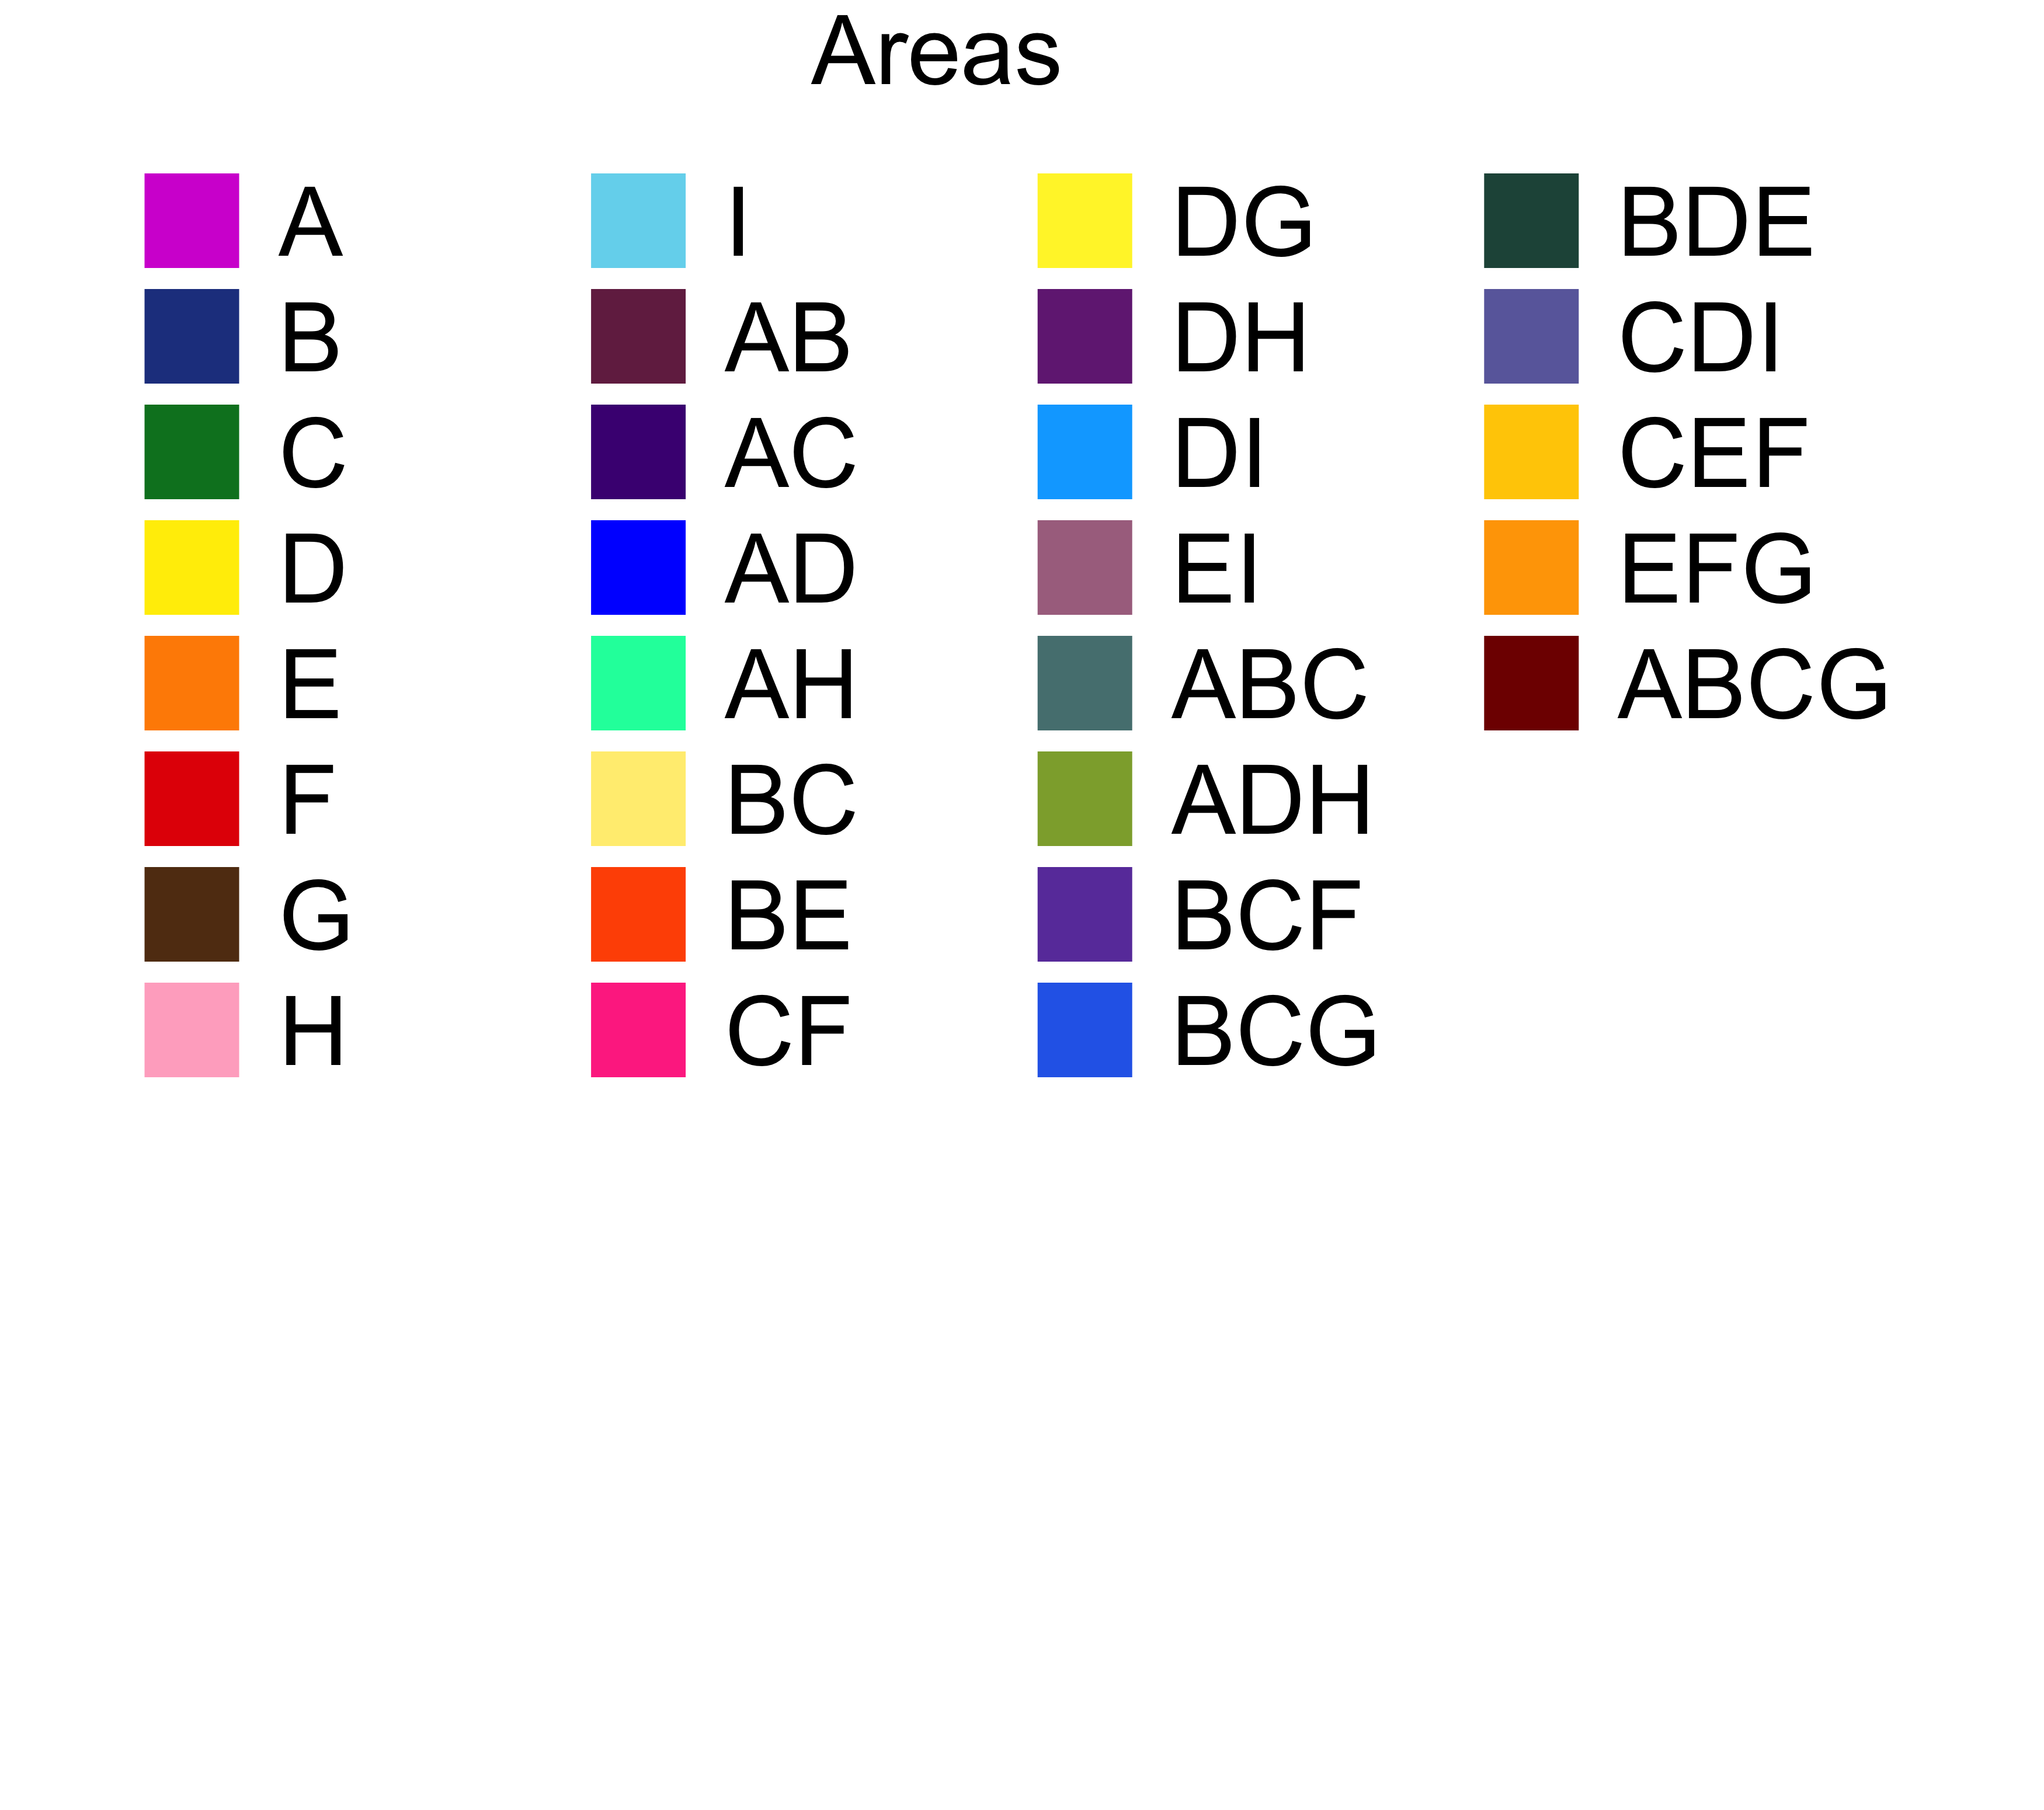
\includegraphics[width = \linewidth]{figures/BGB-legend.png}
  \caption{Legend for plots.}
  \label{fig-legend}
\end{figure} 

%-----------------------------------------------------------------------------------
\subsubsection{All pinnipeds}

% figure
\begin{figure}[H]
 \centering
  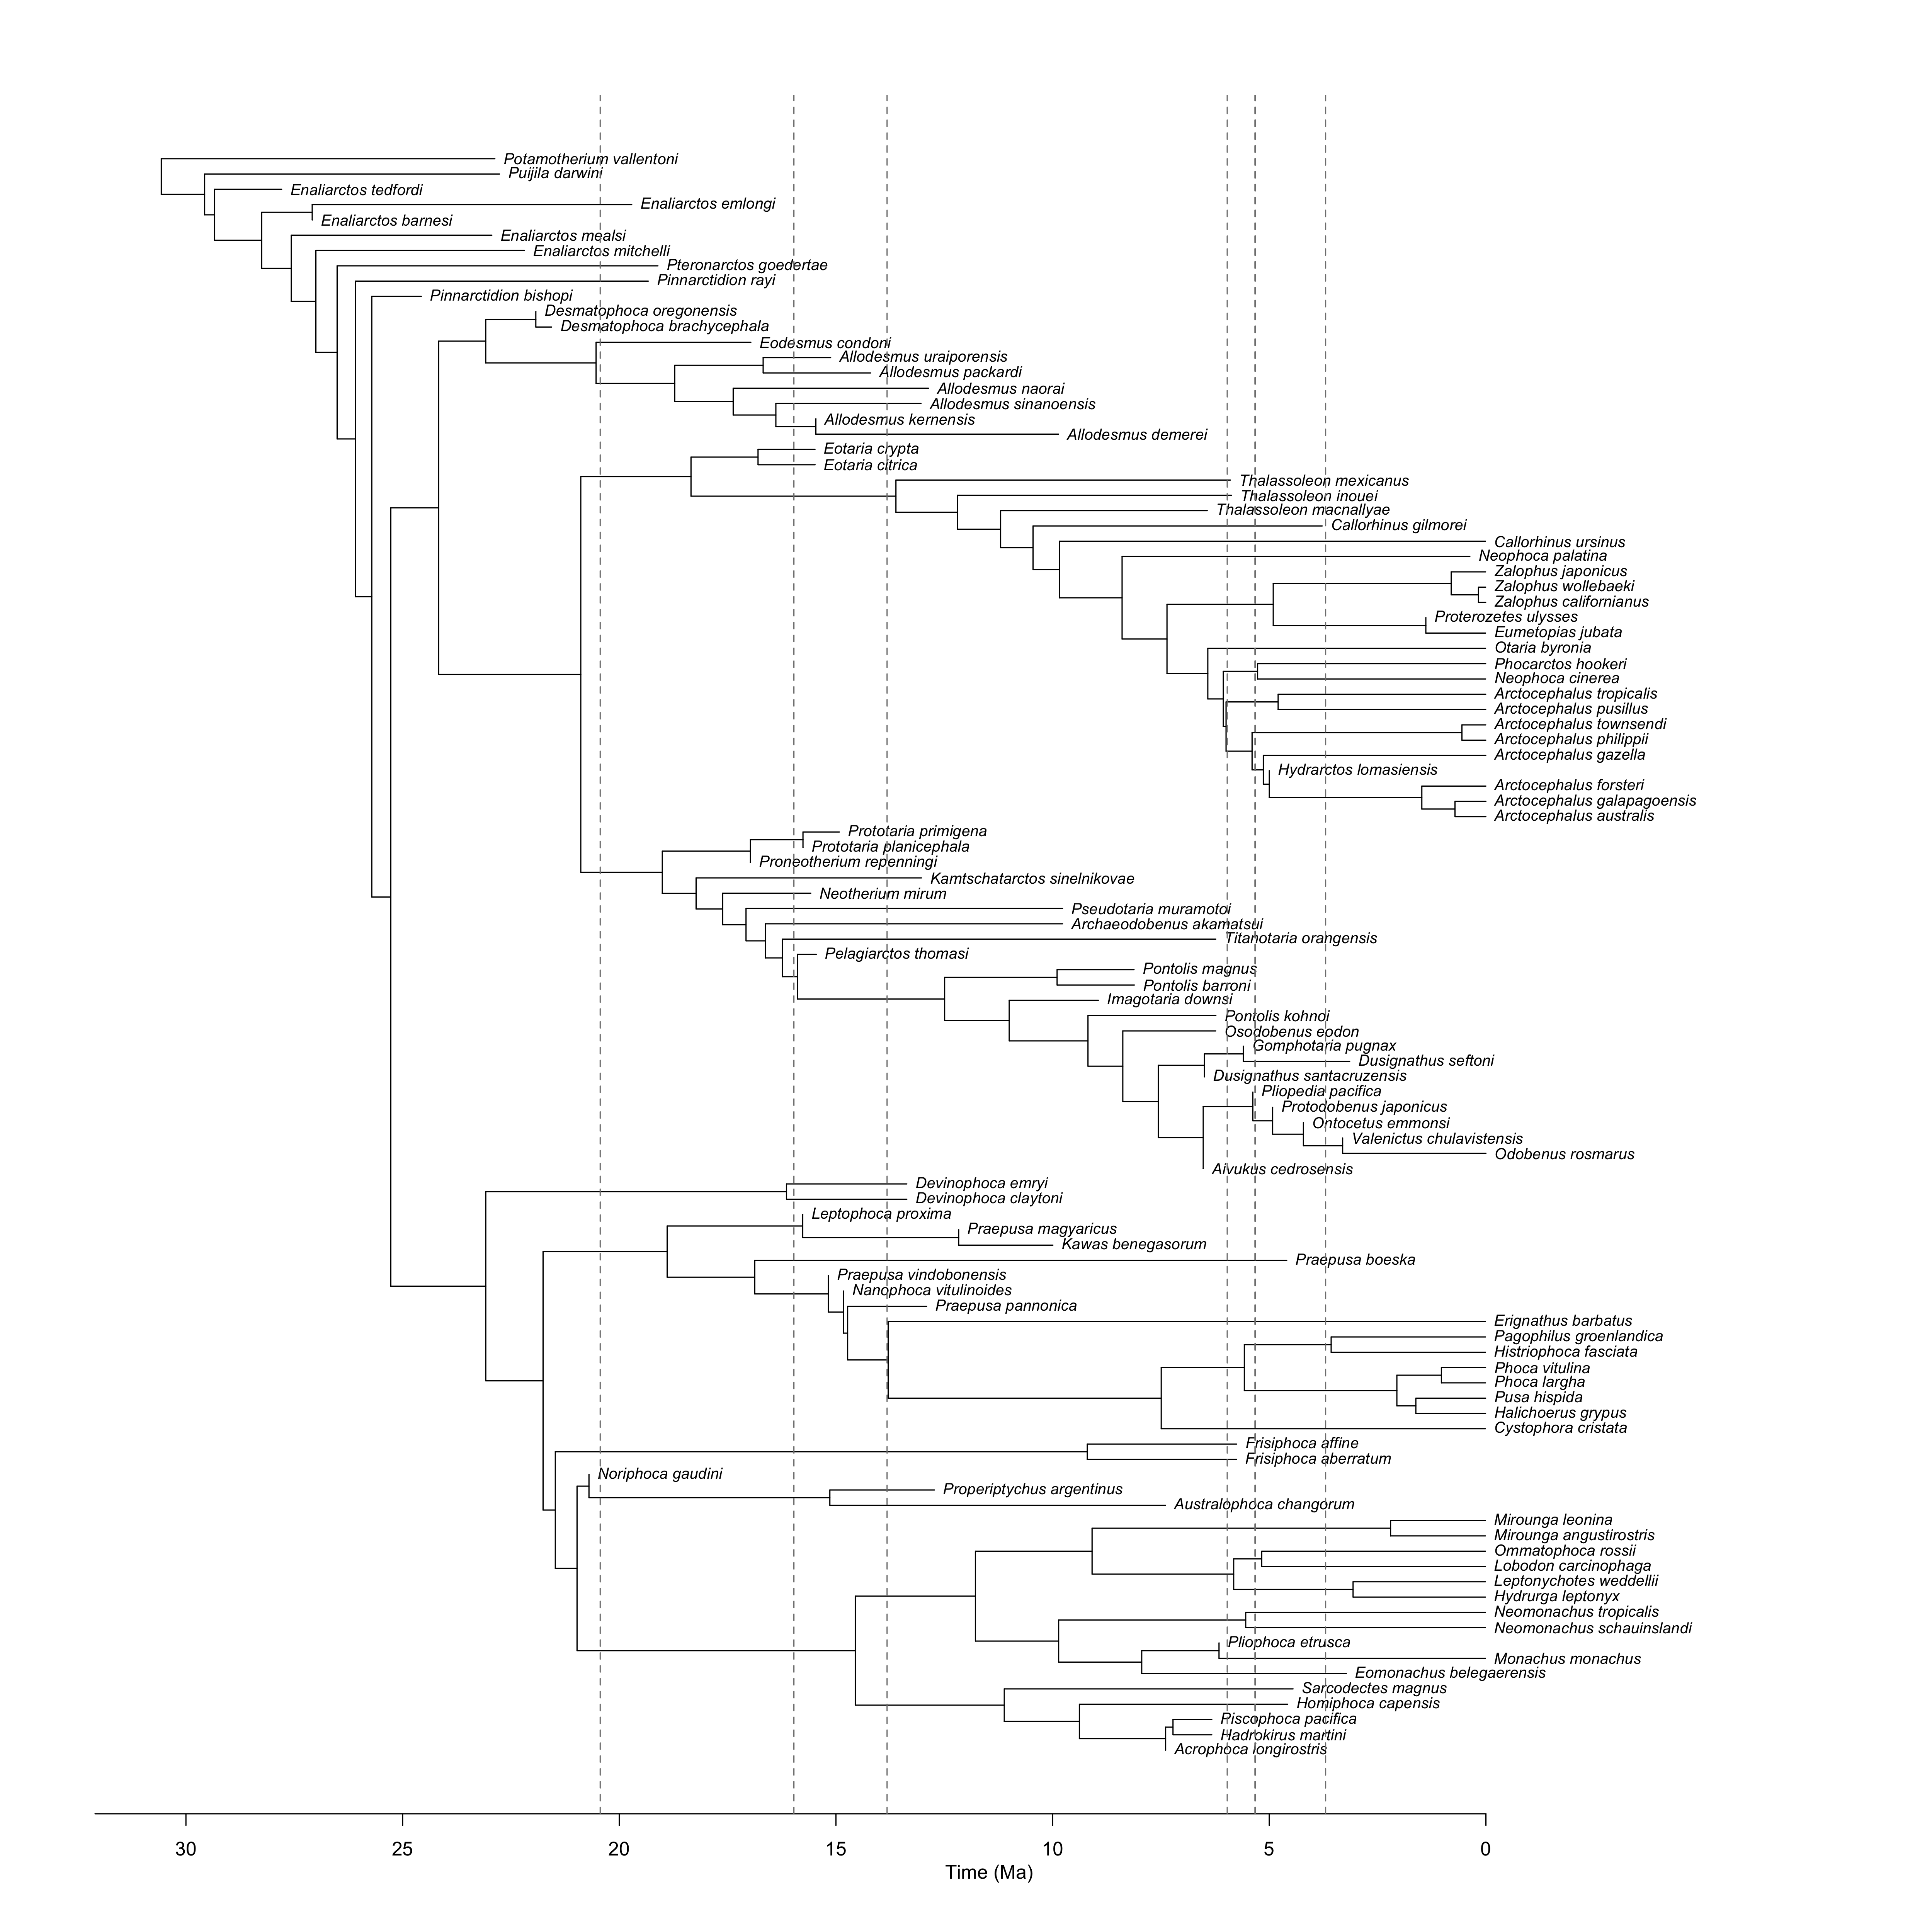
\includegraphics[width = \linewidth]{figures/all-pinnipeds-tree.png}
  \caption{Phylogeny of all pinnipeds with taxon names to aid understanding of the following results which have taxon names removed to improve readability.}
  \label{fig-all-tree}
\end{figure} 

% figure
\begin{figure}[H]
 \centering
  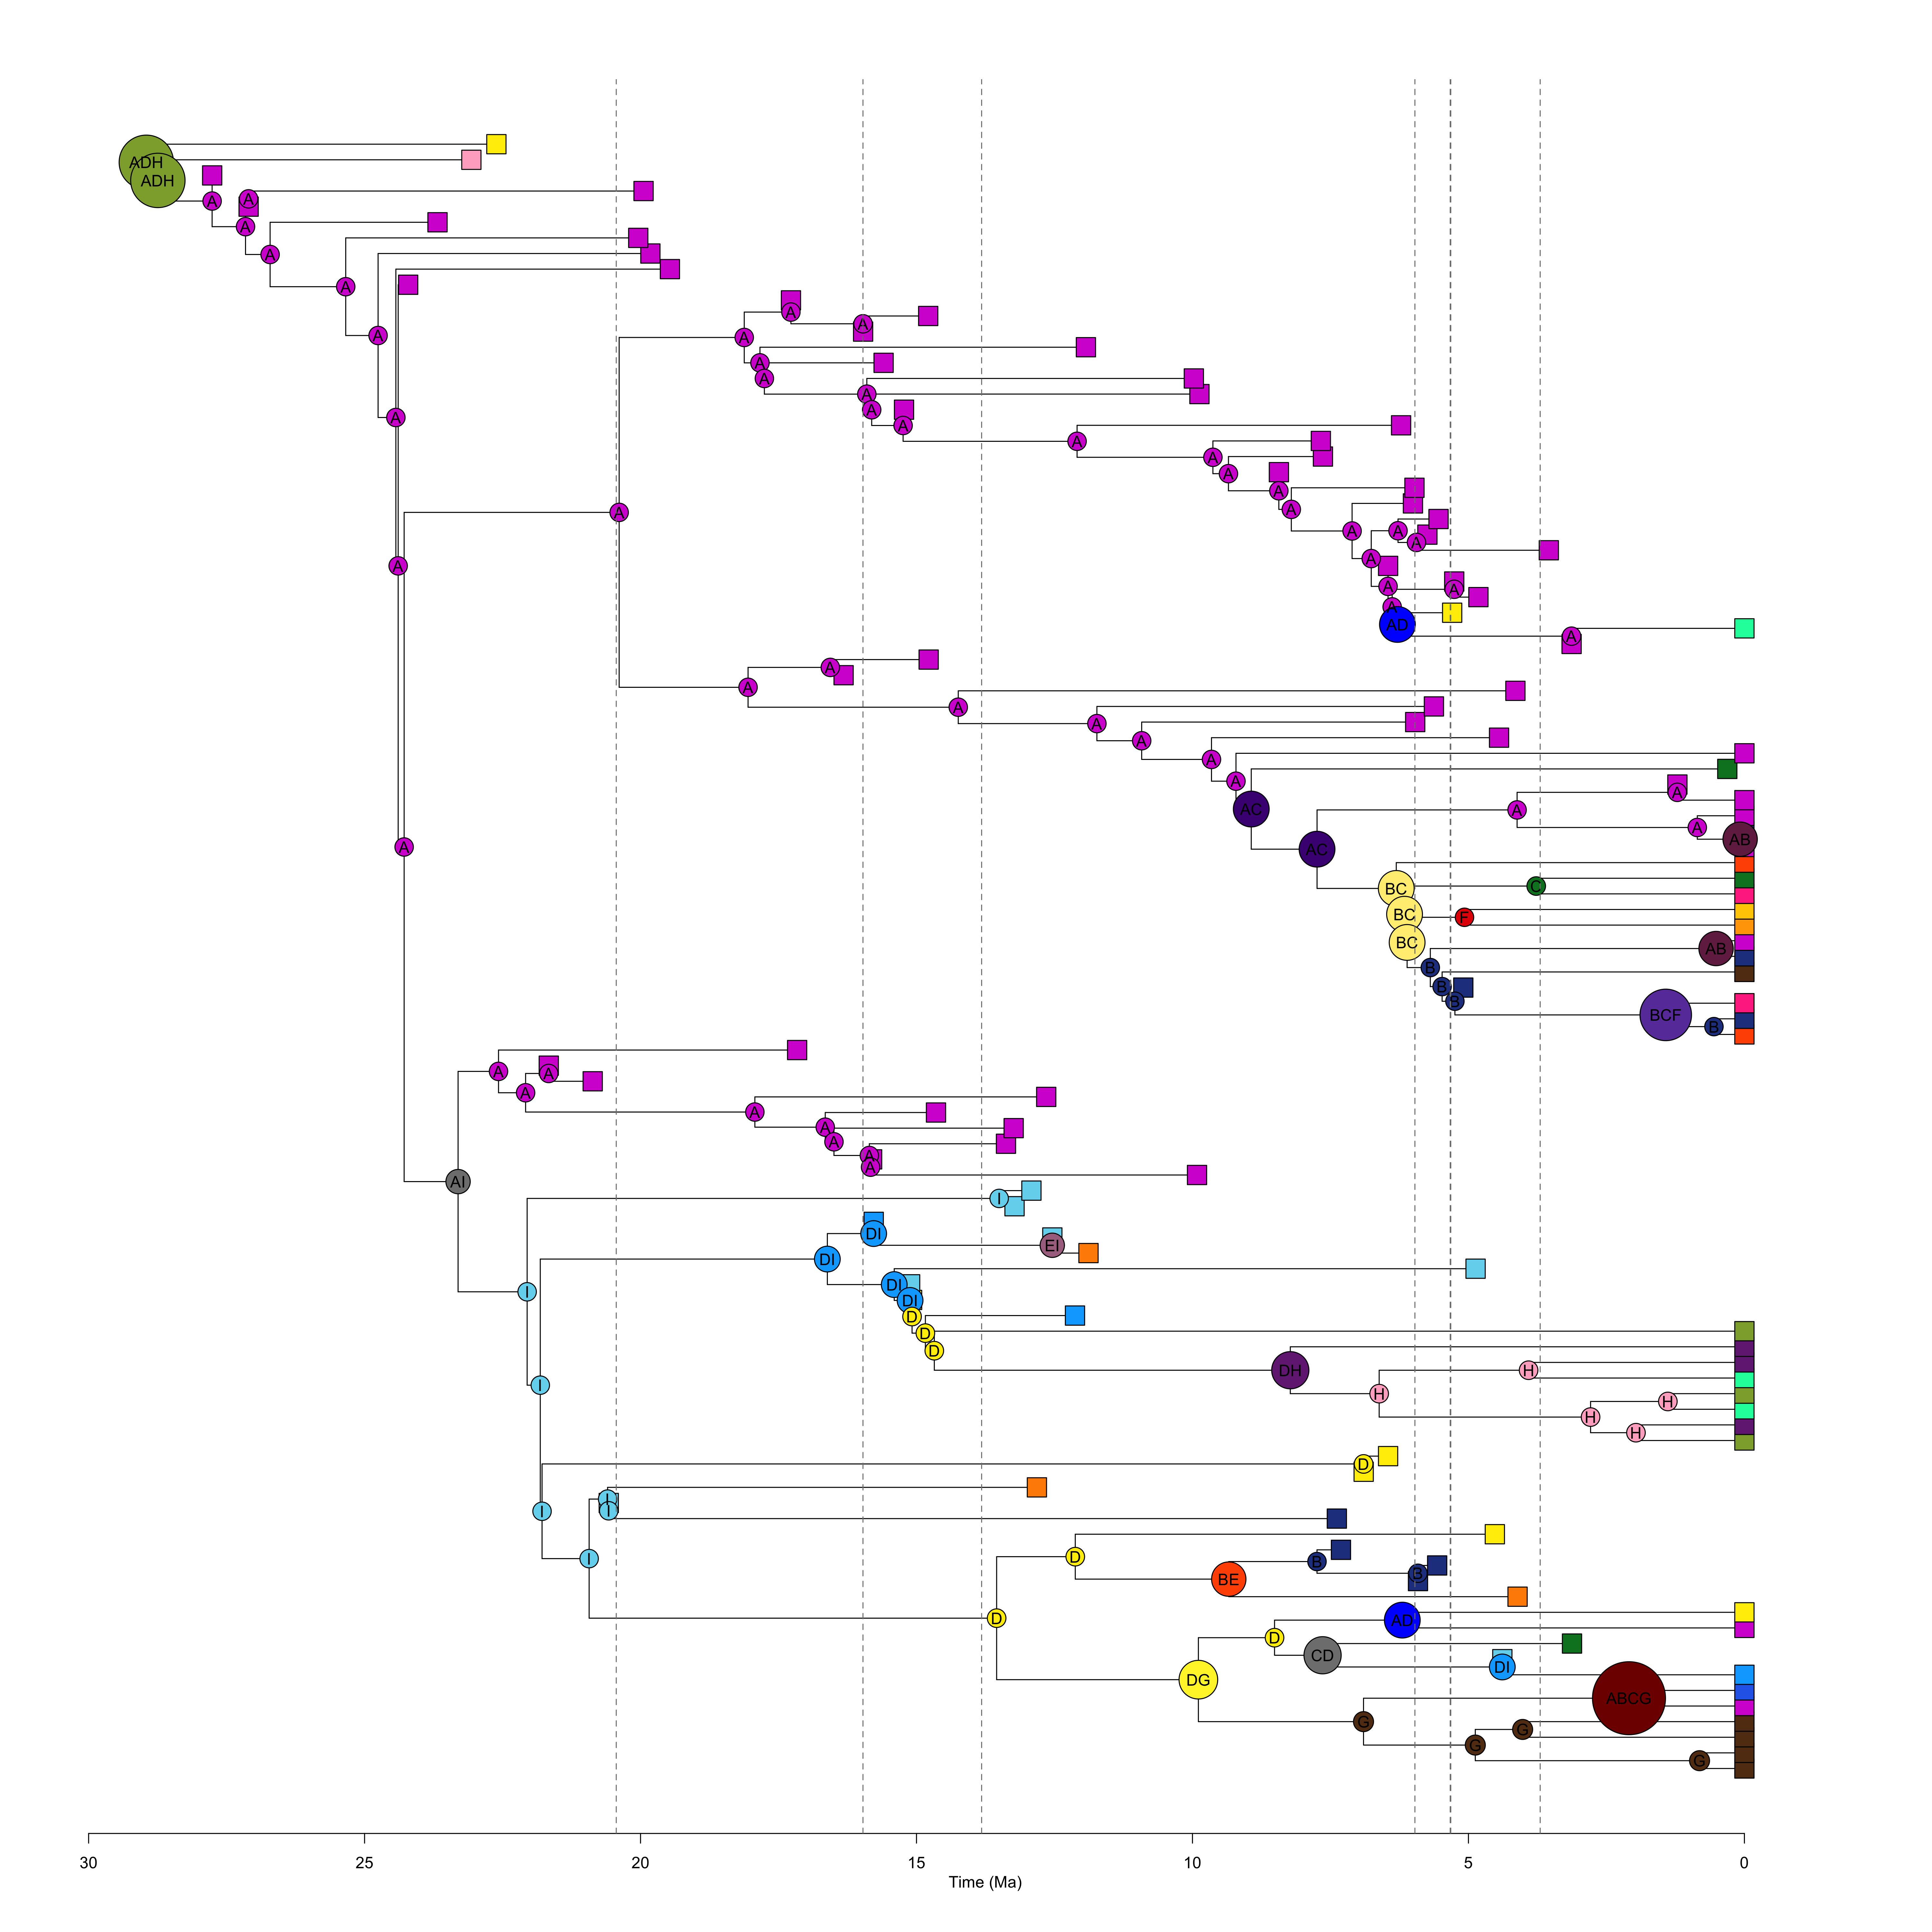
\includegraphics[width = \linewidth]{figures/all-pinnipeds-DEC-impossible-MLstates.png}
  \caption{All pinnipeds, DEC model, impossible states removed. Nodes show Maximum Likelihood states.}
  \label{fig-all-dec-ml}
\end{figure} 

% figure
\begin{figure}[H]
 \centering
  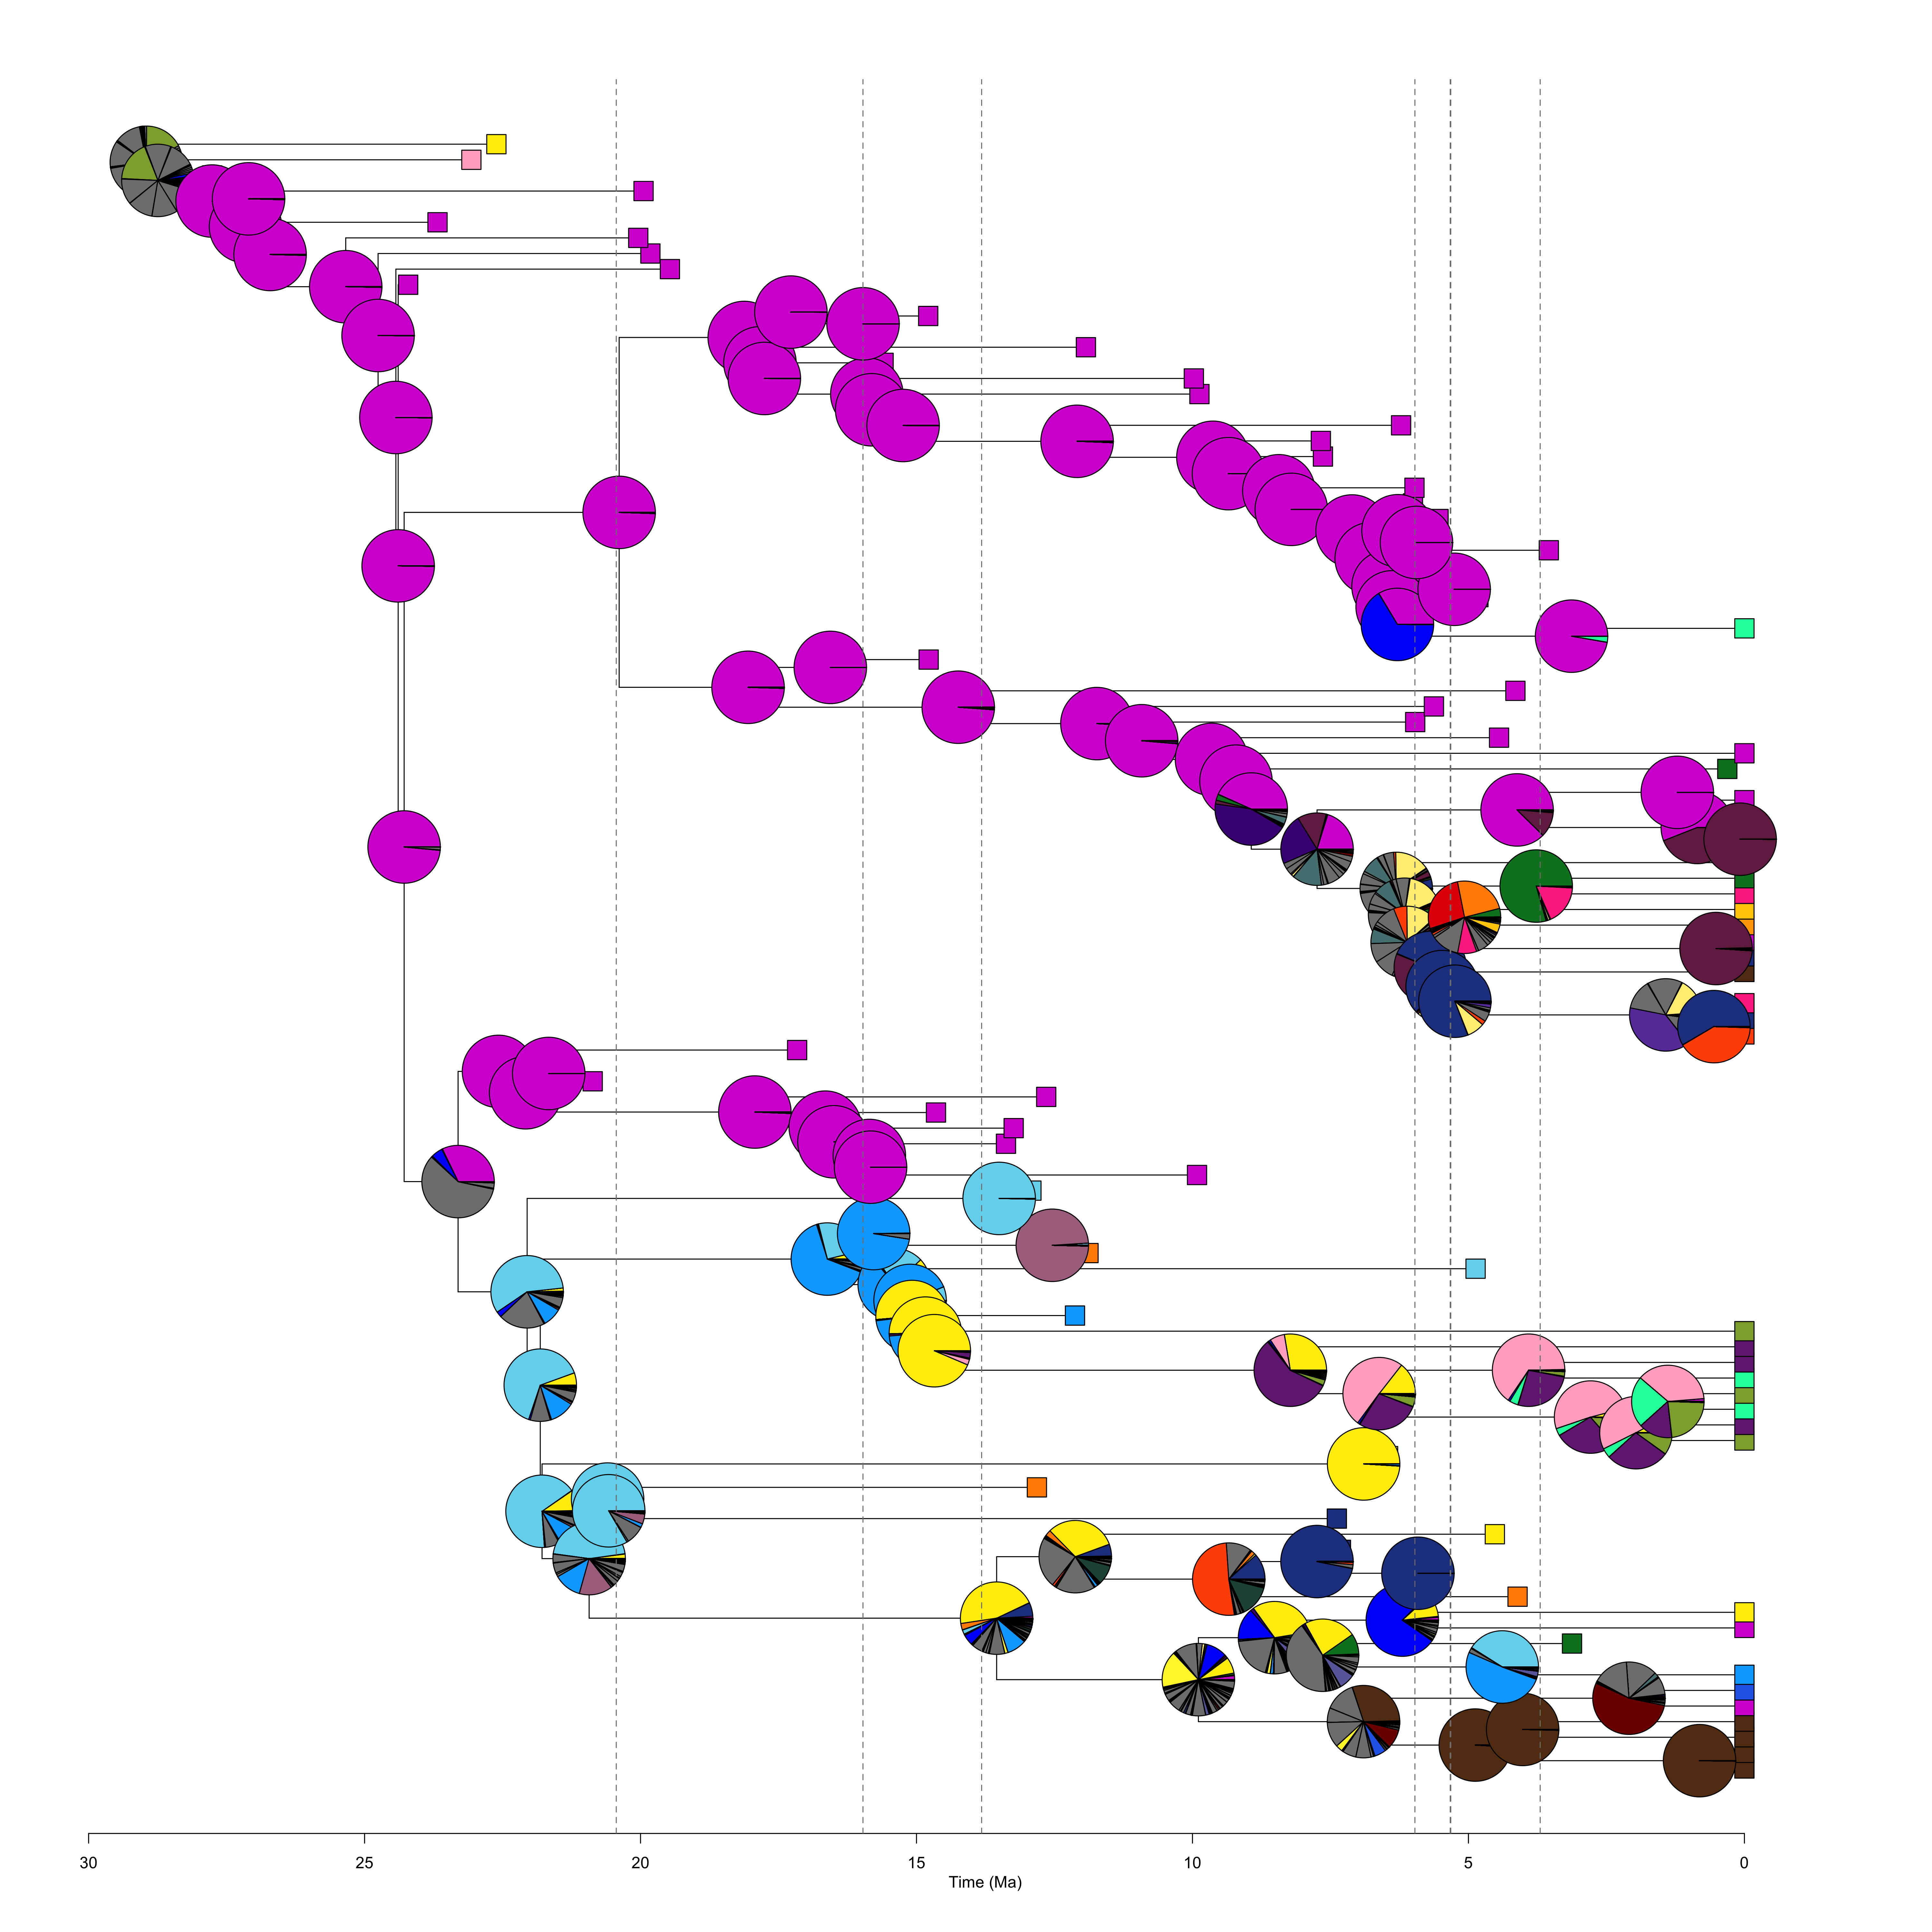
\includegraphics[width = \linewidth]{figures/all-pinnipeds-DEC-impossible-pies.png}
  \caption{All pinnipeds, DEC model, impossible states removed. Nodes show relative probabilities of each state.}
  \label{fig-all-dec-pie}
\end{figure} 

% figure
%\begin{figure}[H]
% \centering
%  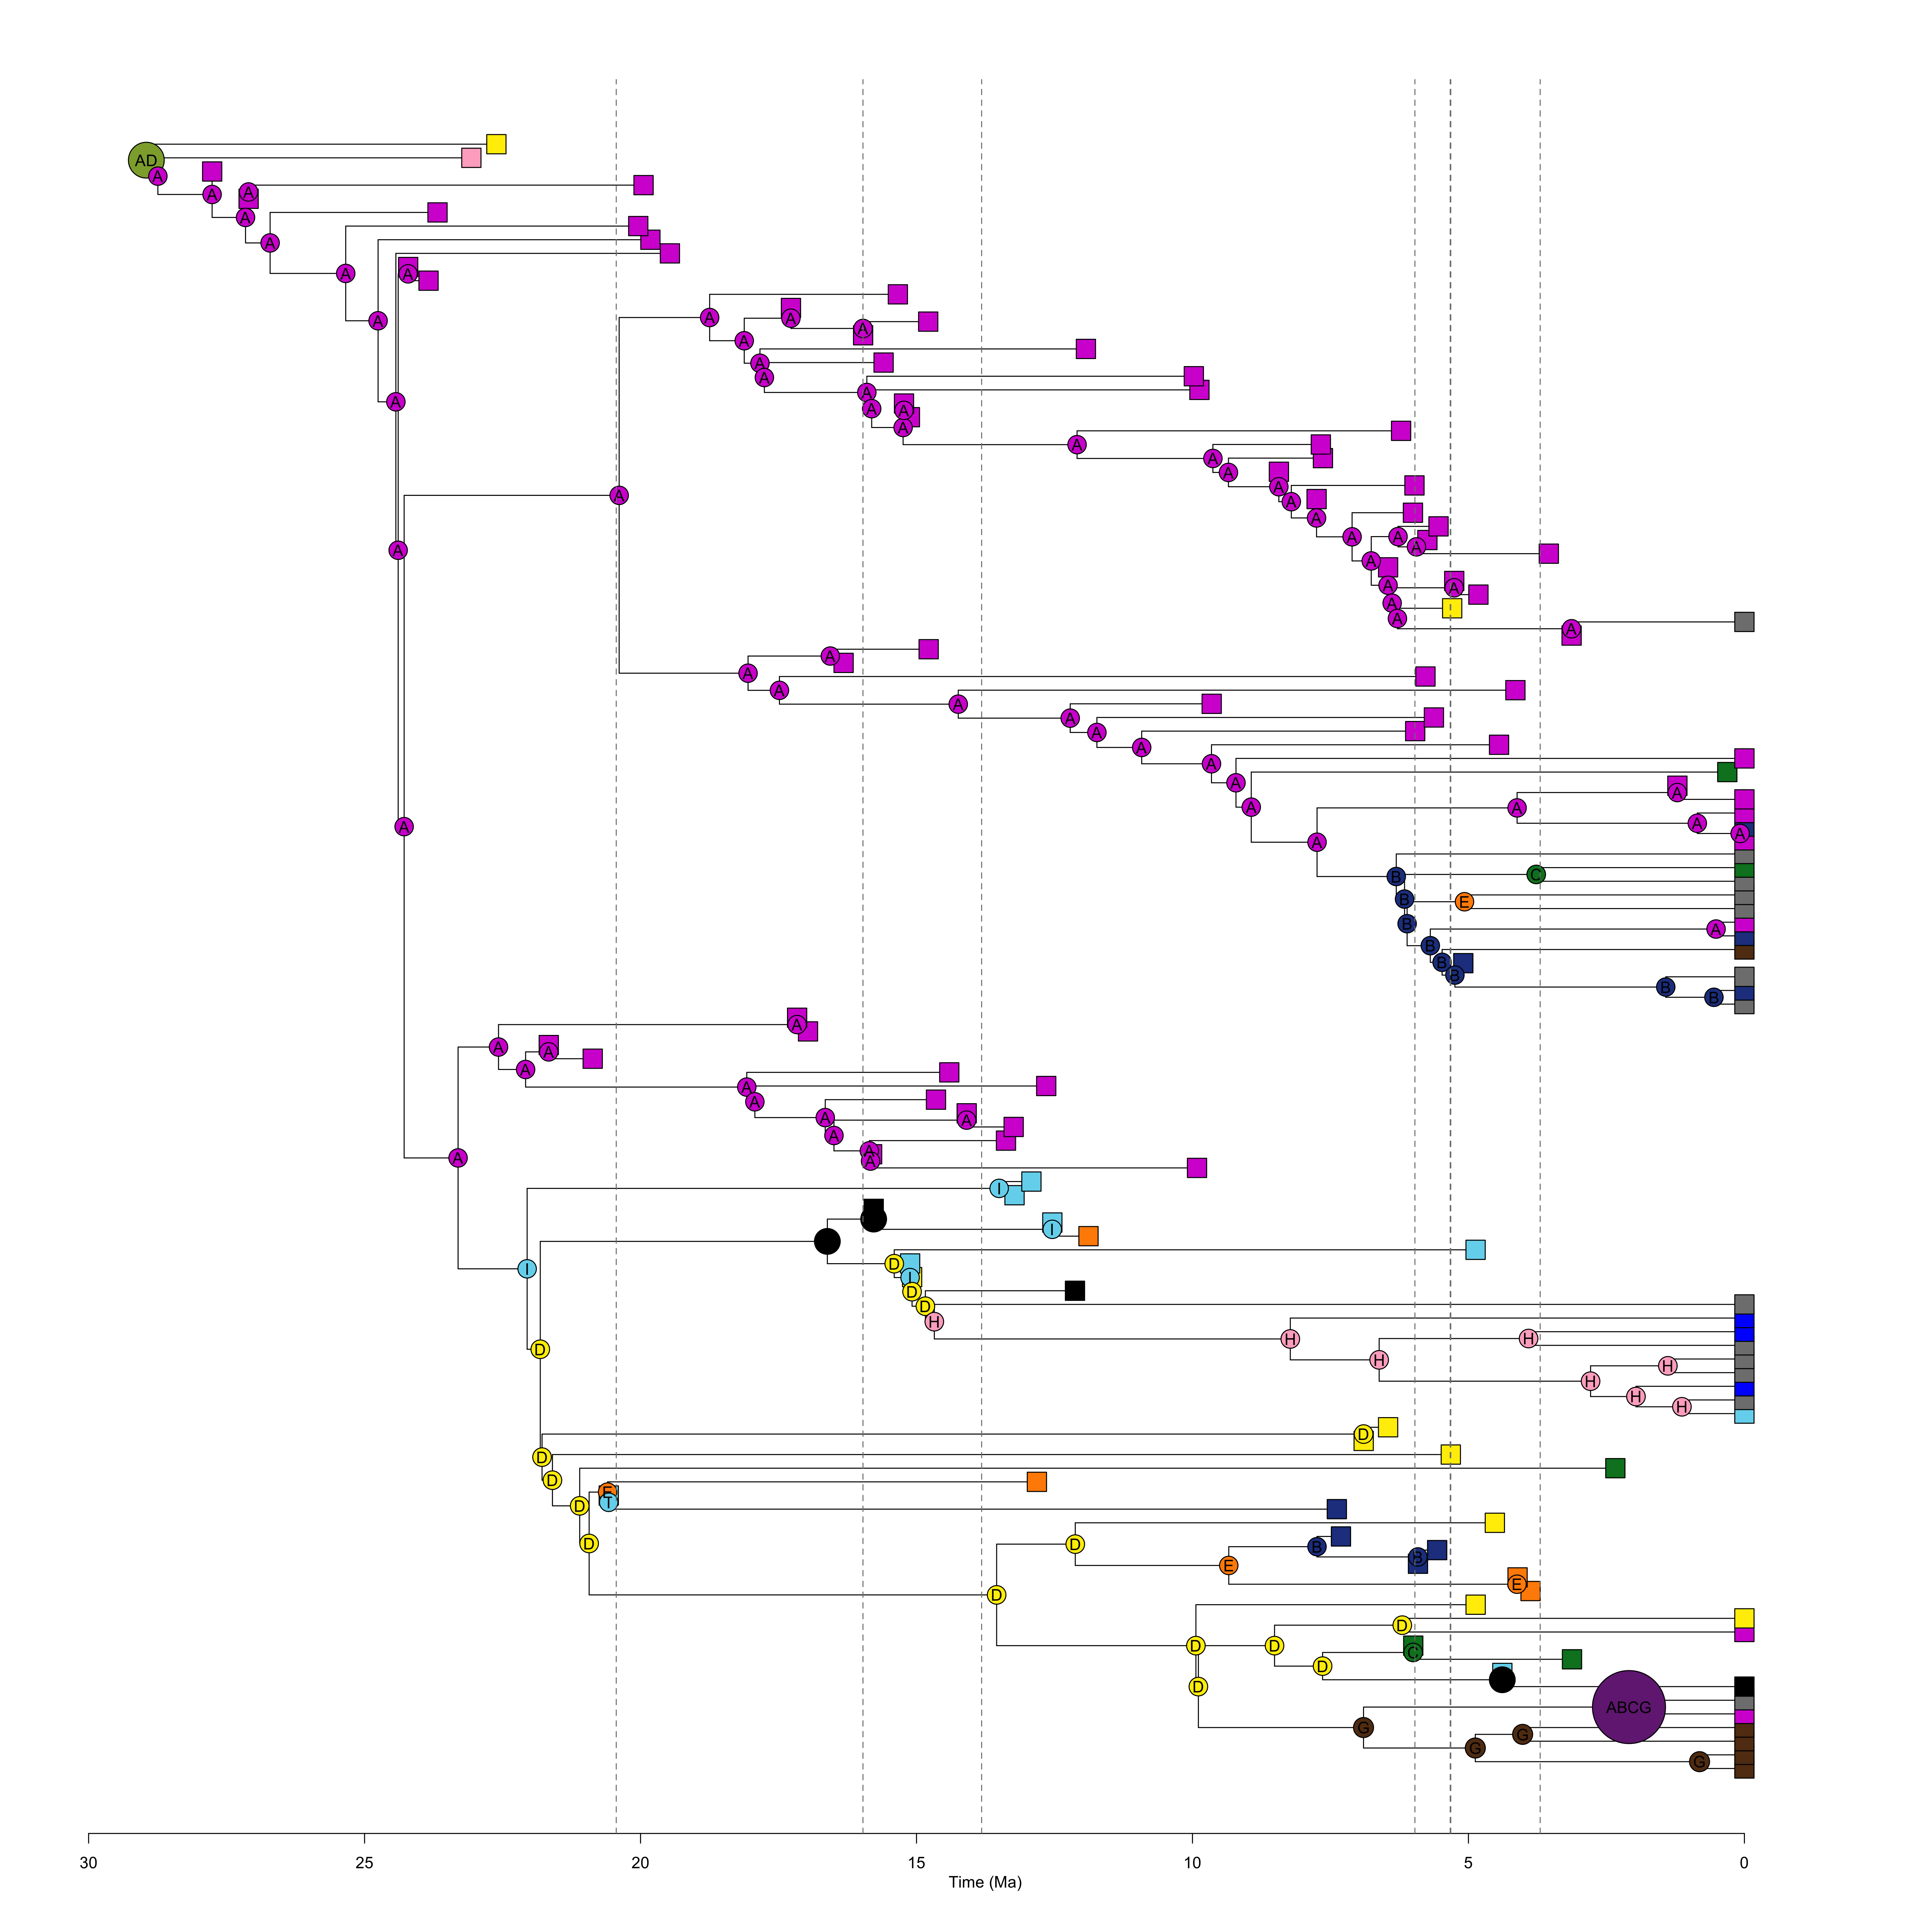
\includegraphics[width = \linewidth]{figures/all-pinnipeds-DECj-impossible-MLstates.png}
%  \caption{All pinnipeds, DEC+J model, impossible states removed. Nodes show Maximum Likelihood states.}
%  \label{fig-all-decj-ml}
%\end{figure} 

% figure
%\begin{figure}[H]
% \centering
%  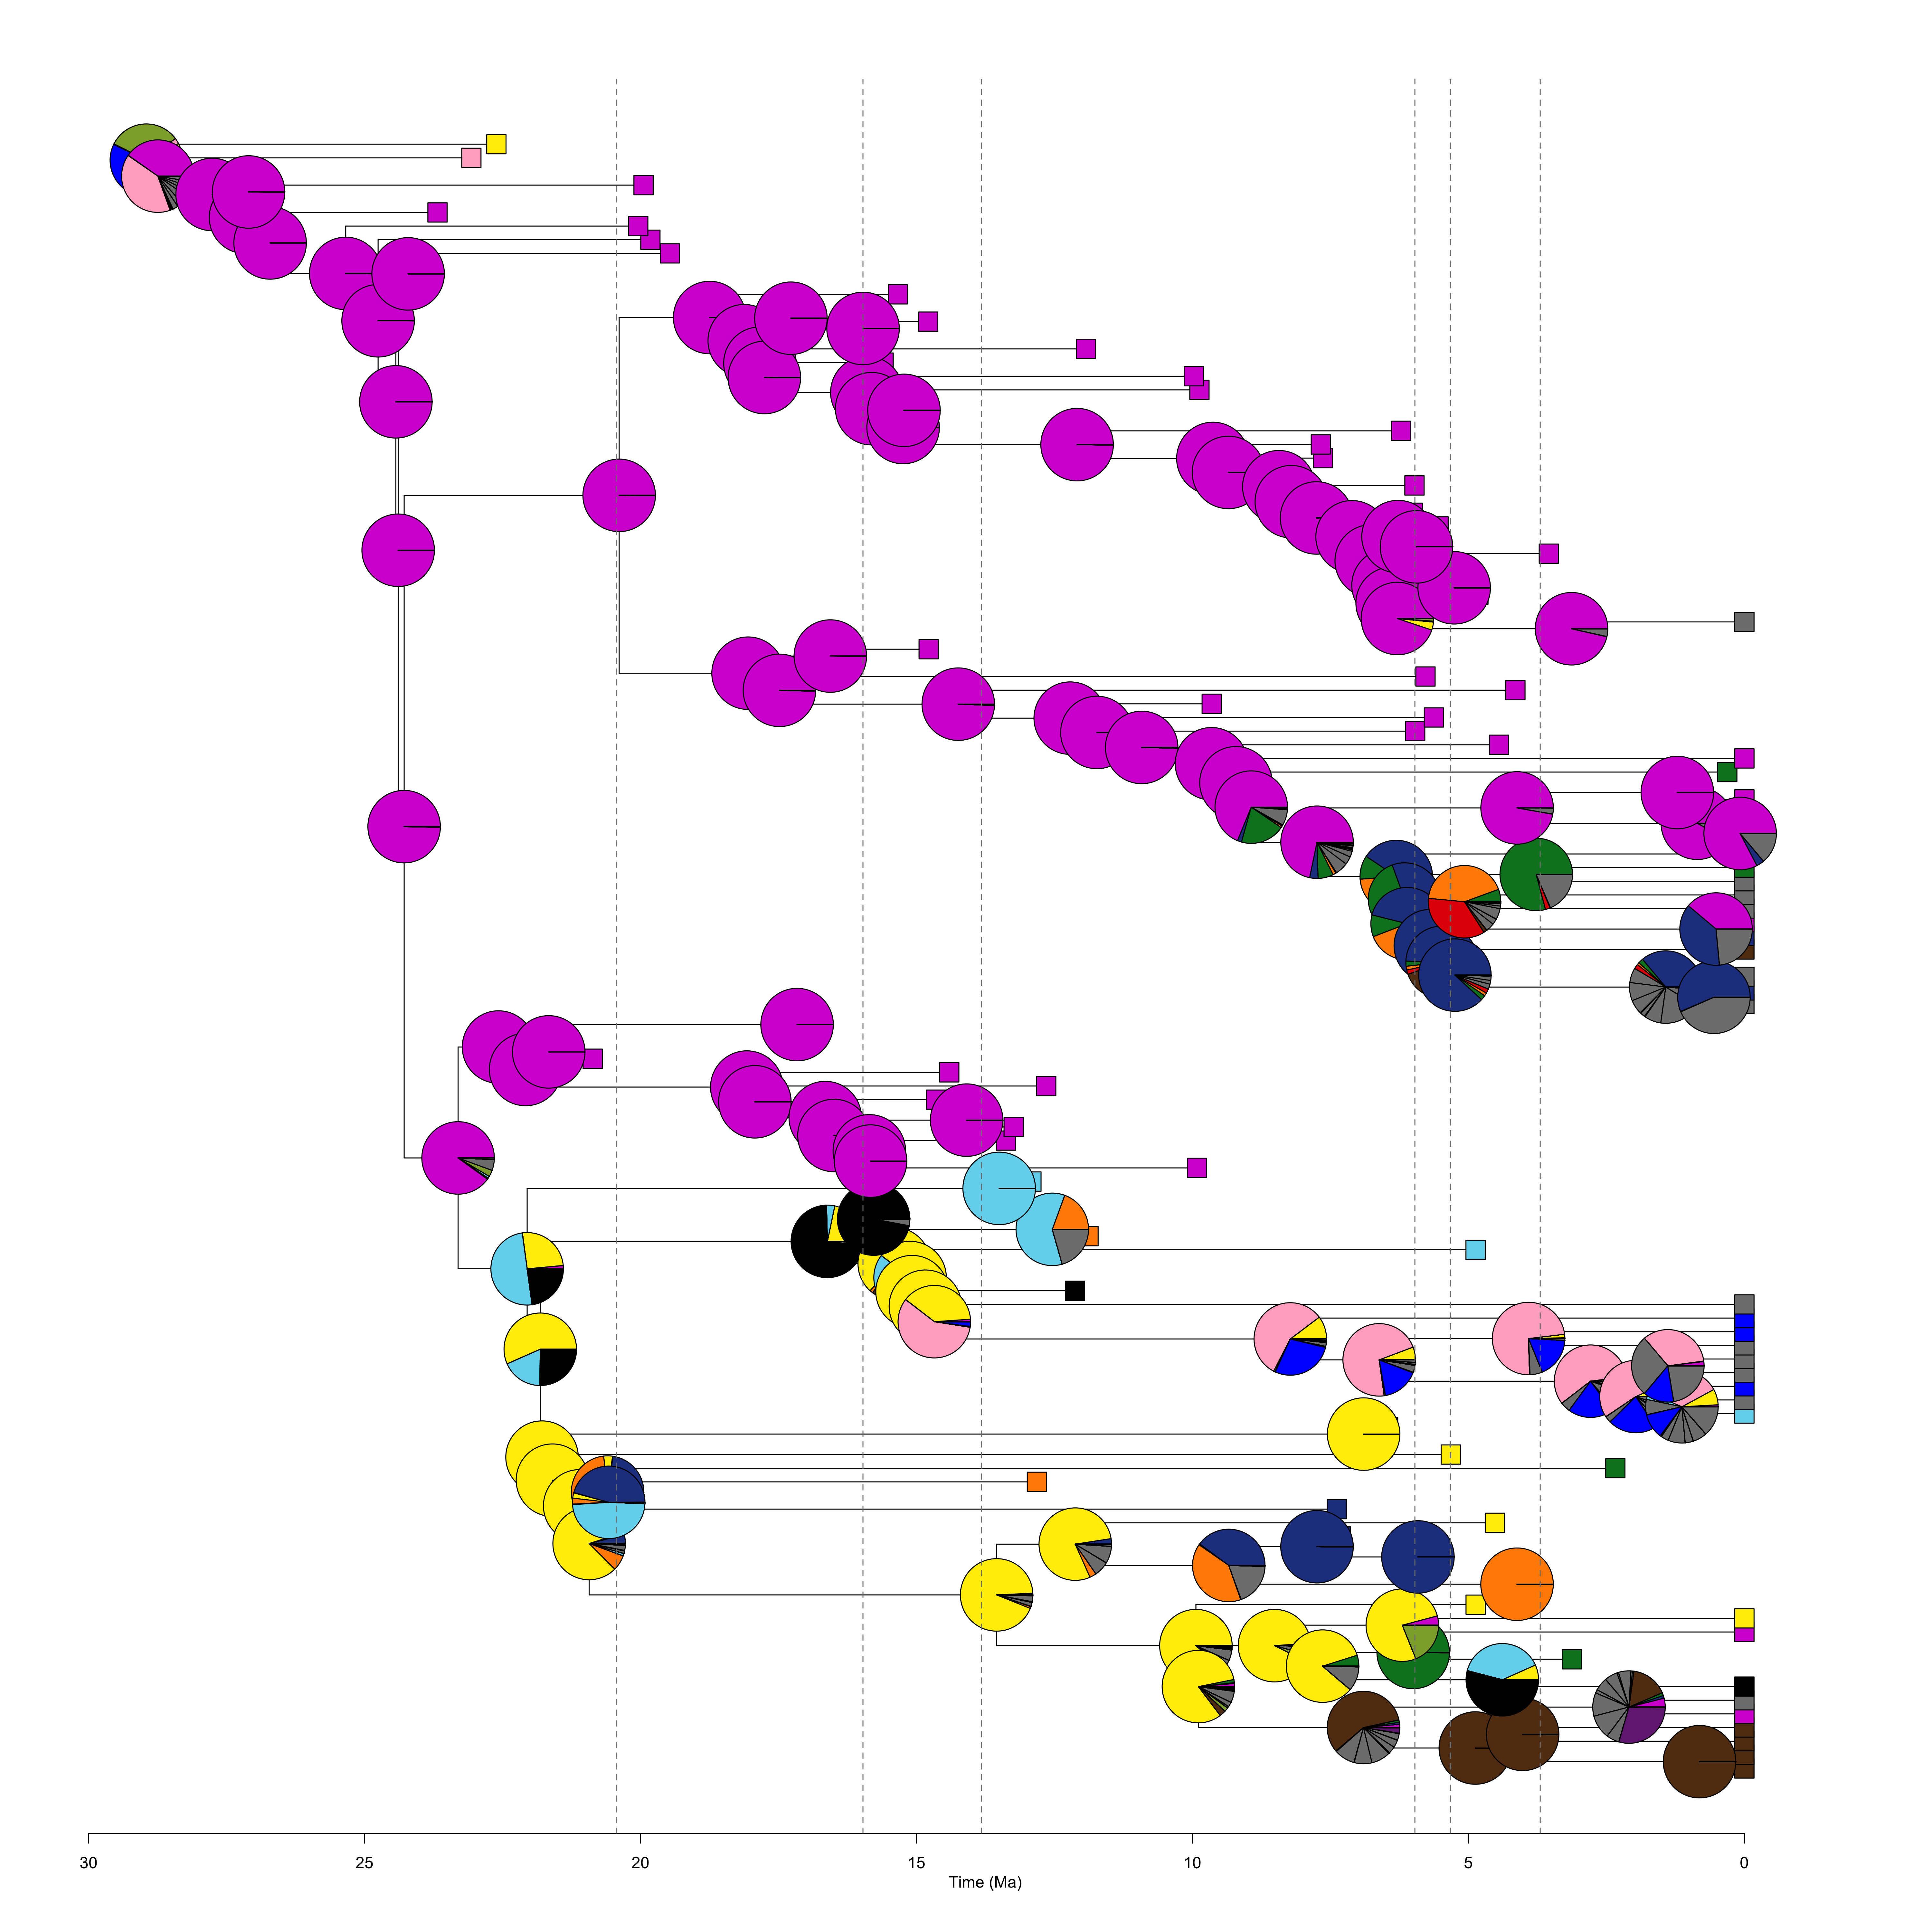
\includegraphics[width = \linewidth]{figures/all-pinnipeds-DECj-impossible-pies.png}
%  \caption{All pinnipeds, DEC+J model, impossible states removed. Nodes show relative probabilities of each state.}
%  \label{fig-all-decj-pie}
%\end{figure} 
 
%-----------------------------------------------------------------------------------
% unlikely

% figure
%\begin{figure}[H]
% \centering
%  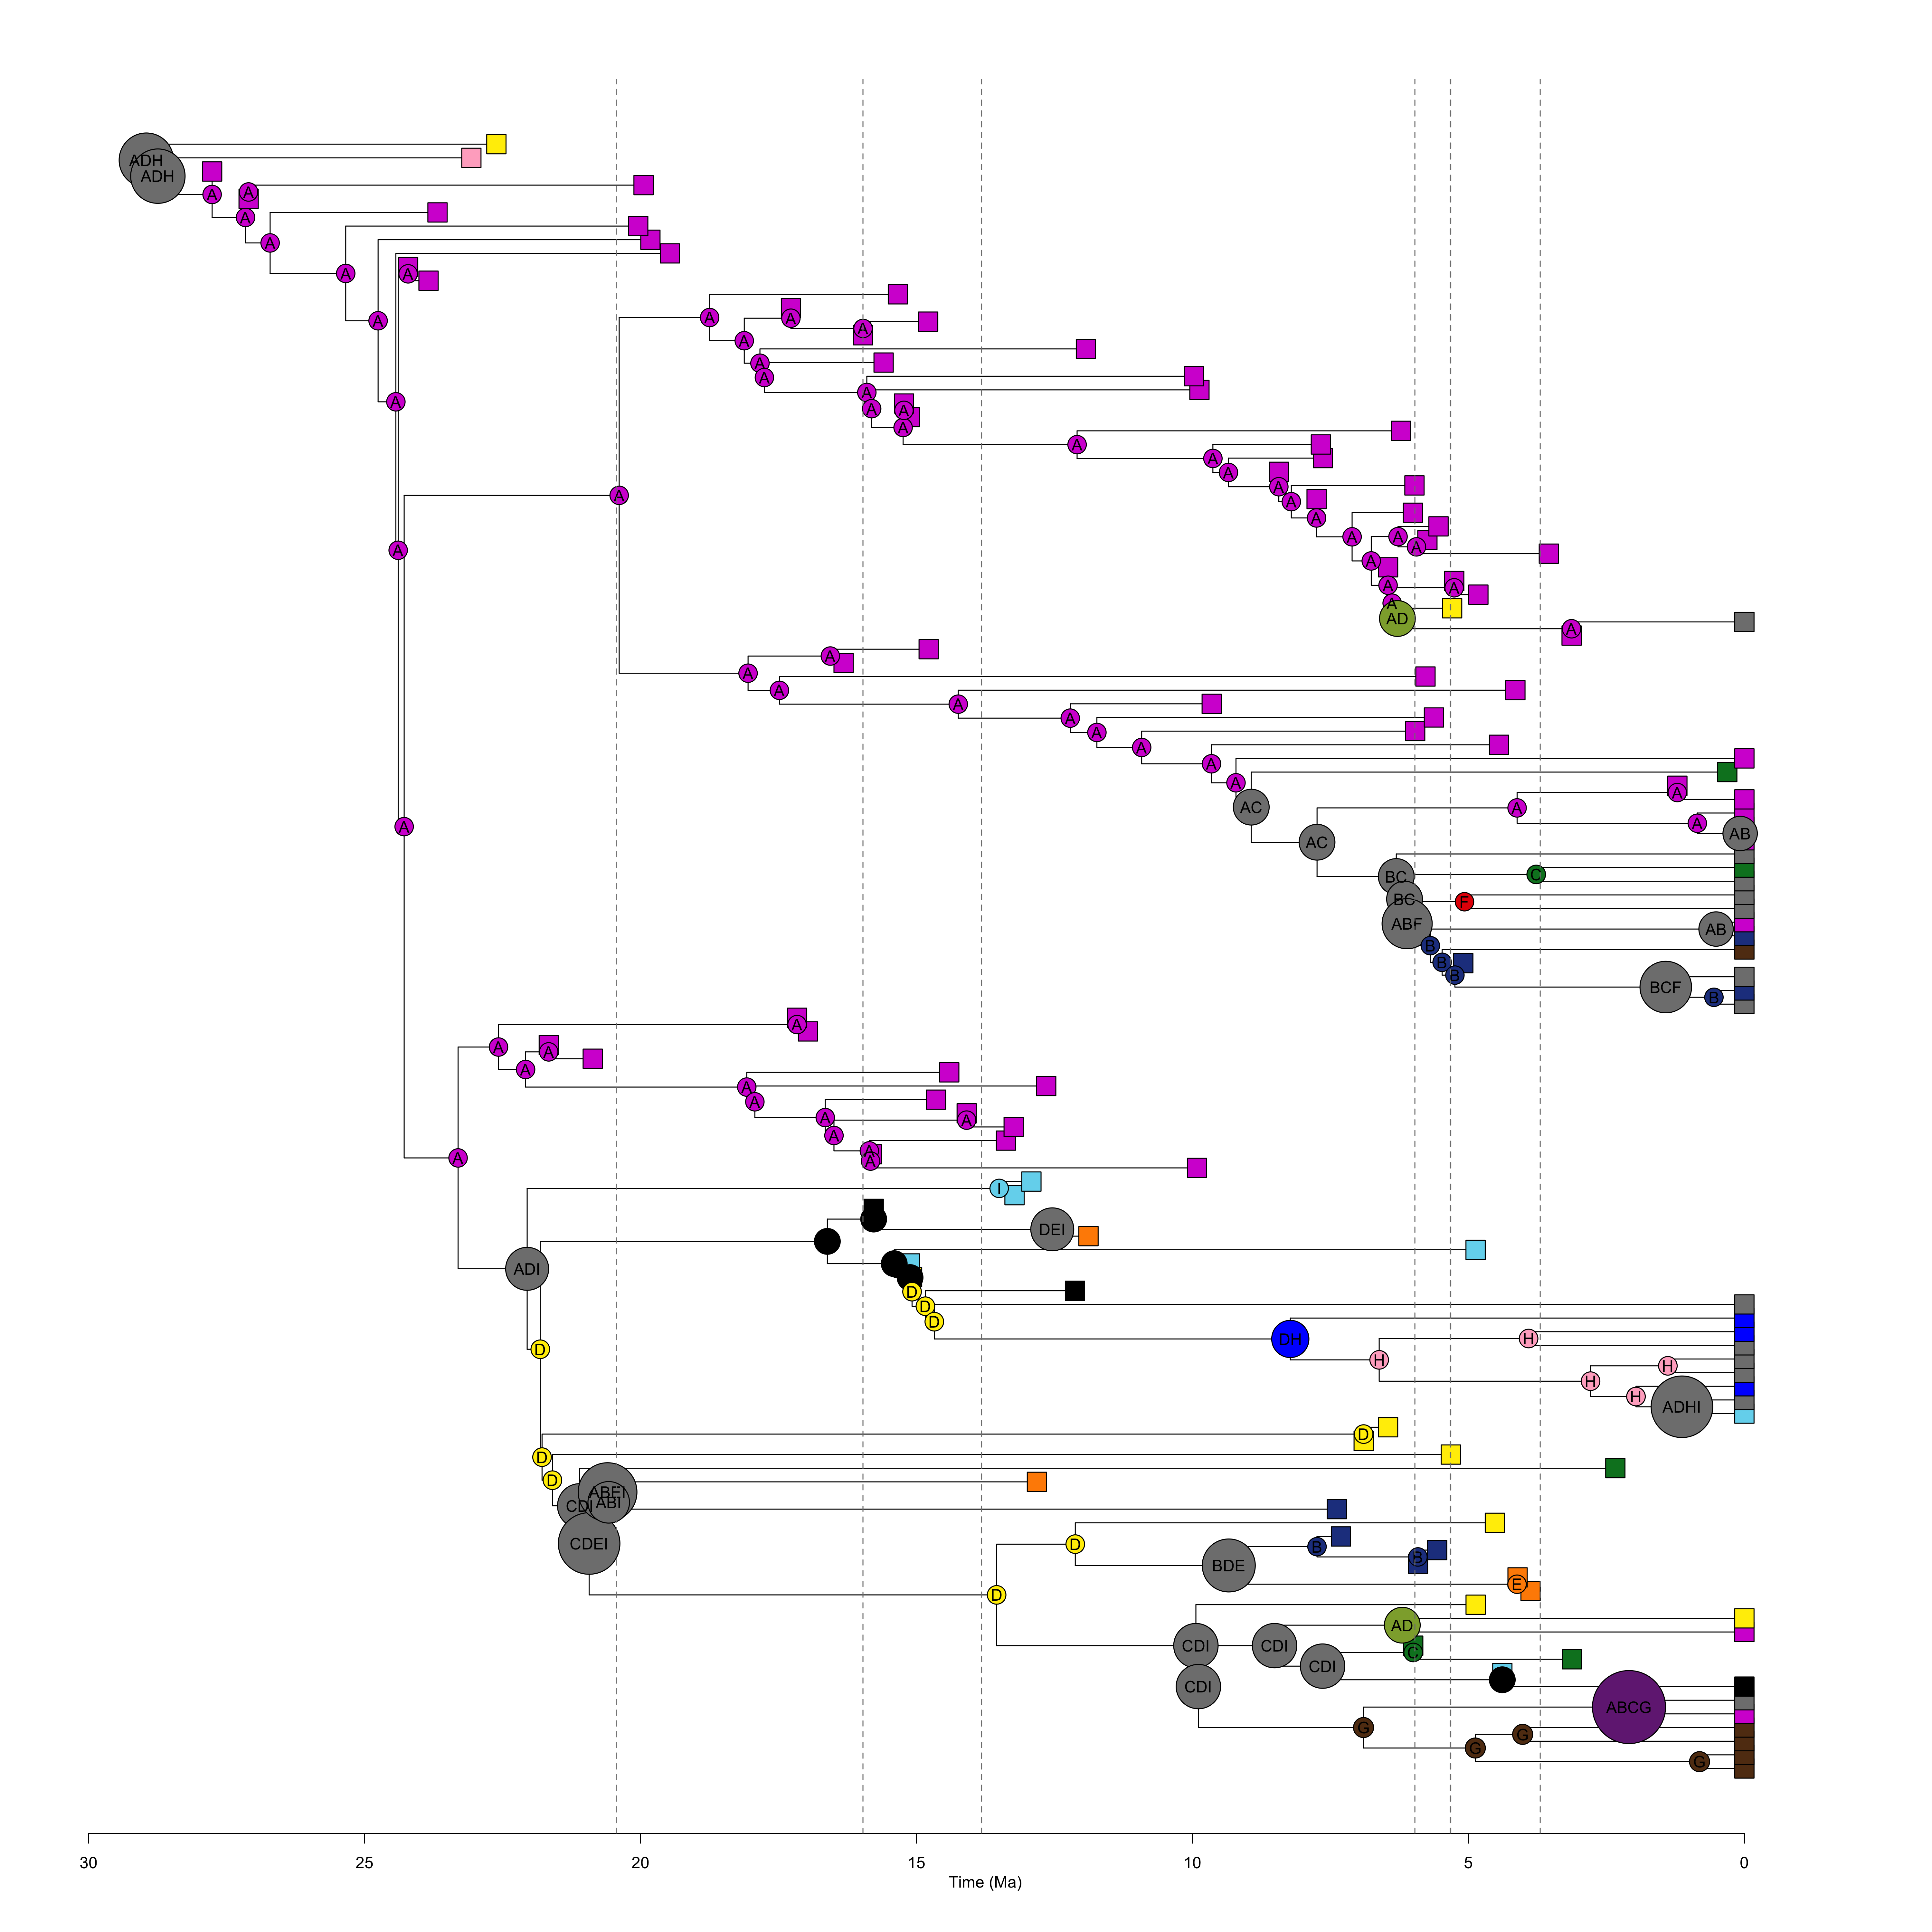
\includegraphics[width = \linewidth]{figures/all-pinnipeds-DEC-unlikely-MLstates.png}
%  \caption{All pinnipeds, DEC model, impossible and unlikely states removed. Nodes show Maximum Likelihood states.}
%  \label{fig-all-dec-ml-unlikely}
%\end{figure} 

% figure
%\begin{figure}[H]
% \centering
%  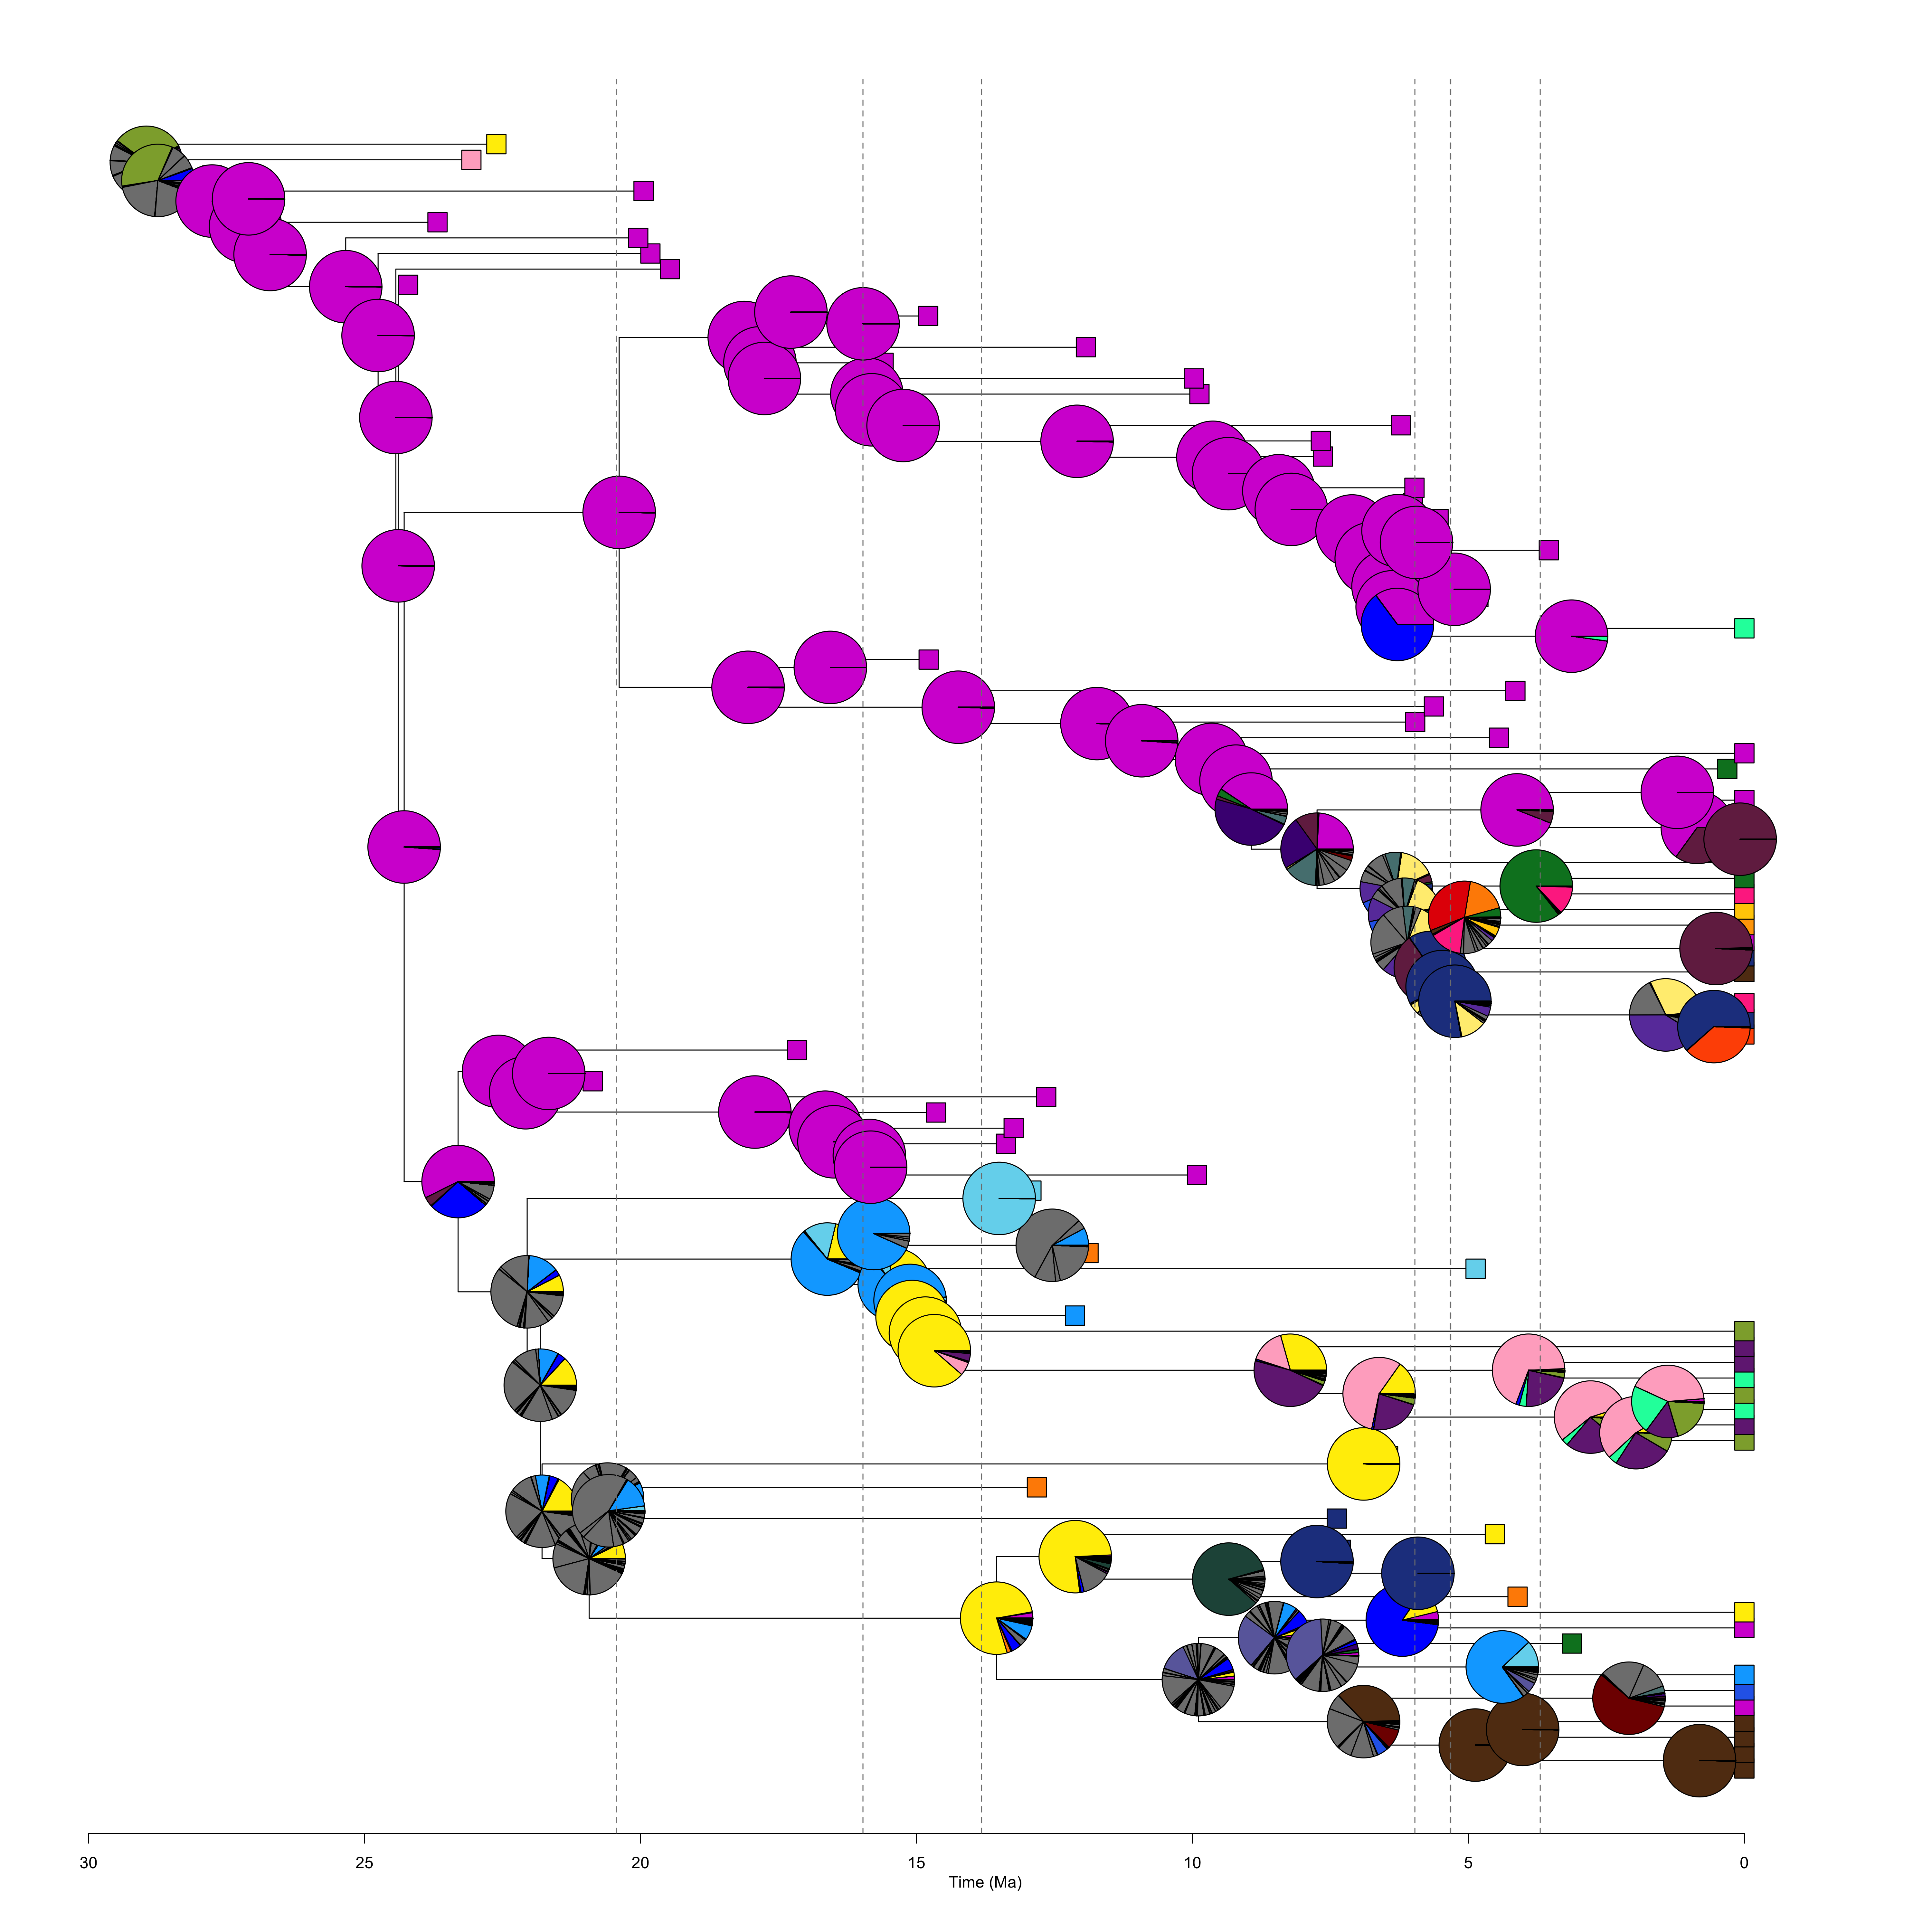
\includegraphics[width = \linewidth]{figures/all-pinnipeds-DEC-unlikely-pies.png}
%  \caption{All pinnipeds, DEC model, impossible and unlikely states removed. Nodes show relative probabilities of each state.}
%  \label{fig-all-dec-pie-unlikely}
%\end{figure} 

% figure
%\begin{figure}[H]
% \centering
%  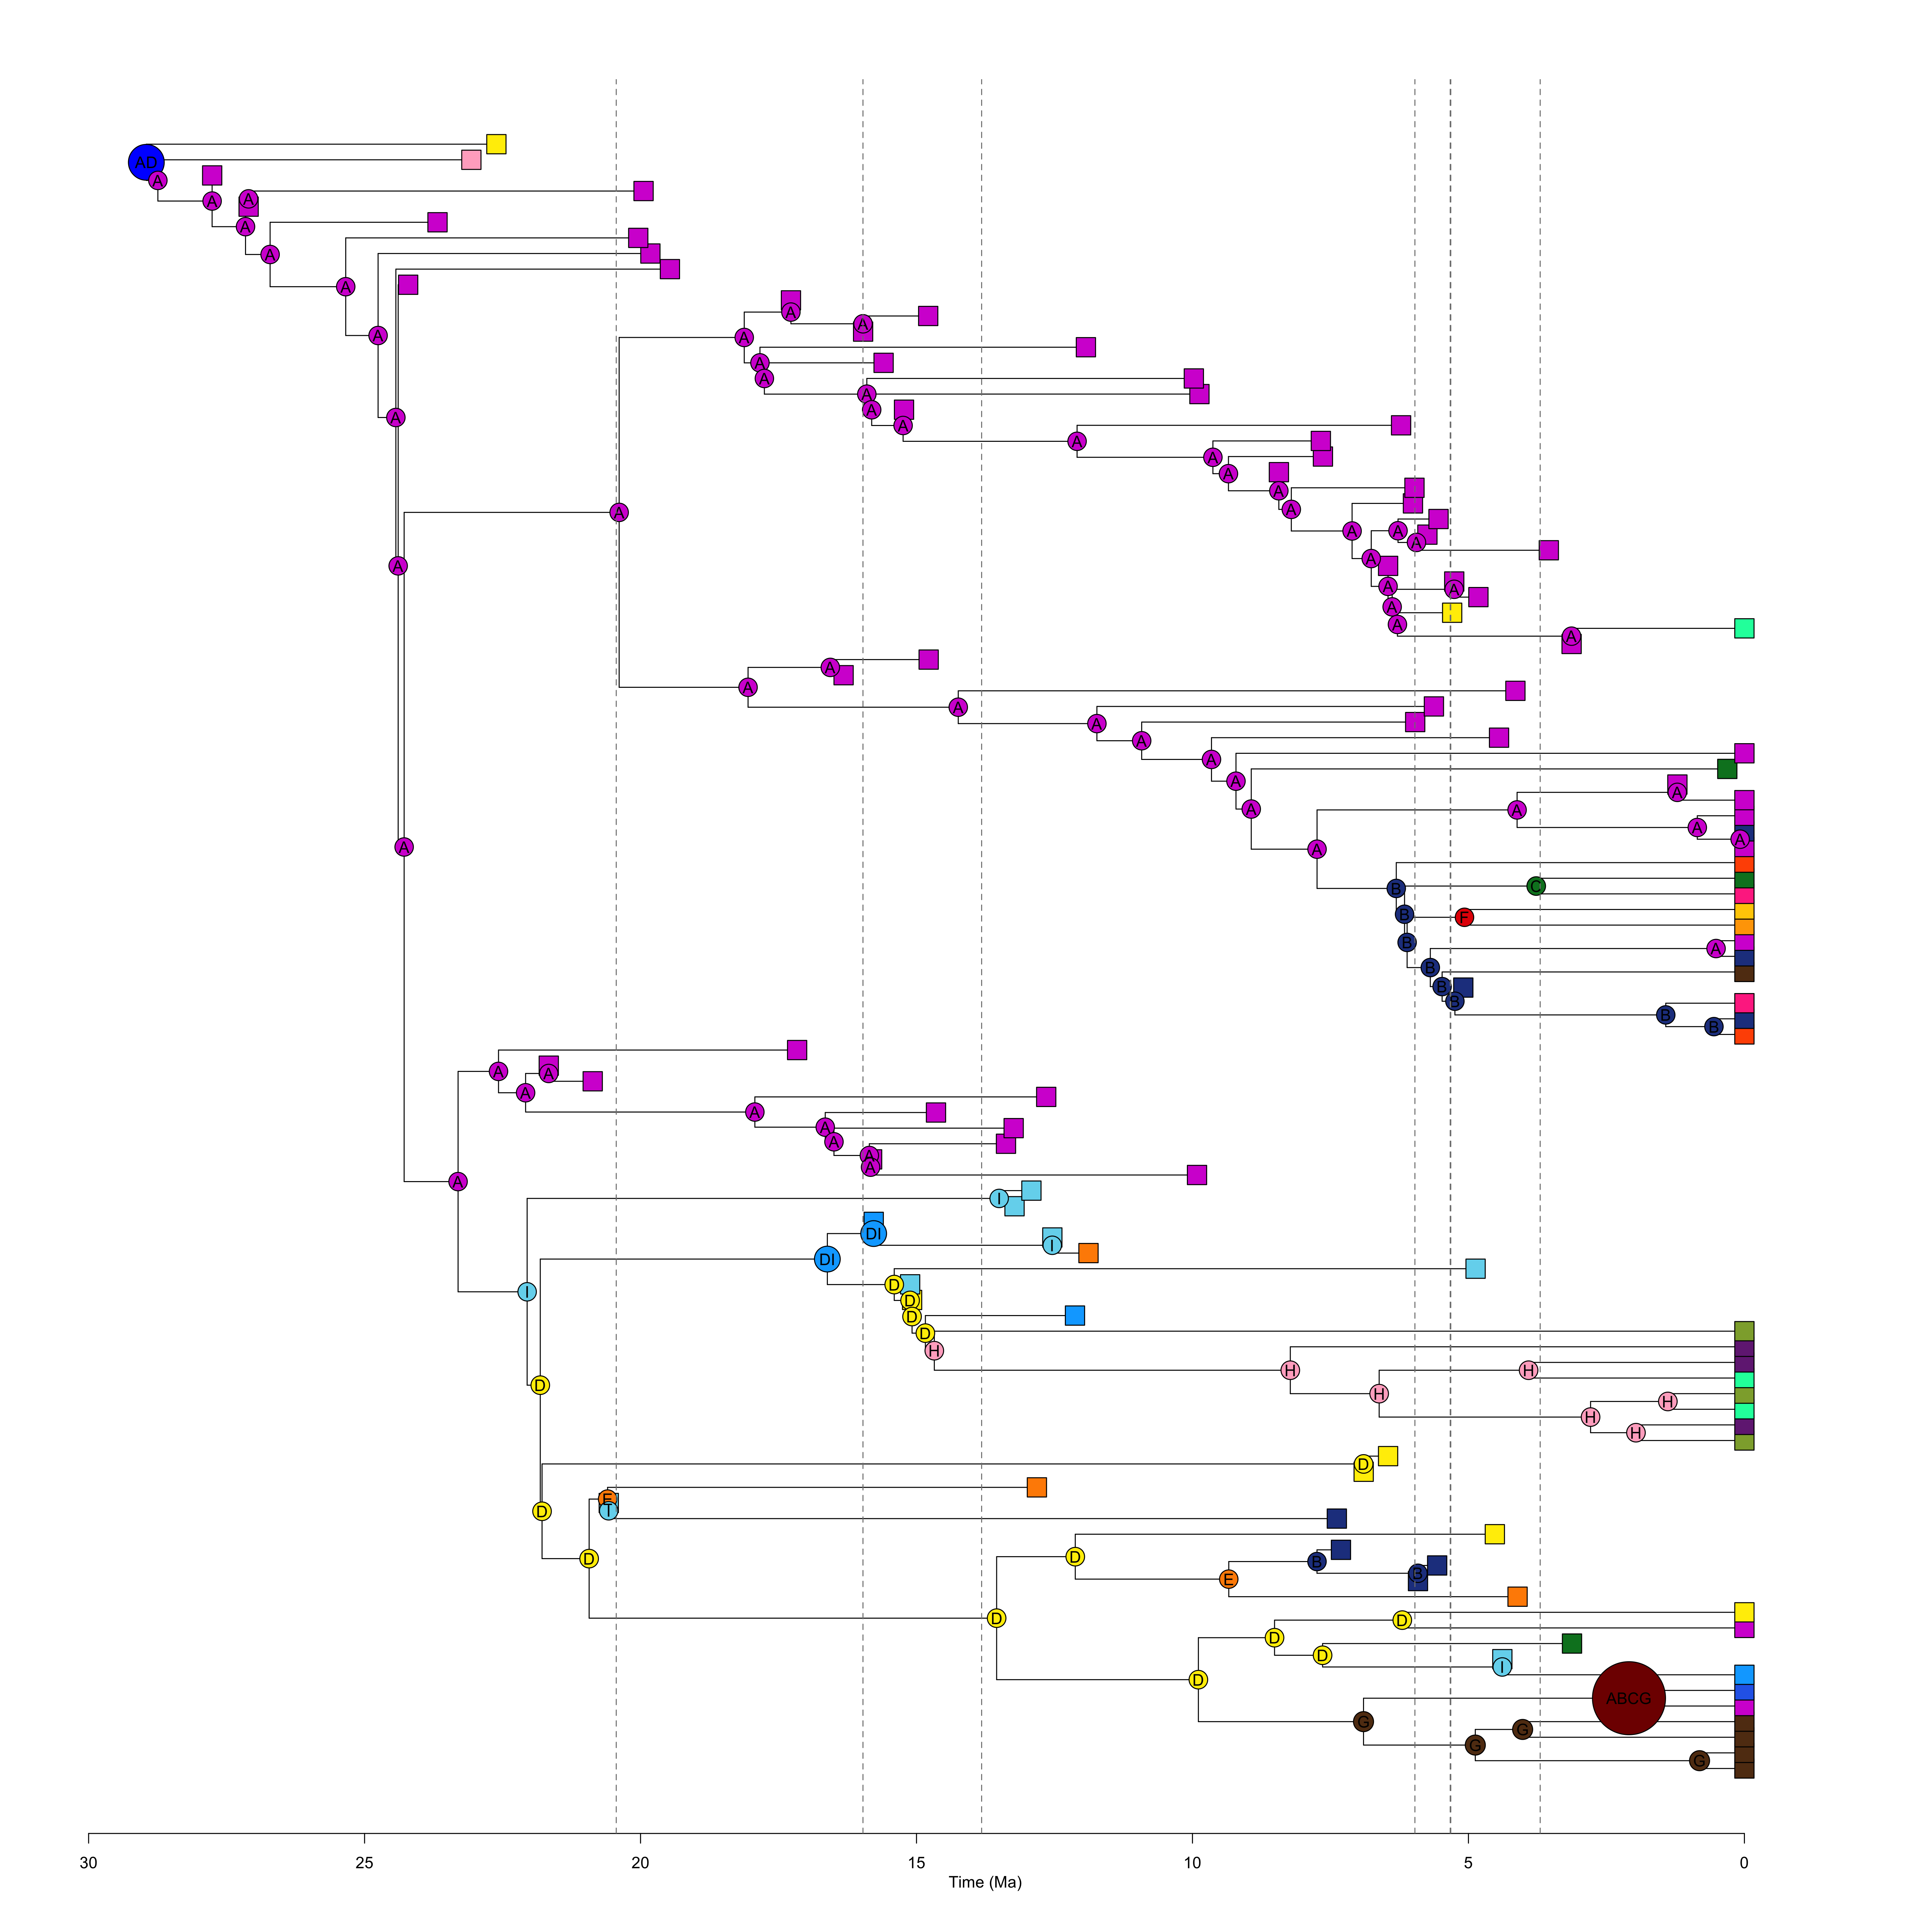
\includegraphics[width = \linewidth]{figures/all-pinnipeds-DECj-unlikely-MLstates.png}
%  \caption{All pinnipeds, DEC+J model, impossible and unlikely states removed. Nodes show Maximum Likelihood states.}
%  \label{fig-all-decj-ml-unlikely}
%\end{figure} 

% figure
%\begin{figure}[H]
% \centering
%  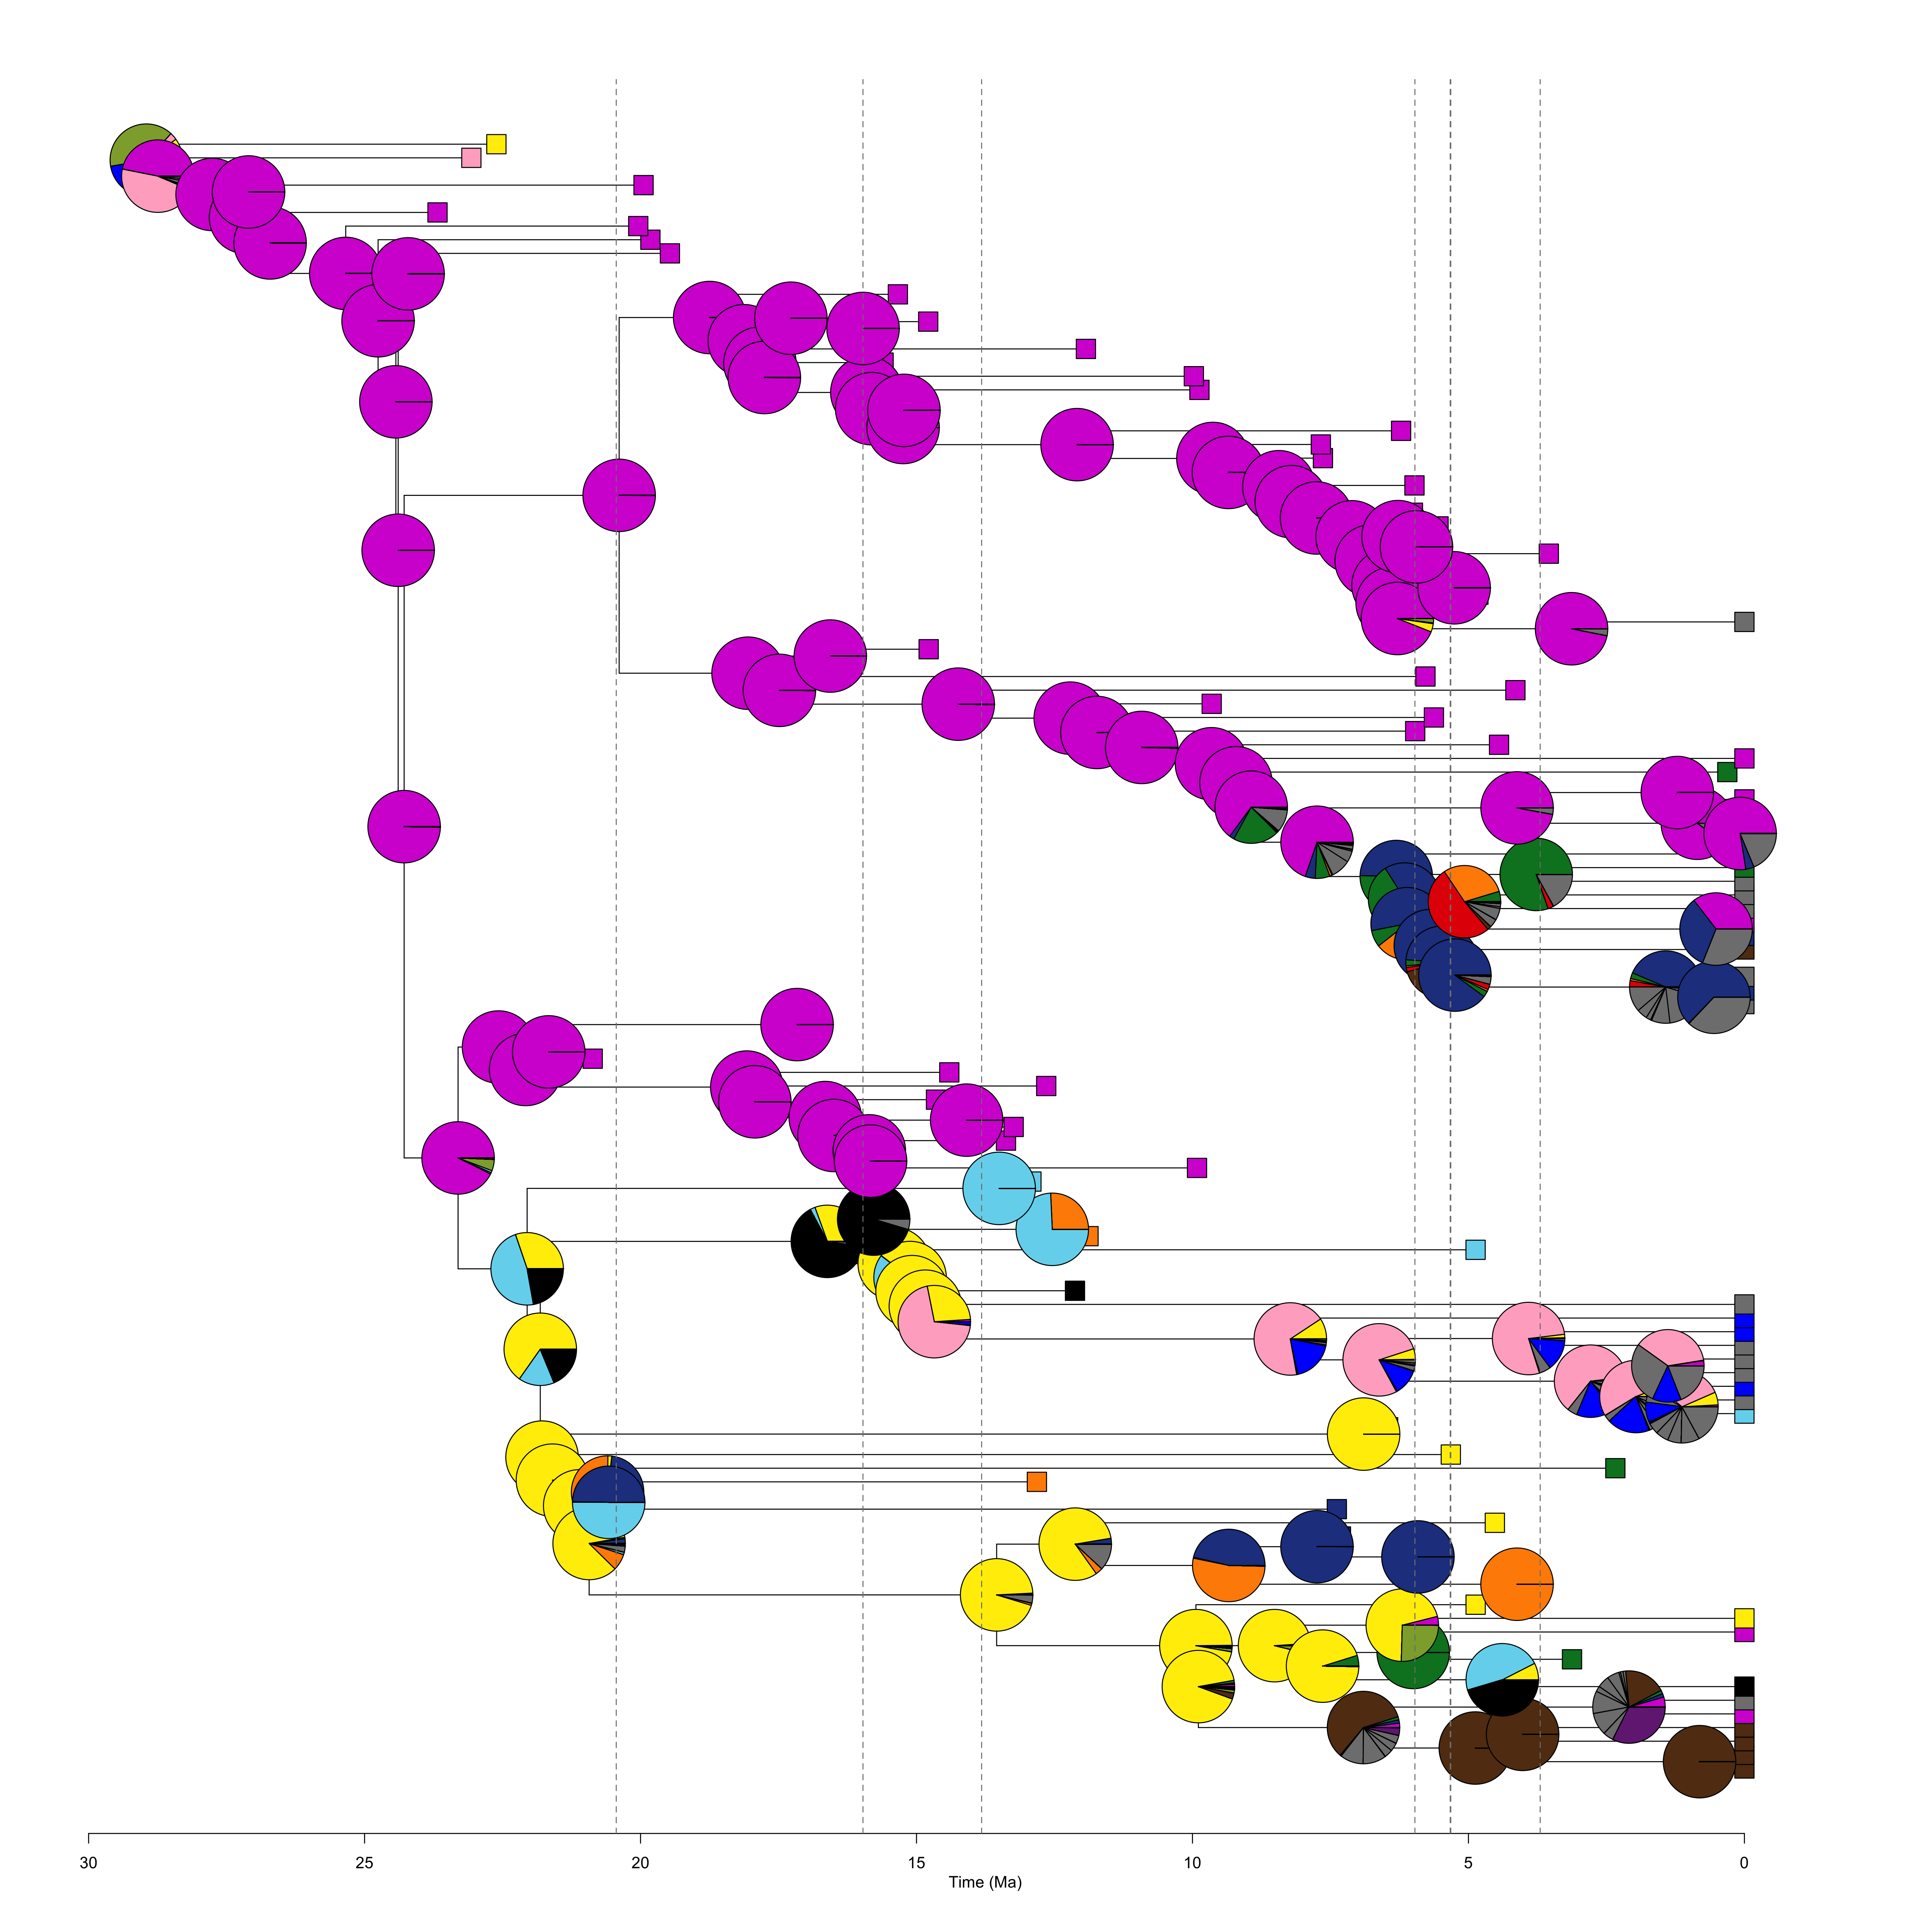
\includegraphics[width = \linewidth]{figures/all-pinnipeds-DECj-unlikely-pies.png}
%  \caption{All pinnipeds, DEC+J model, impossible and unlikely states removed. Nodes show relative probabilities of each state.}
%  \label{fig-all-decj-pie-unlikely}
%\end{figure} 

%-----------------------------------------------------------------------------------
\subsubsection{Fossil pinnipeds only}

% figure
%\begin{figure}[H]
% \centering
%  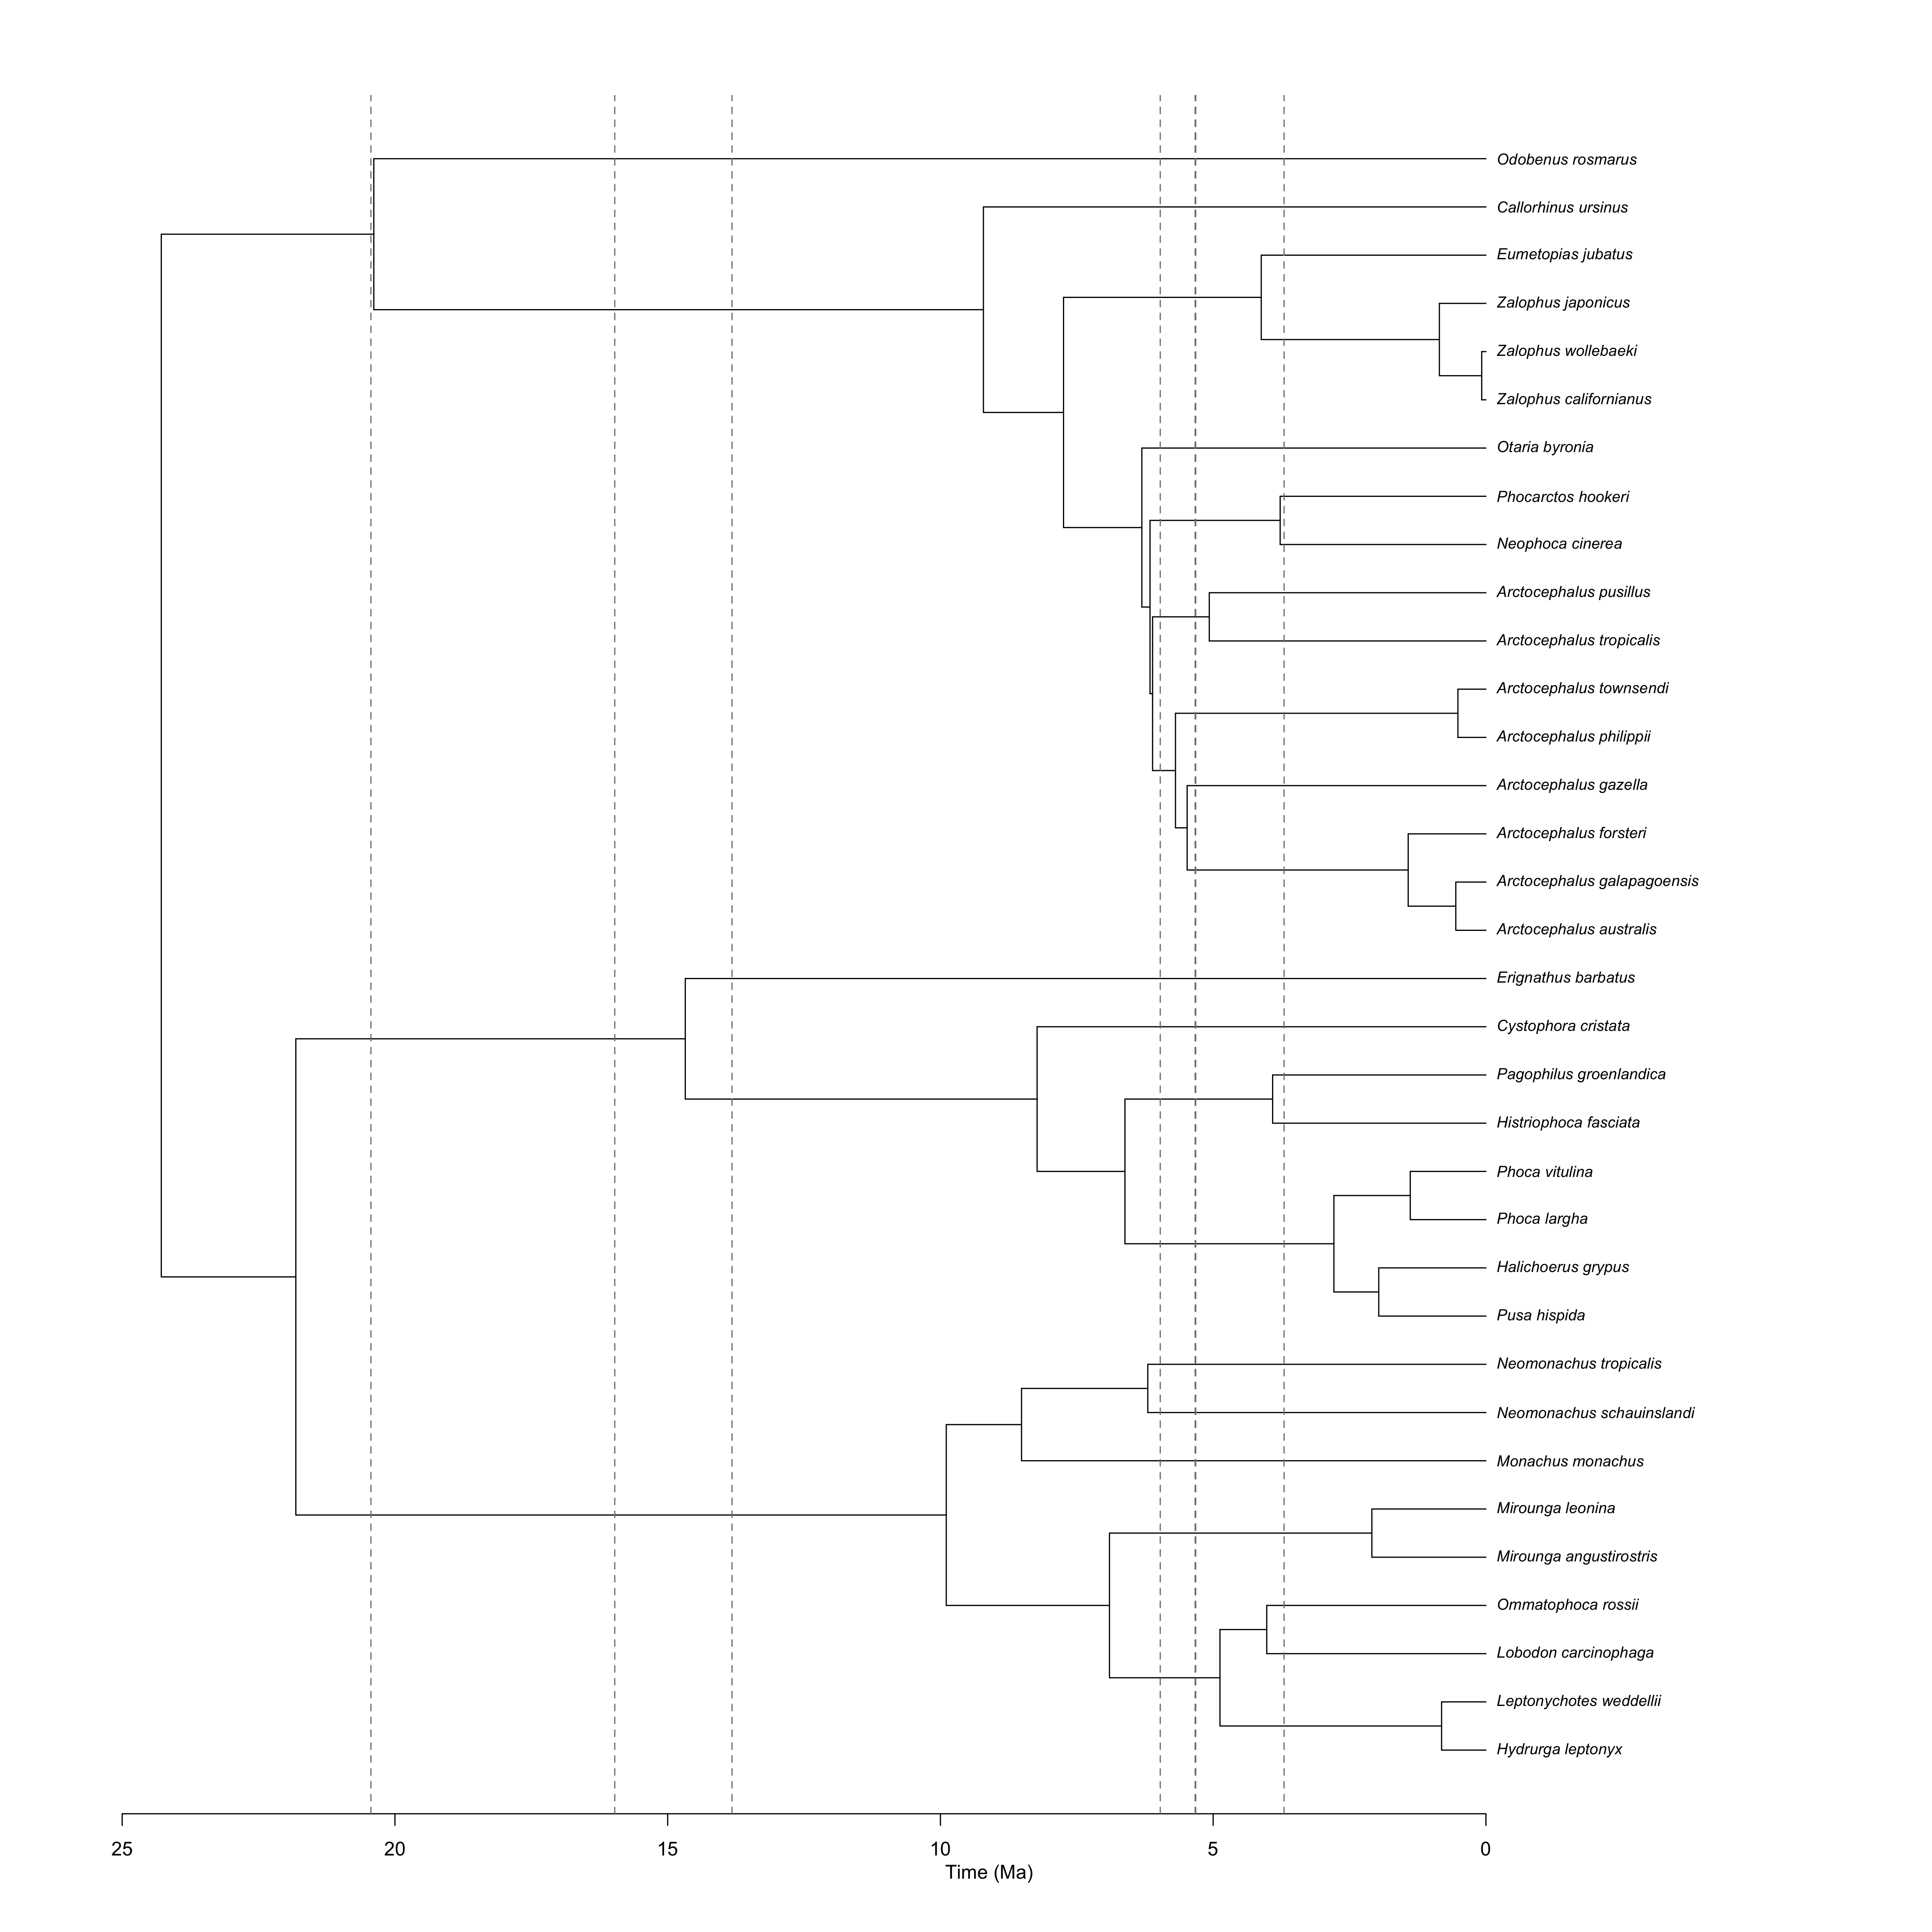
\includegraphics[width = \linewidth]{figures/fossil-pinnipeds-tree.png}
%  \caption{Phylogeny of fossil pinnipeds with taxon names to aid understanding of the following results which have taxon names removed to improve readability.}
%  \label{fig-fossil-tree}
%\end{figure} 

% figure
%\begin{figure}[H]
% \centering
%  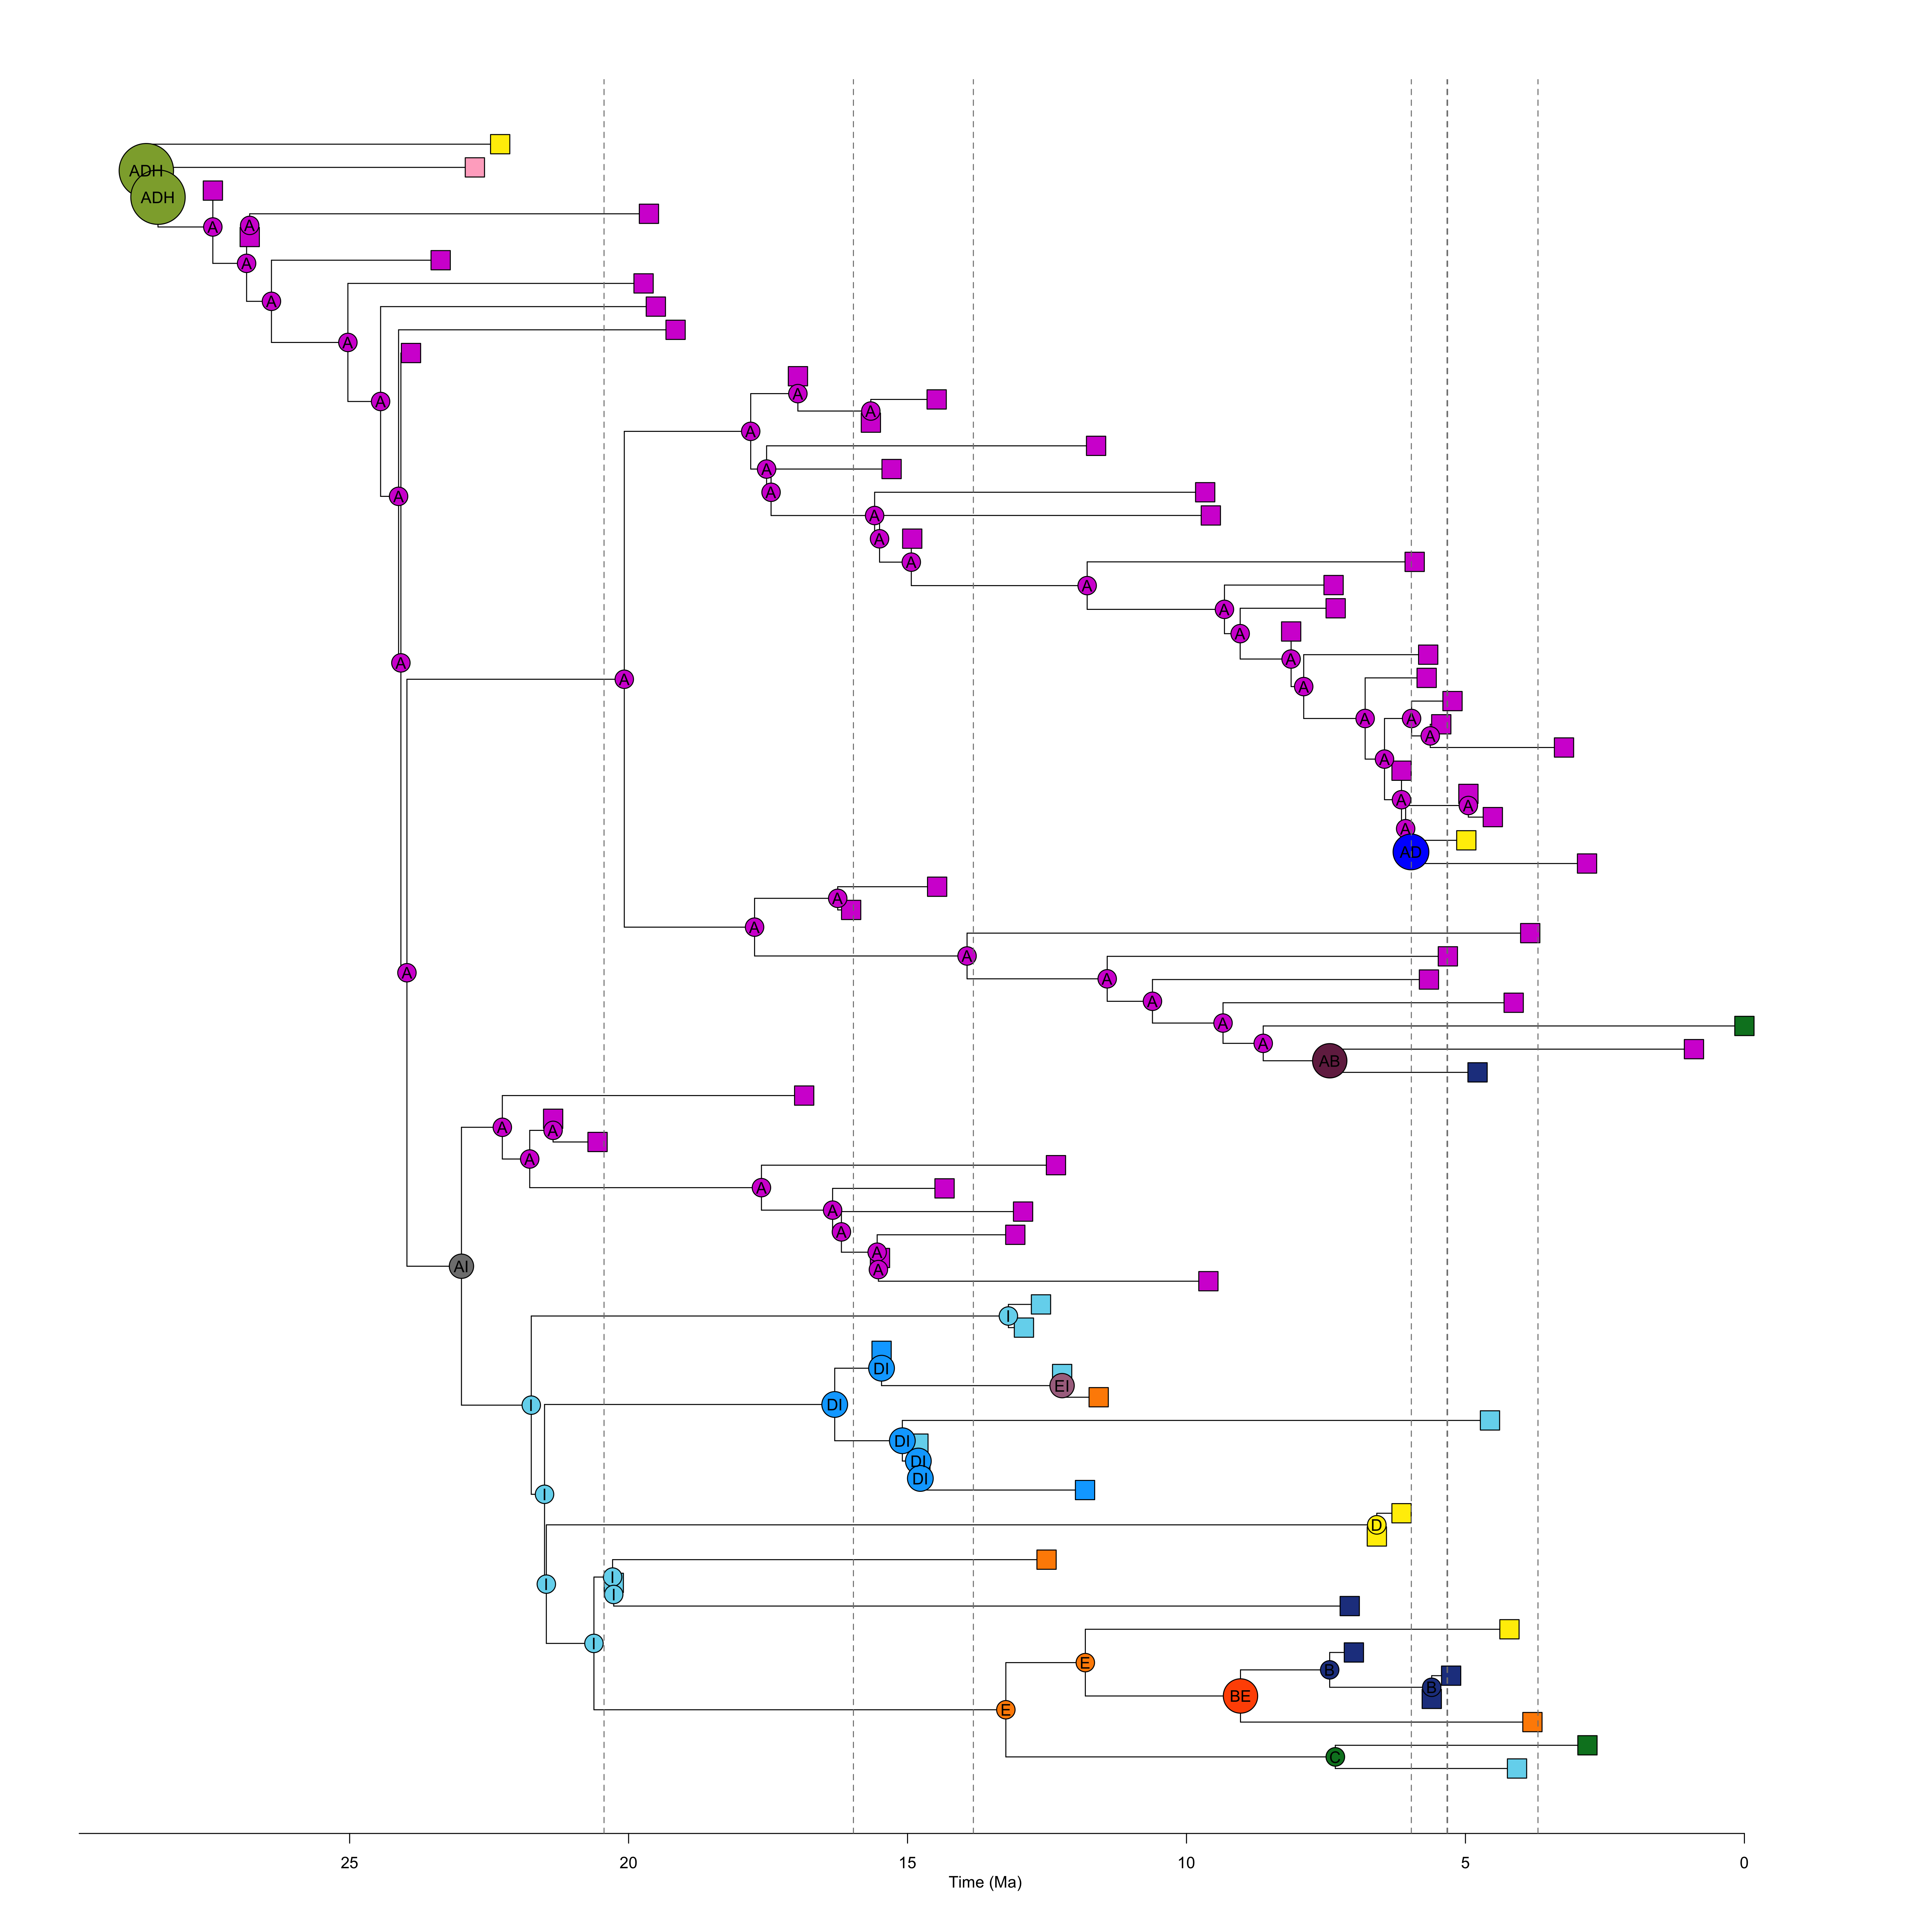
\includegraphics[width = \linewidth]{figures/fossil-pinnipeds-DEC-impossible-MLstates.png}
%  \caption{Fossil pinnipeds only, DEC model, impossible states removed. Nodes show Maximum Likelihood states.}
%  \label{fig-fossil-dec-ml}
%\end{figure} 

% figure
%\begin{figure}[H]
% \centering
%  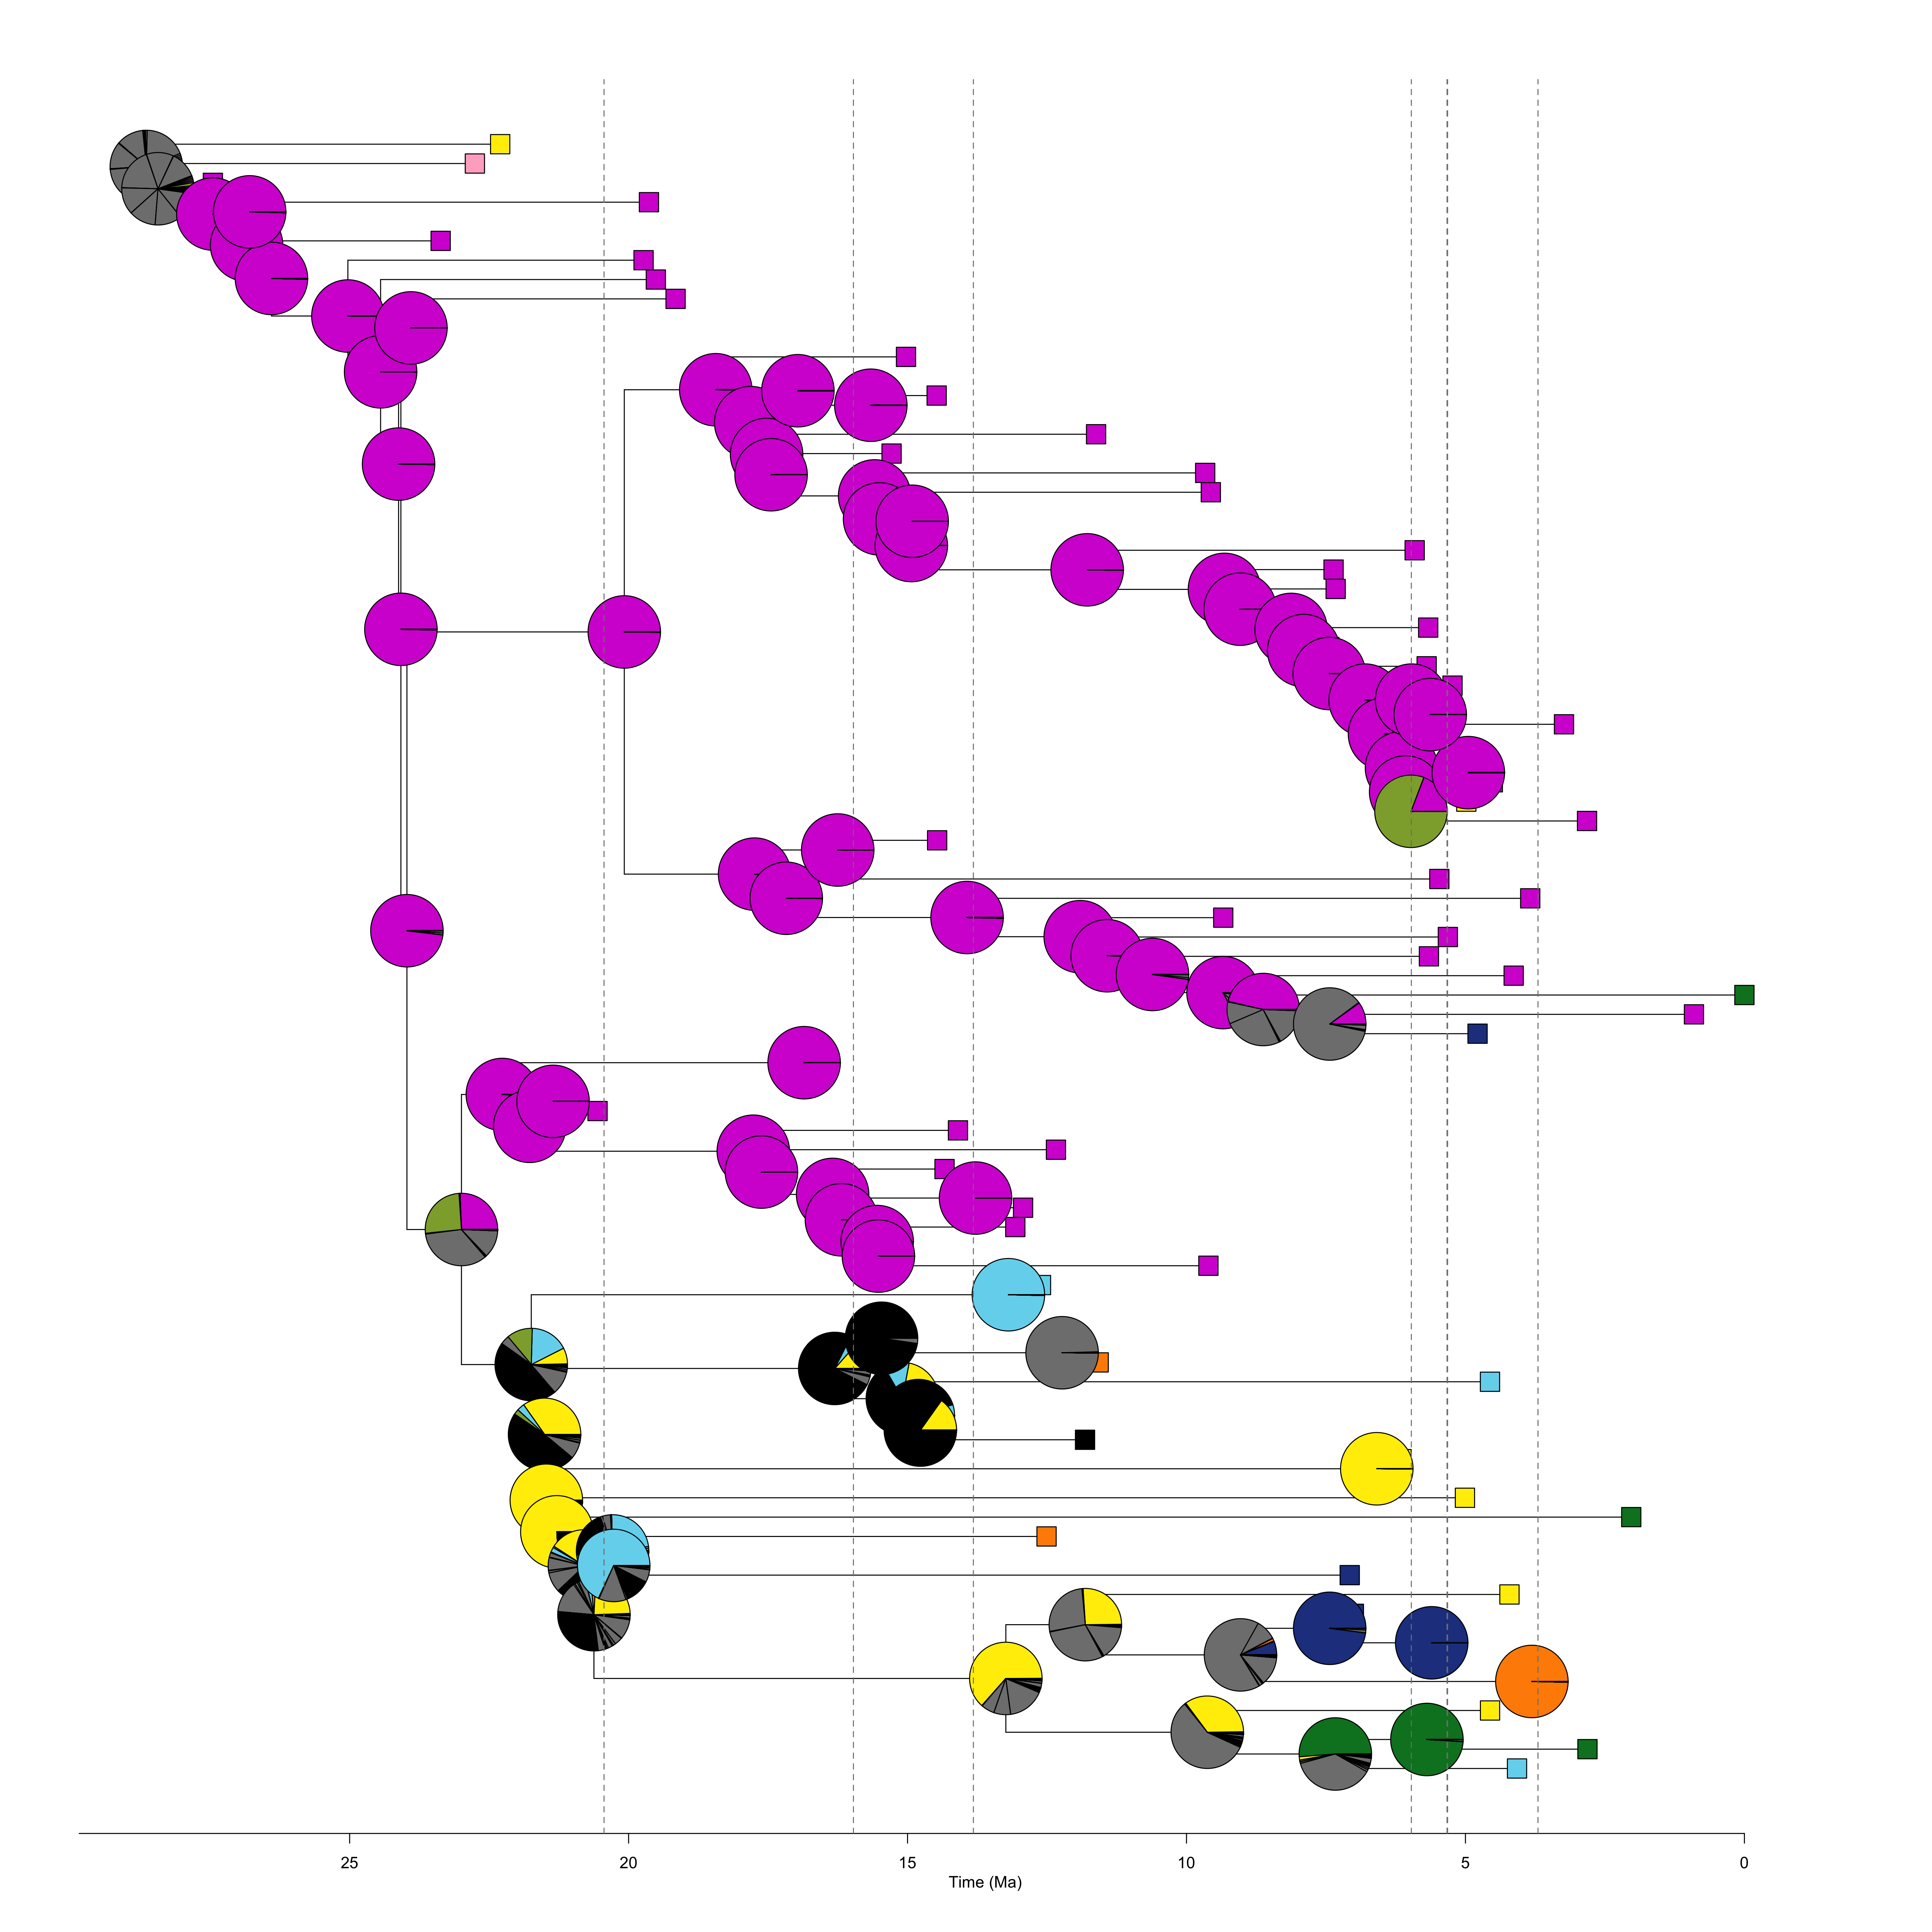
\includegraphics[width = \linewidth]{figures/fossil-pinnipeds-DEC-impossible-pies.png}
%  \caption{Fossil pinnipeds only, DEC model, impossible states removed. Nodes show relative probabilities of each state.}
%  \label{fig-fossil-dec-pie}
%\end{figure} 

% figure
%\begin{figure}[H]
% \centering
%  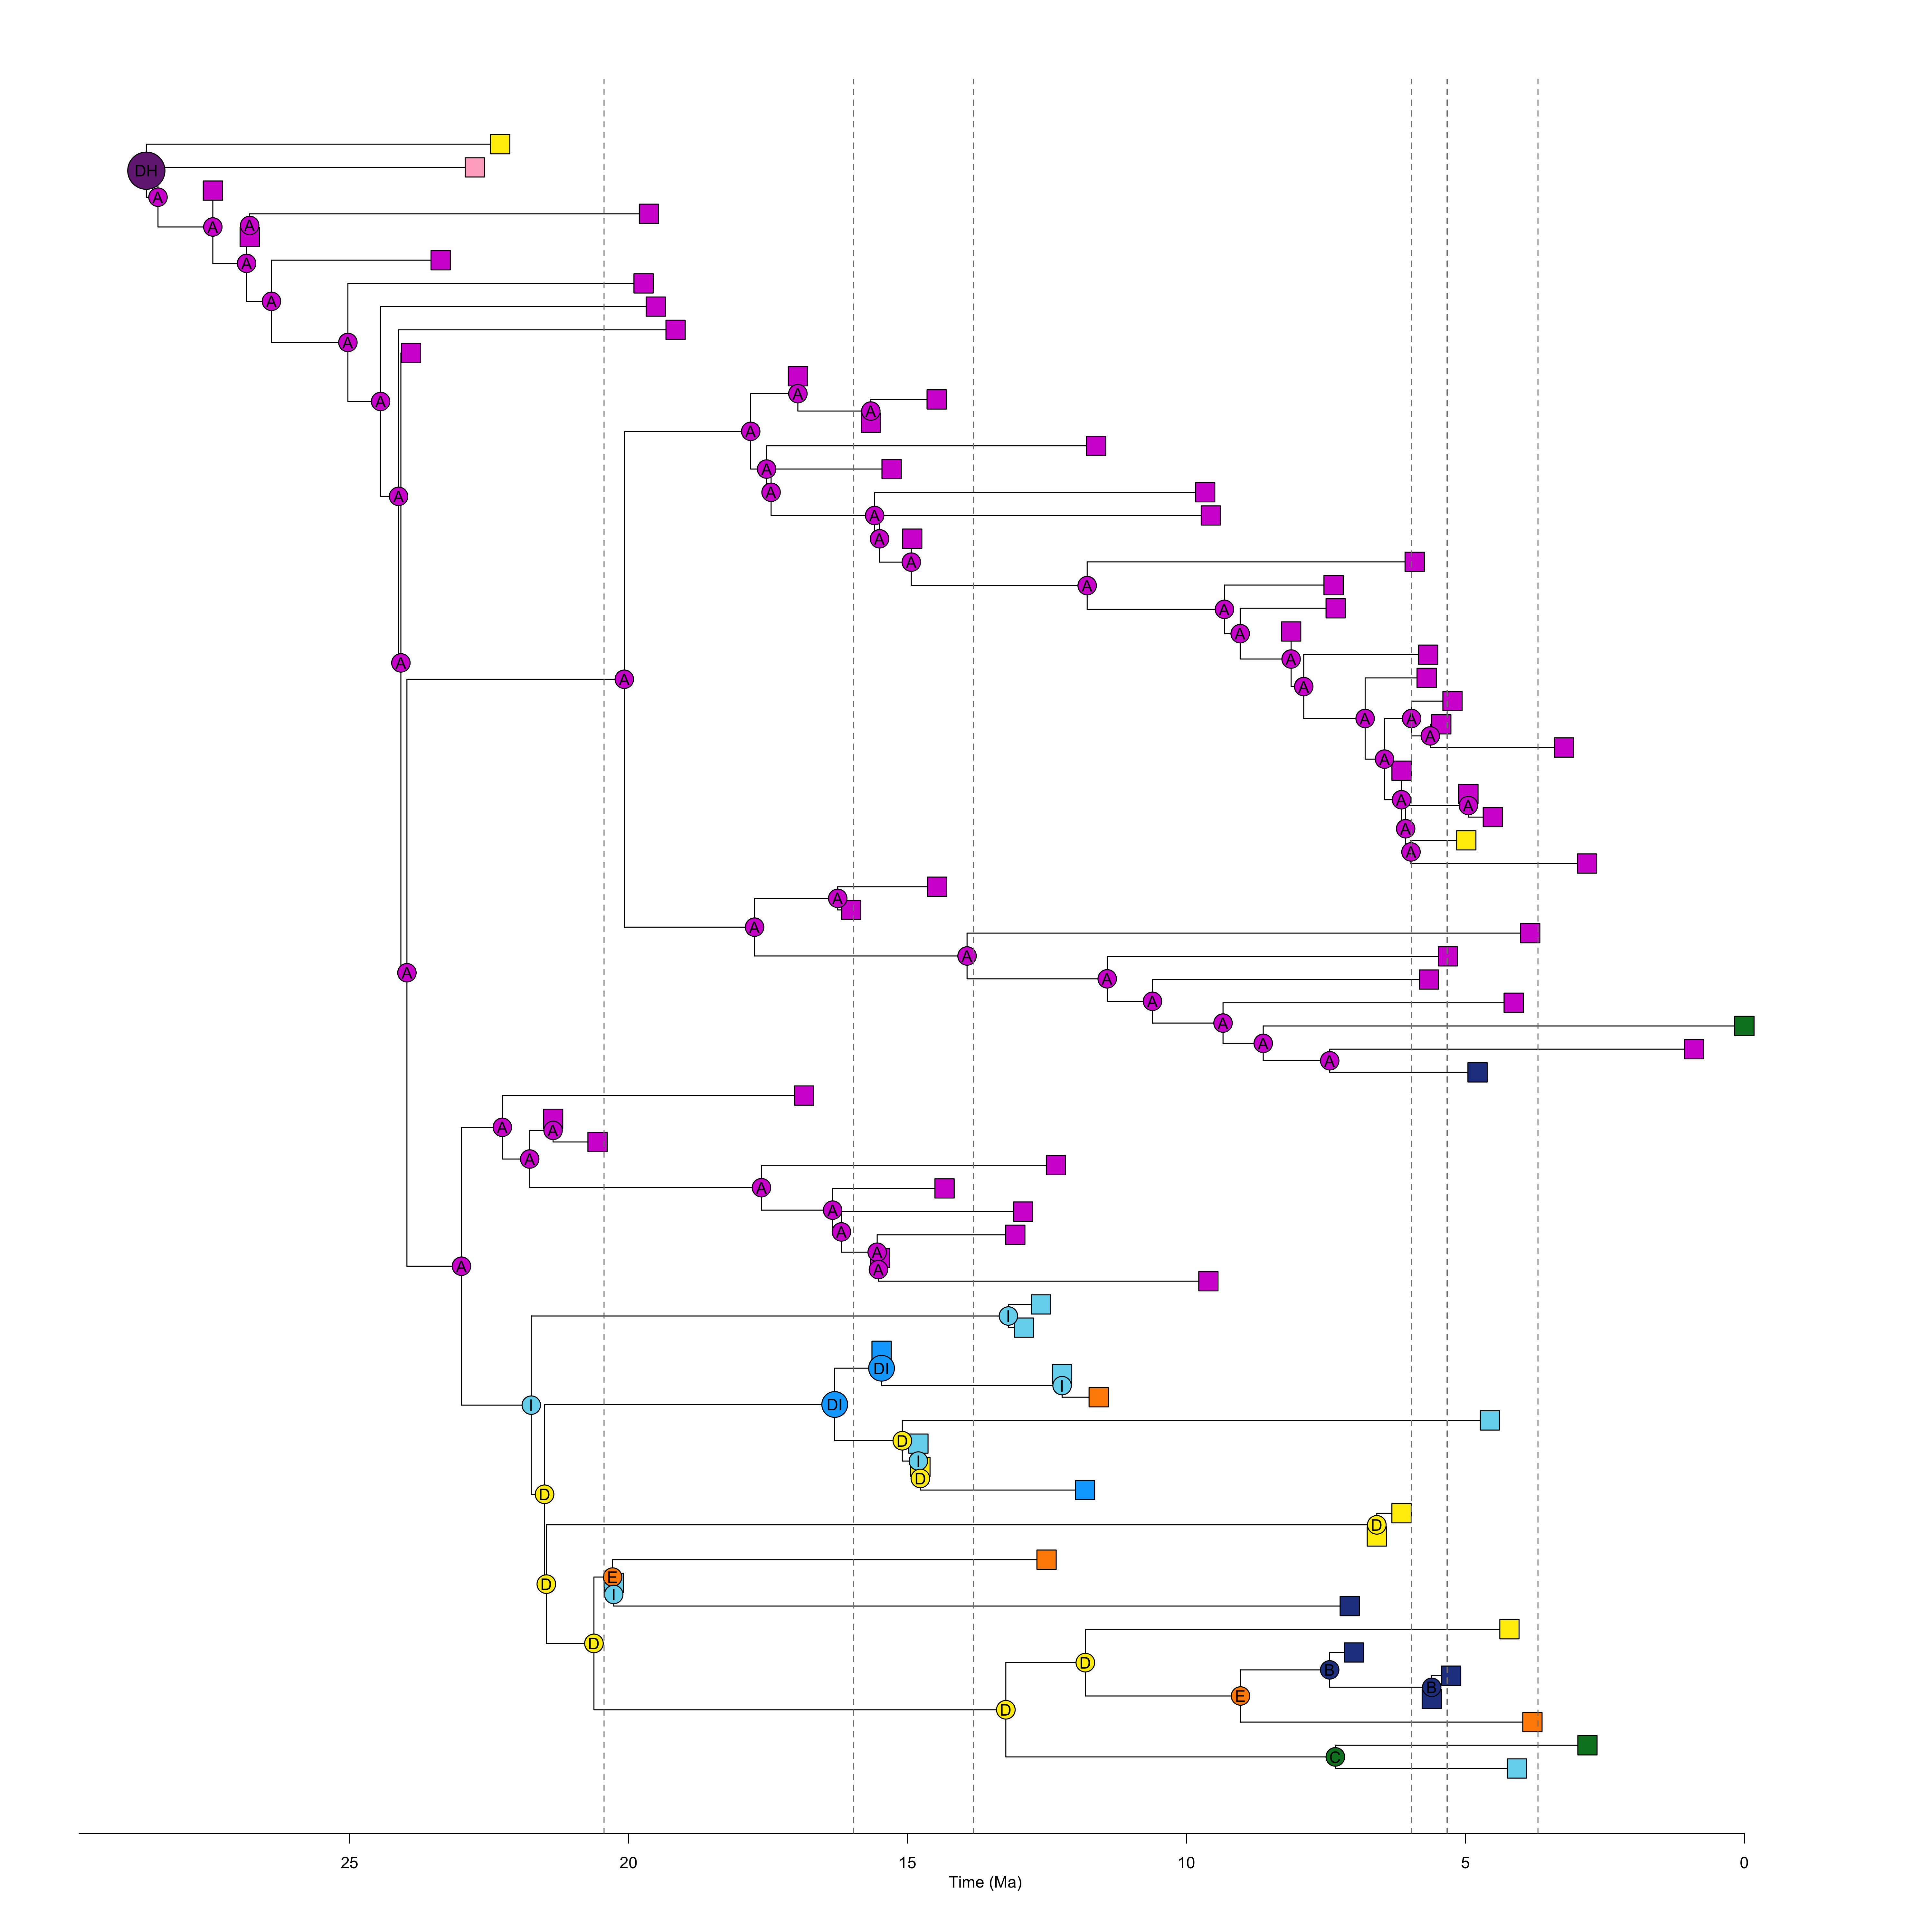
\includegraphics[width = \linewidth]{figures/fossil-pinnipeds-DECj-impossible-MLstates.png}
%  \caption{Fossil pinnipeds only, DEC+J model, impossible states removed. Nodes show Maximum Likelihood states.}
%  \label{fig-fossil-decj-ml}
%\end{figure} 

% figure
%\begin{figure}[H]
% \centering
%  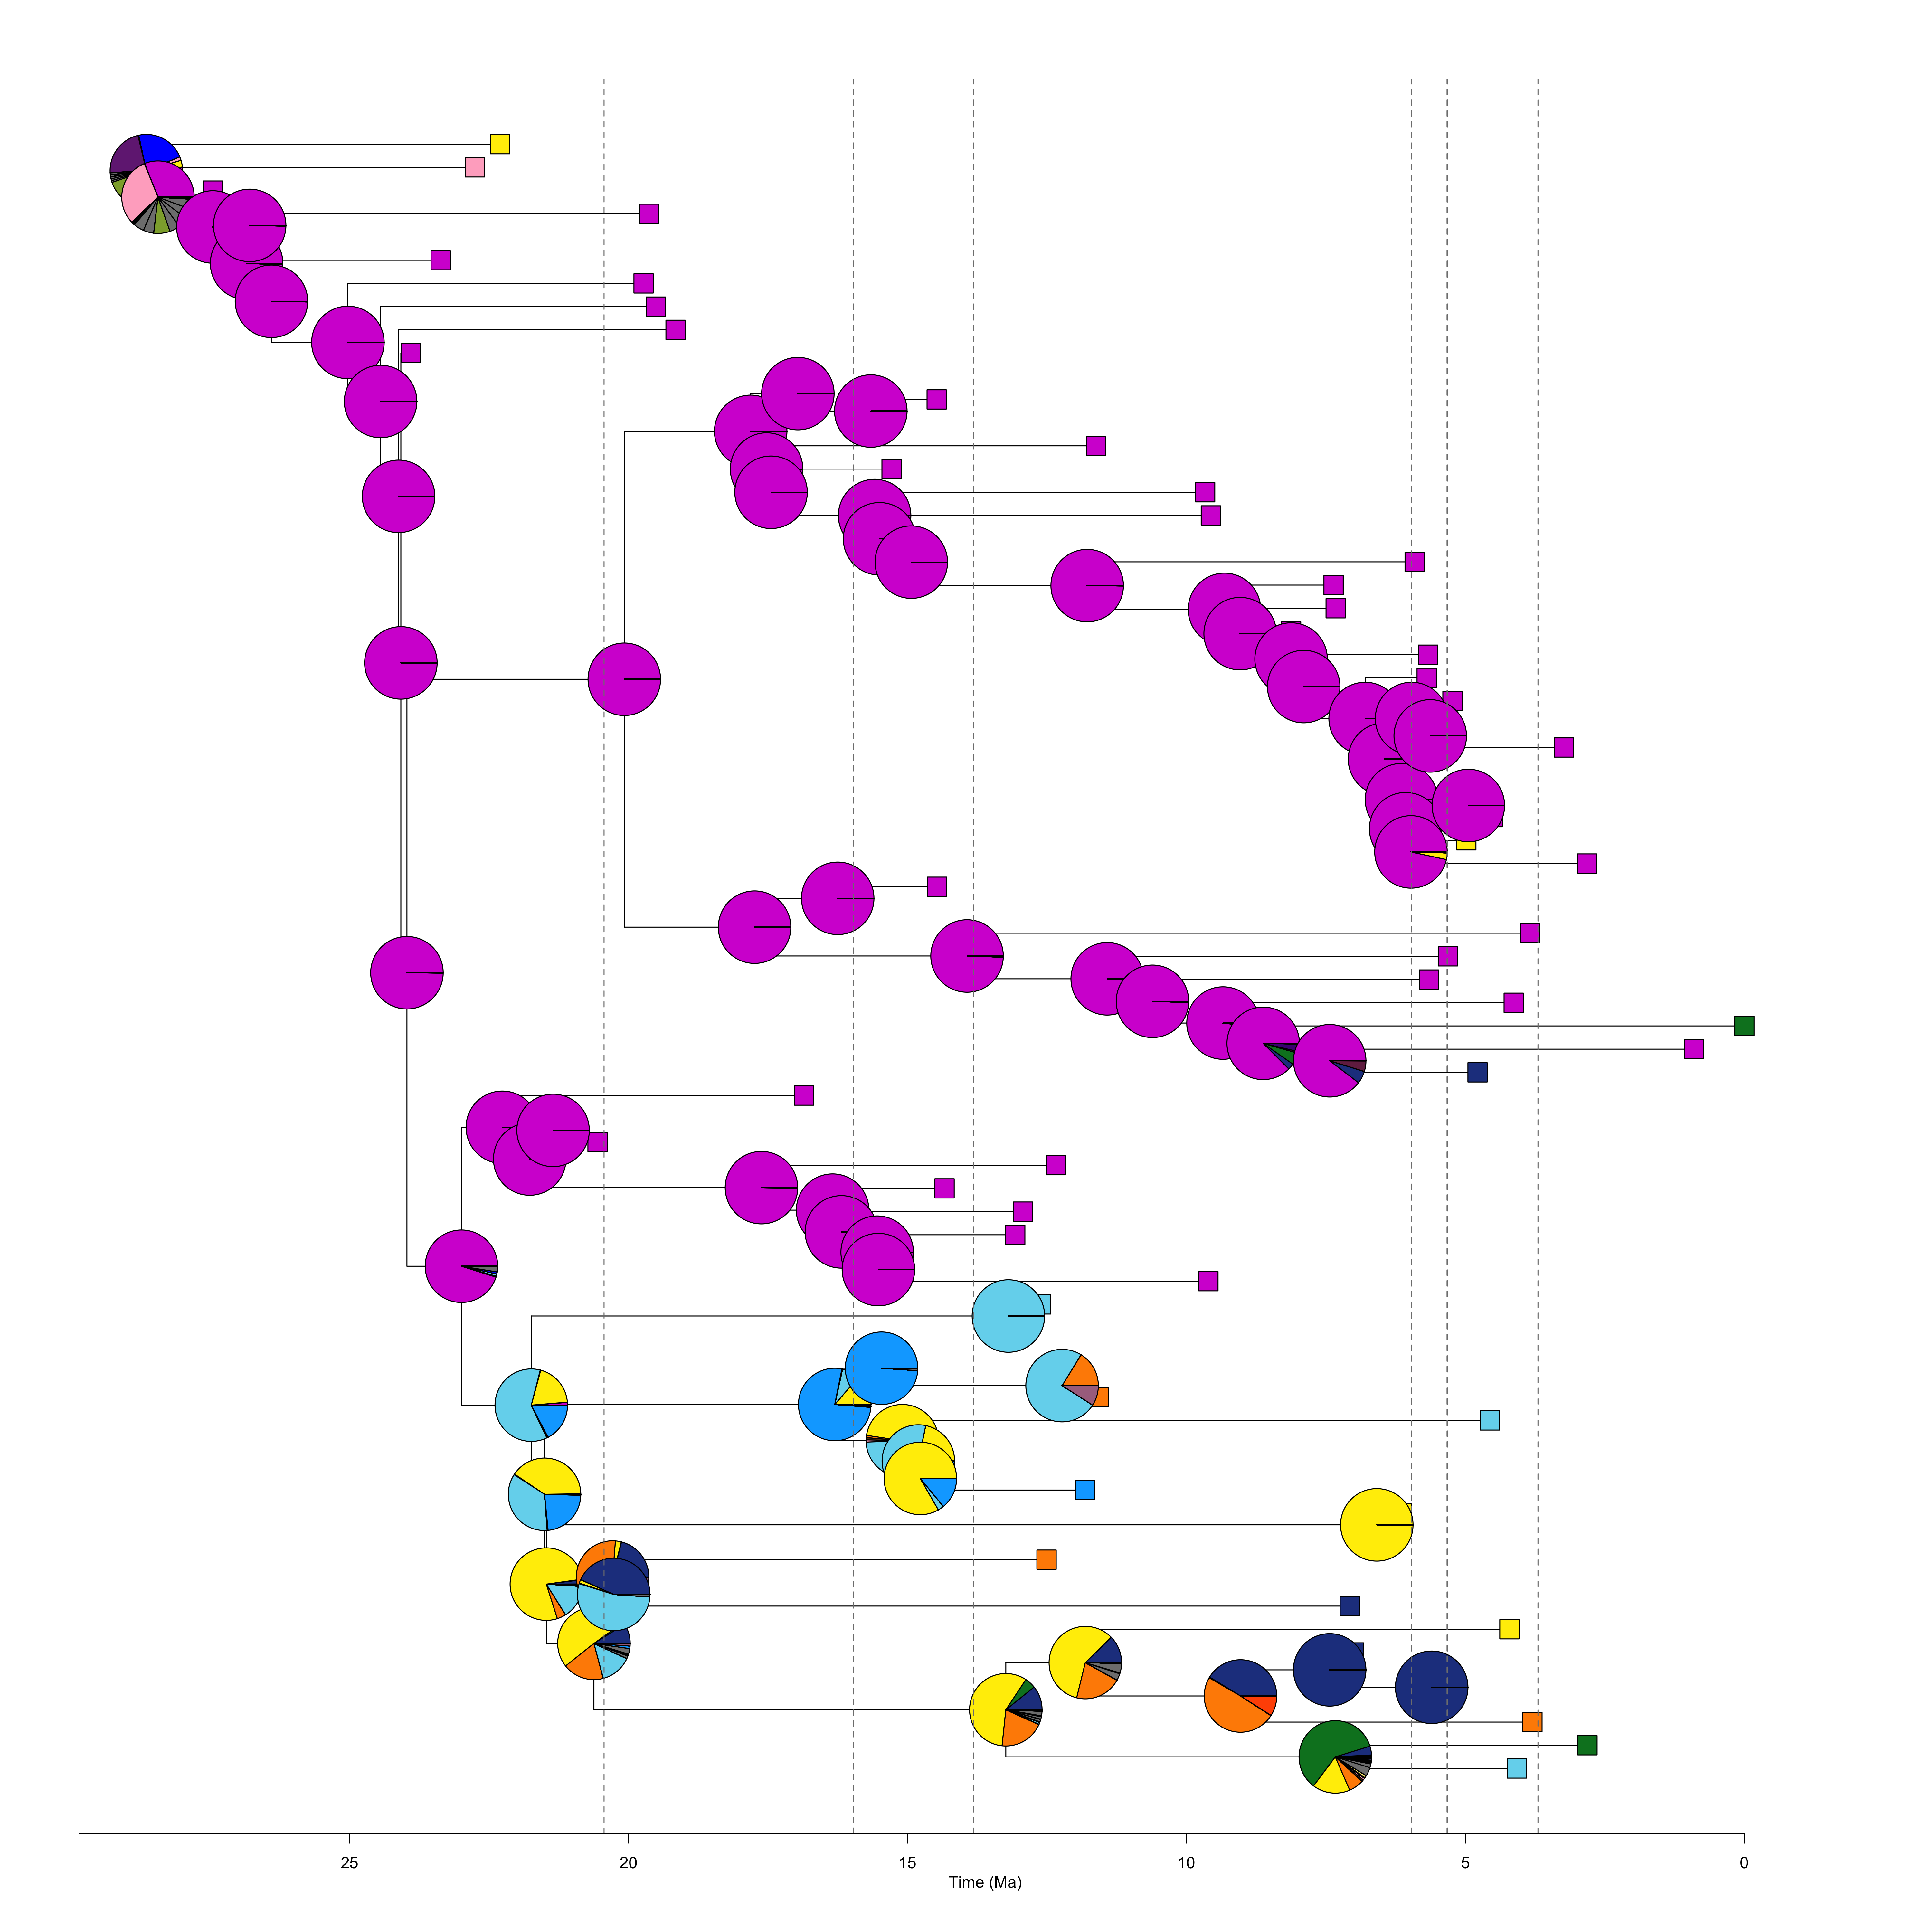
\includegraphics[width = \linewidth]{figures/fossil-pinnipeds-DECj-impossible-pies.png}
%  \caption{Fossil pinnipeds only, DEC+J model, impossible states removed. Nodes show relative probabilities of each state.}
%  \label{fig-fossil-decj-pie}
%\end{figure} 
 
%-----------------------------------------------------------------------------------
% fossil + unlikely

% figure
%\begin{figure}[H]
% \centering
%  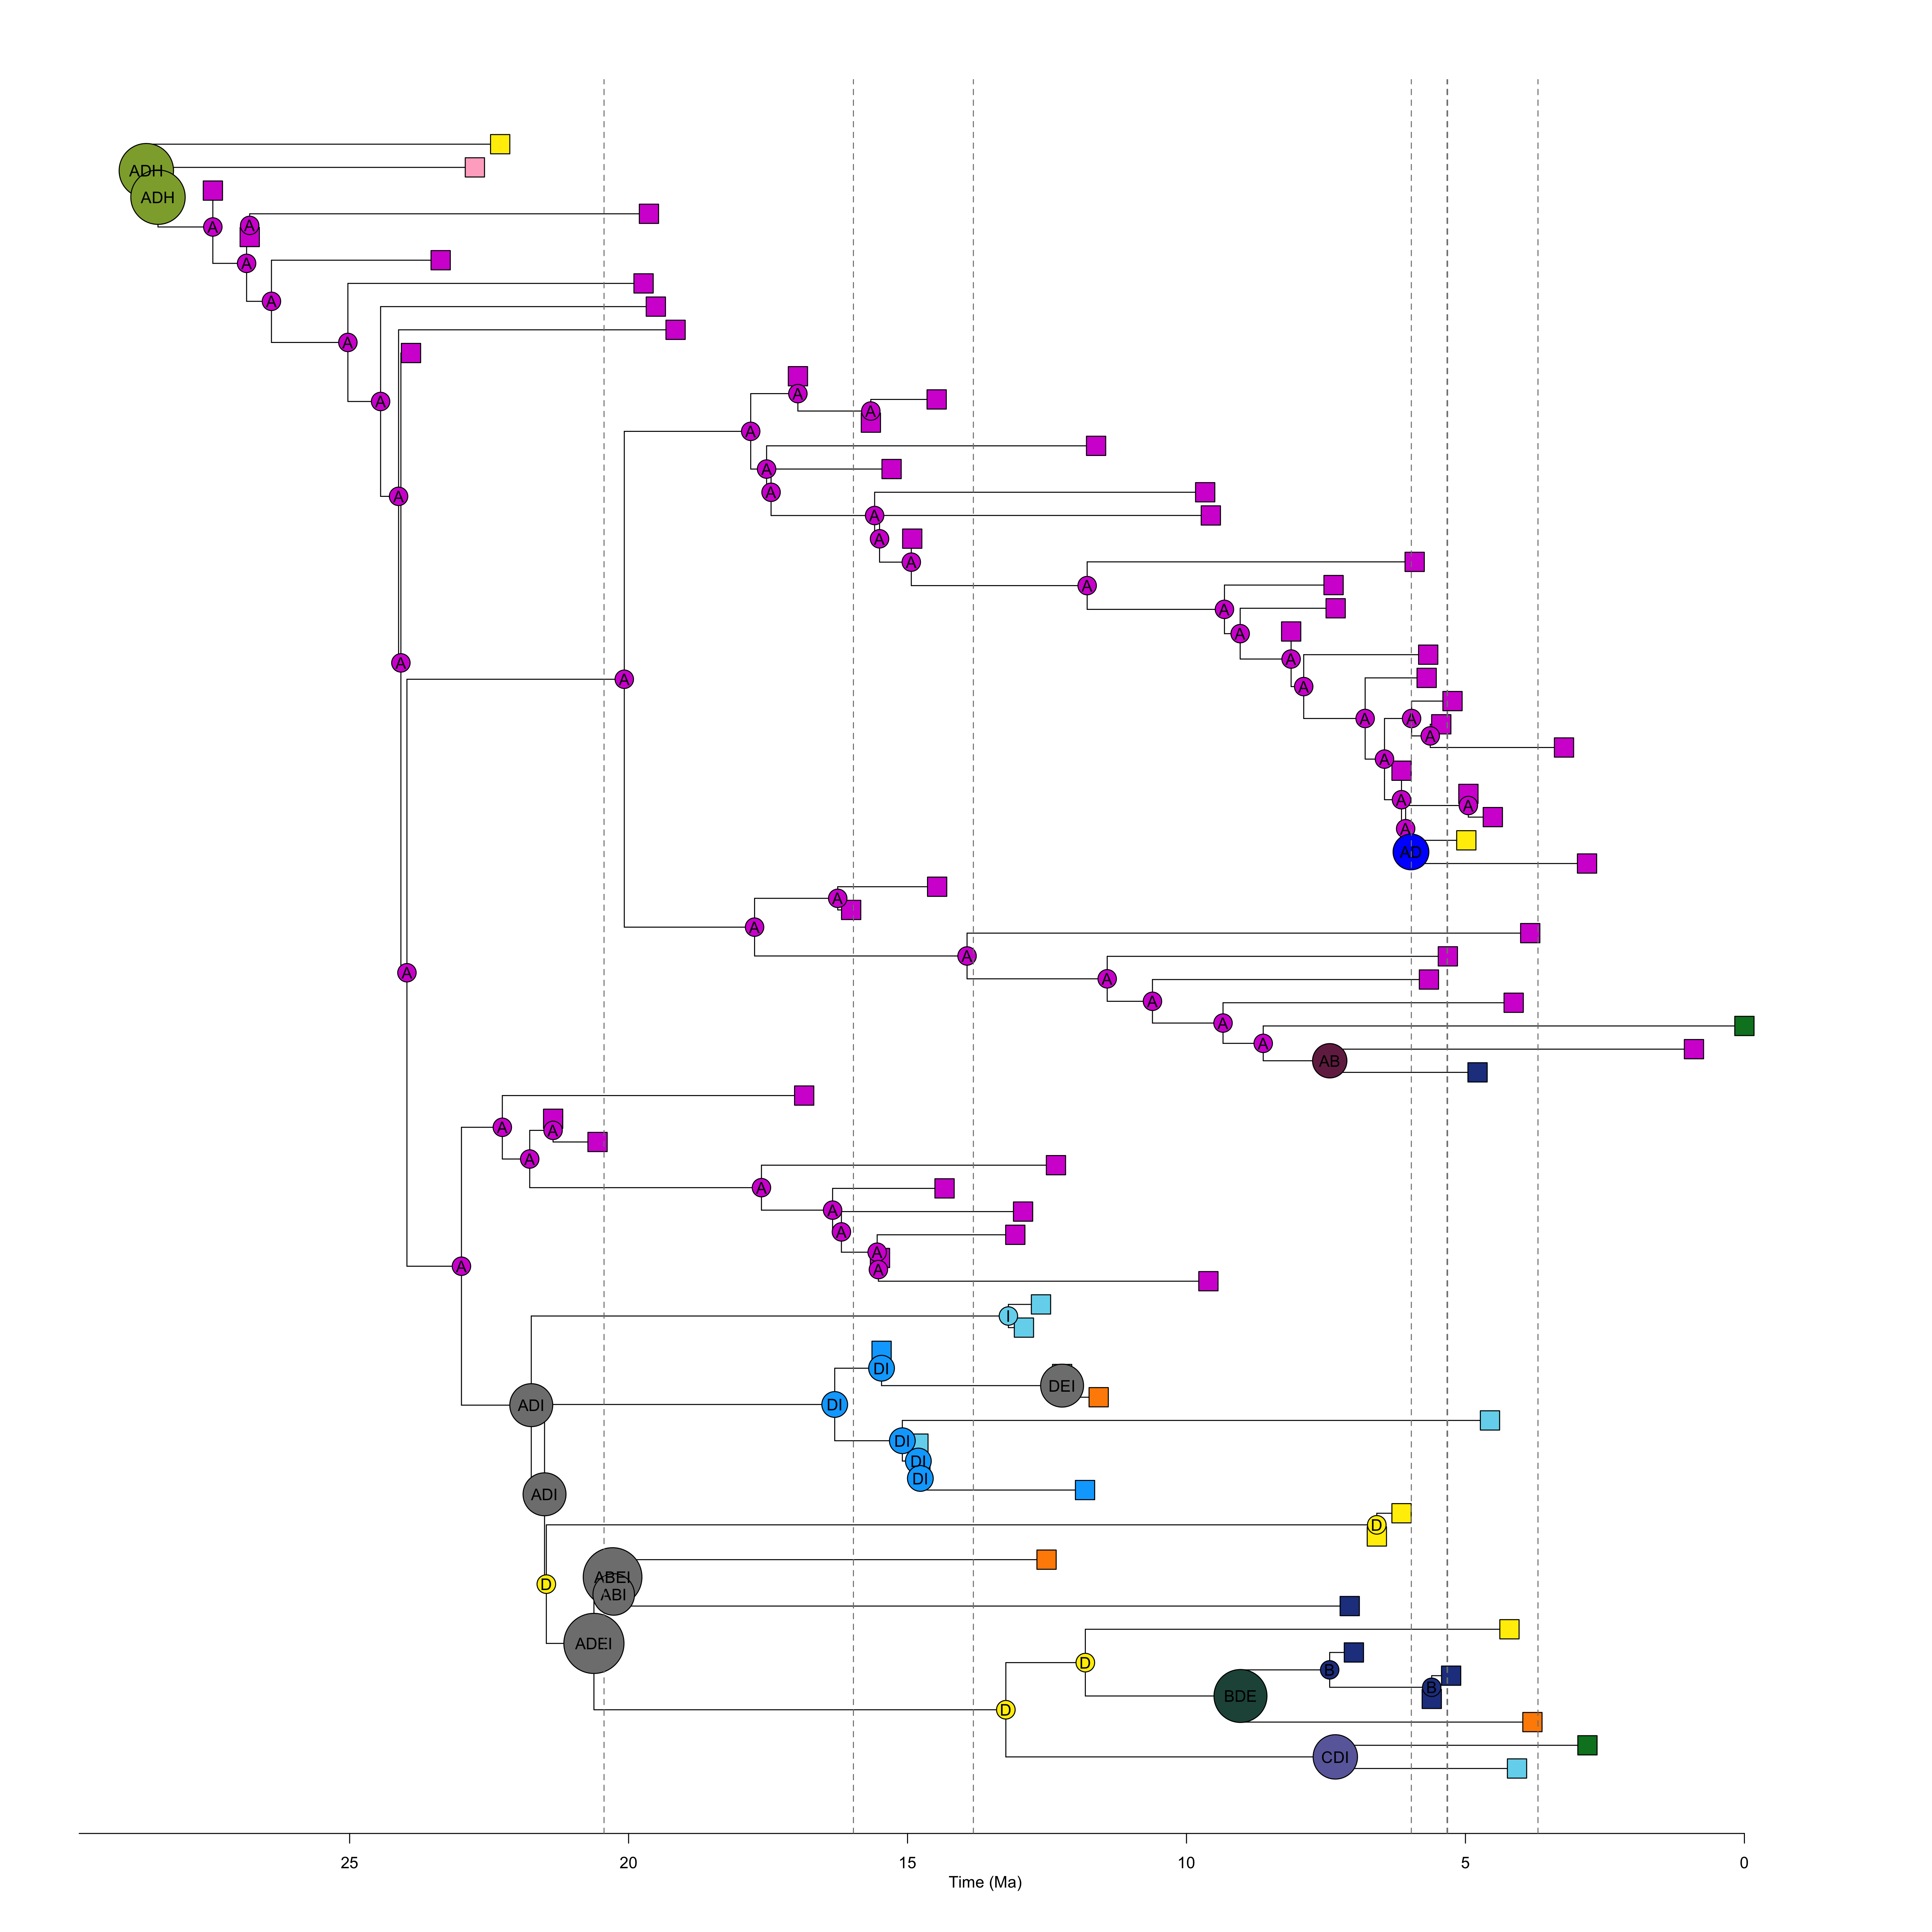
\includegraphics[width = \linewidth]{figures/fossil-pinnipeds-DEC-unlikely-MLstates.png}
%  \caption{Fossil pinnipeds only, DEC model, impossible and unlikely states removed. Nodes show Maximum Likelihood states.}
%  \label{fig-fossil-dec-ml-unlikely}
%\end{figure} 

% figure
%\begin{figure}[H]
% \centering
%  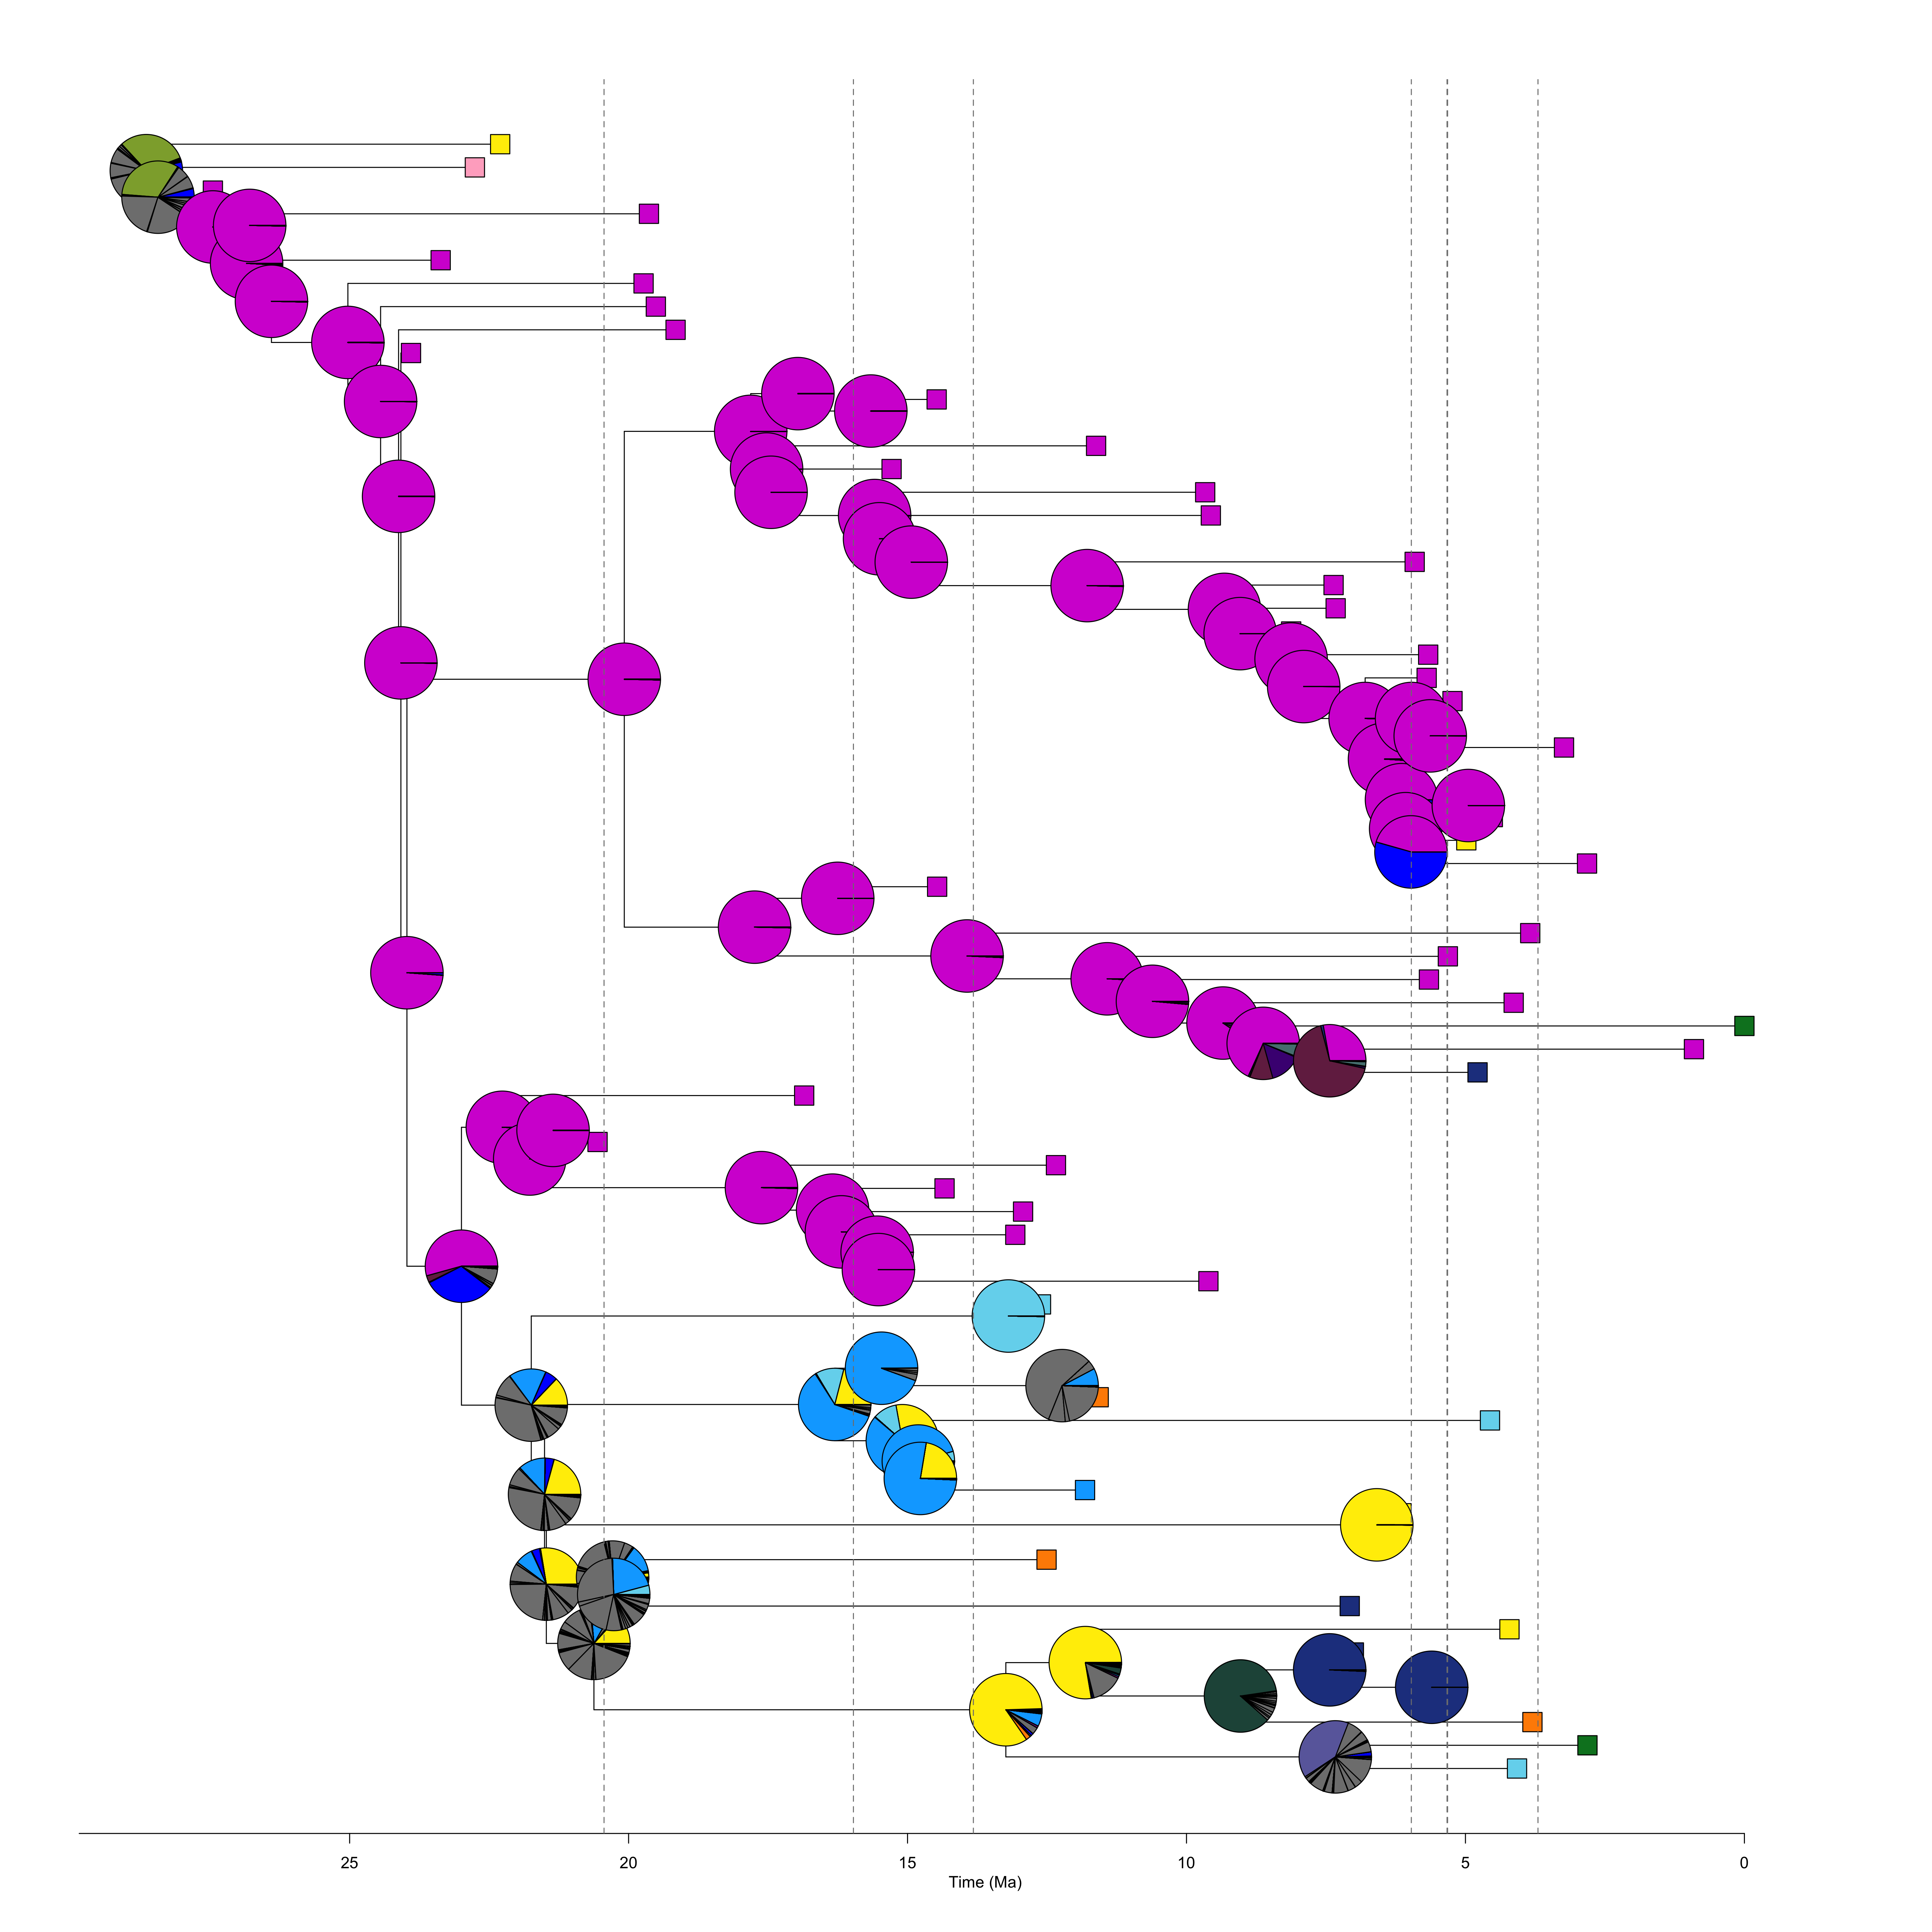
\includegraphics[width = \linewidth]{figures/fossil-pinnipeds-DEC-unlikely-pies.png}
%  \caption{Fossil pinnipeds only, DEC model, impossible and unlikely states removed. Nodes show relative probabilities of each state.}
%  \label{fig-fossil-dec-pie-unlikely}
%\end{figure} 

% figure
%\begin{figure}[H]
% \centering
%  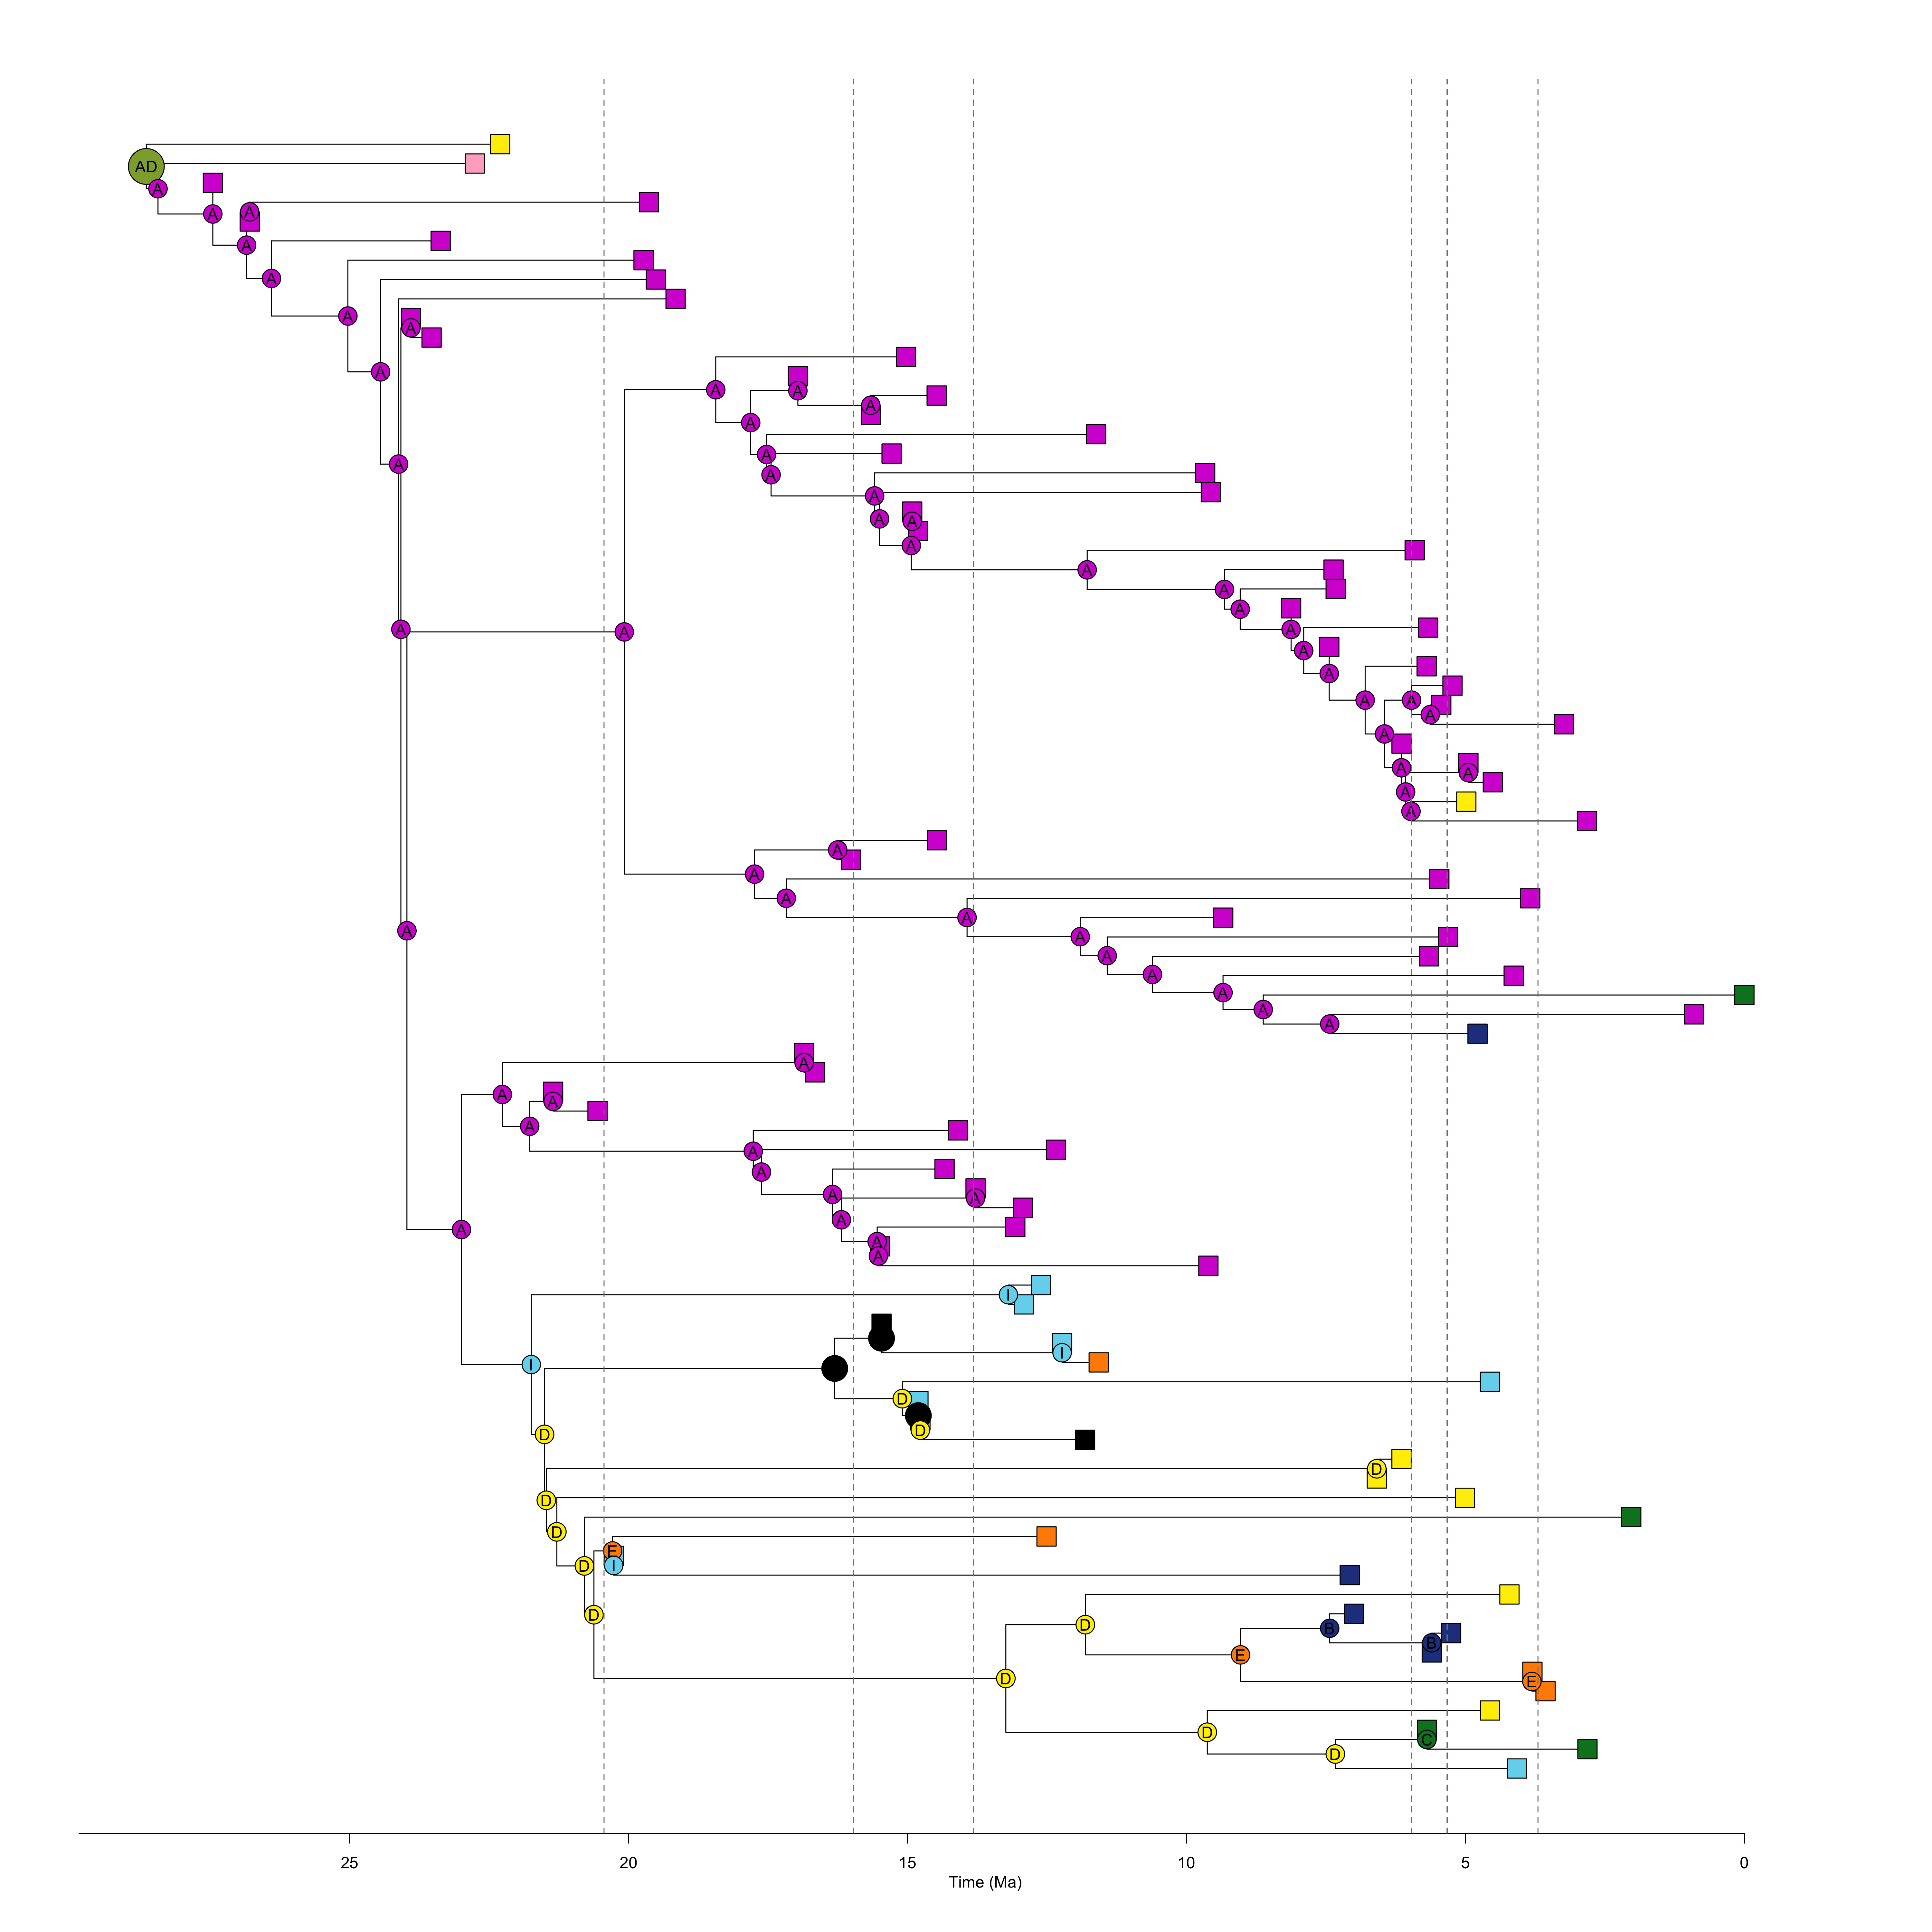
\includegraphics[width = \linewidth]{figures/fossil-pinnipeds-DECj-unlikely-MLstates.png}
%  \caption{Fossil pinnipeds only, DEC+J model, impossible and unlikely states removed. Nodes show Maximum Likelihood states.}
%  \label{fig-fossil-decj-ml-unlikely}
%\end{figure} 

% figure
%\begin{figure}[H]
% \centering
%  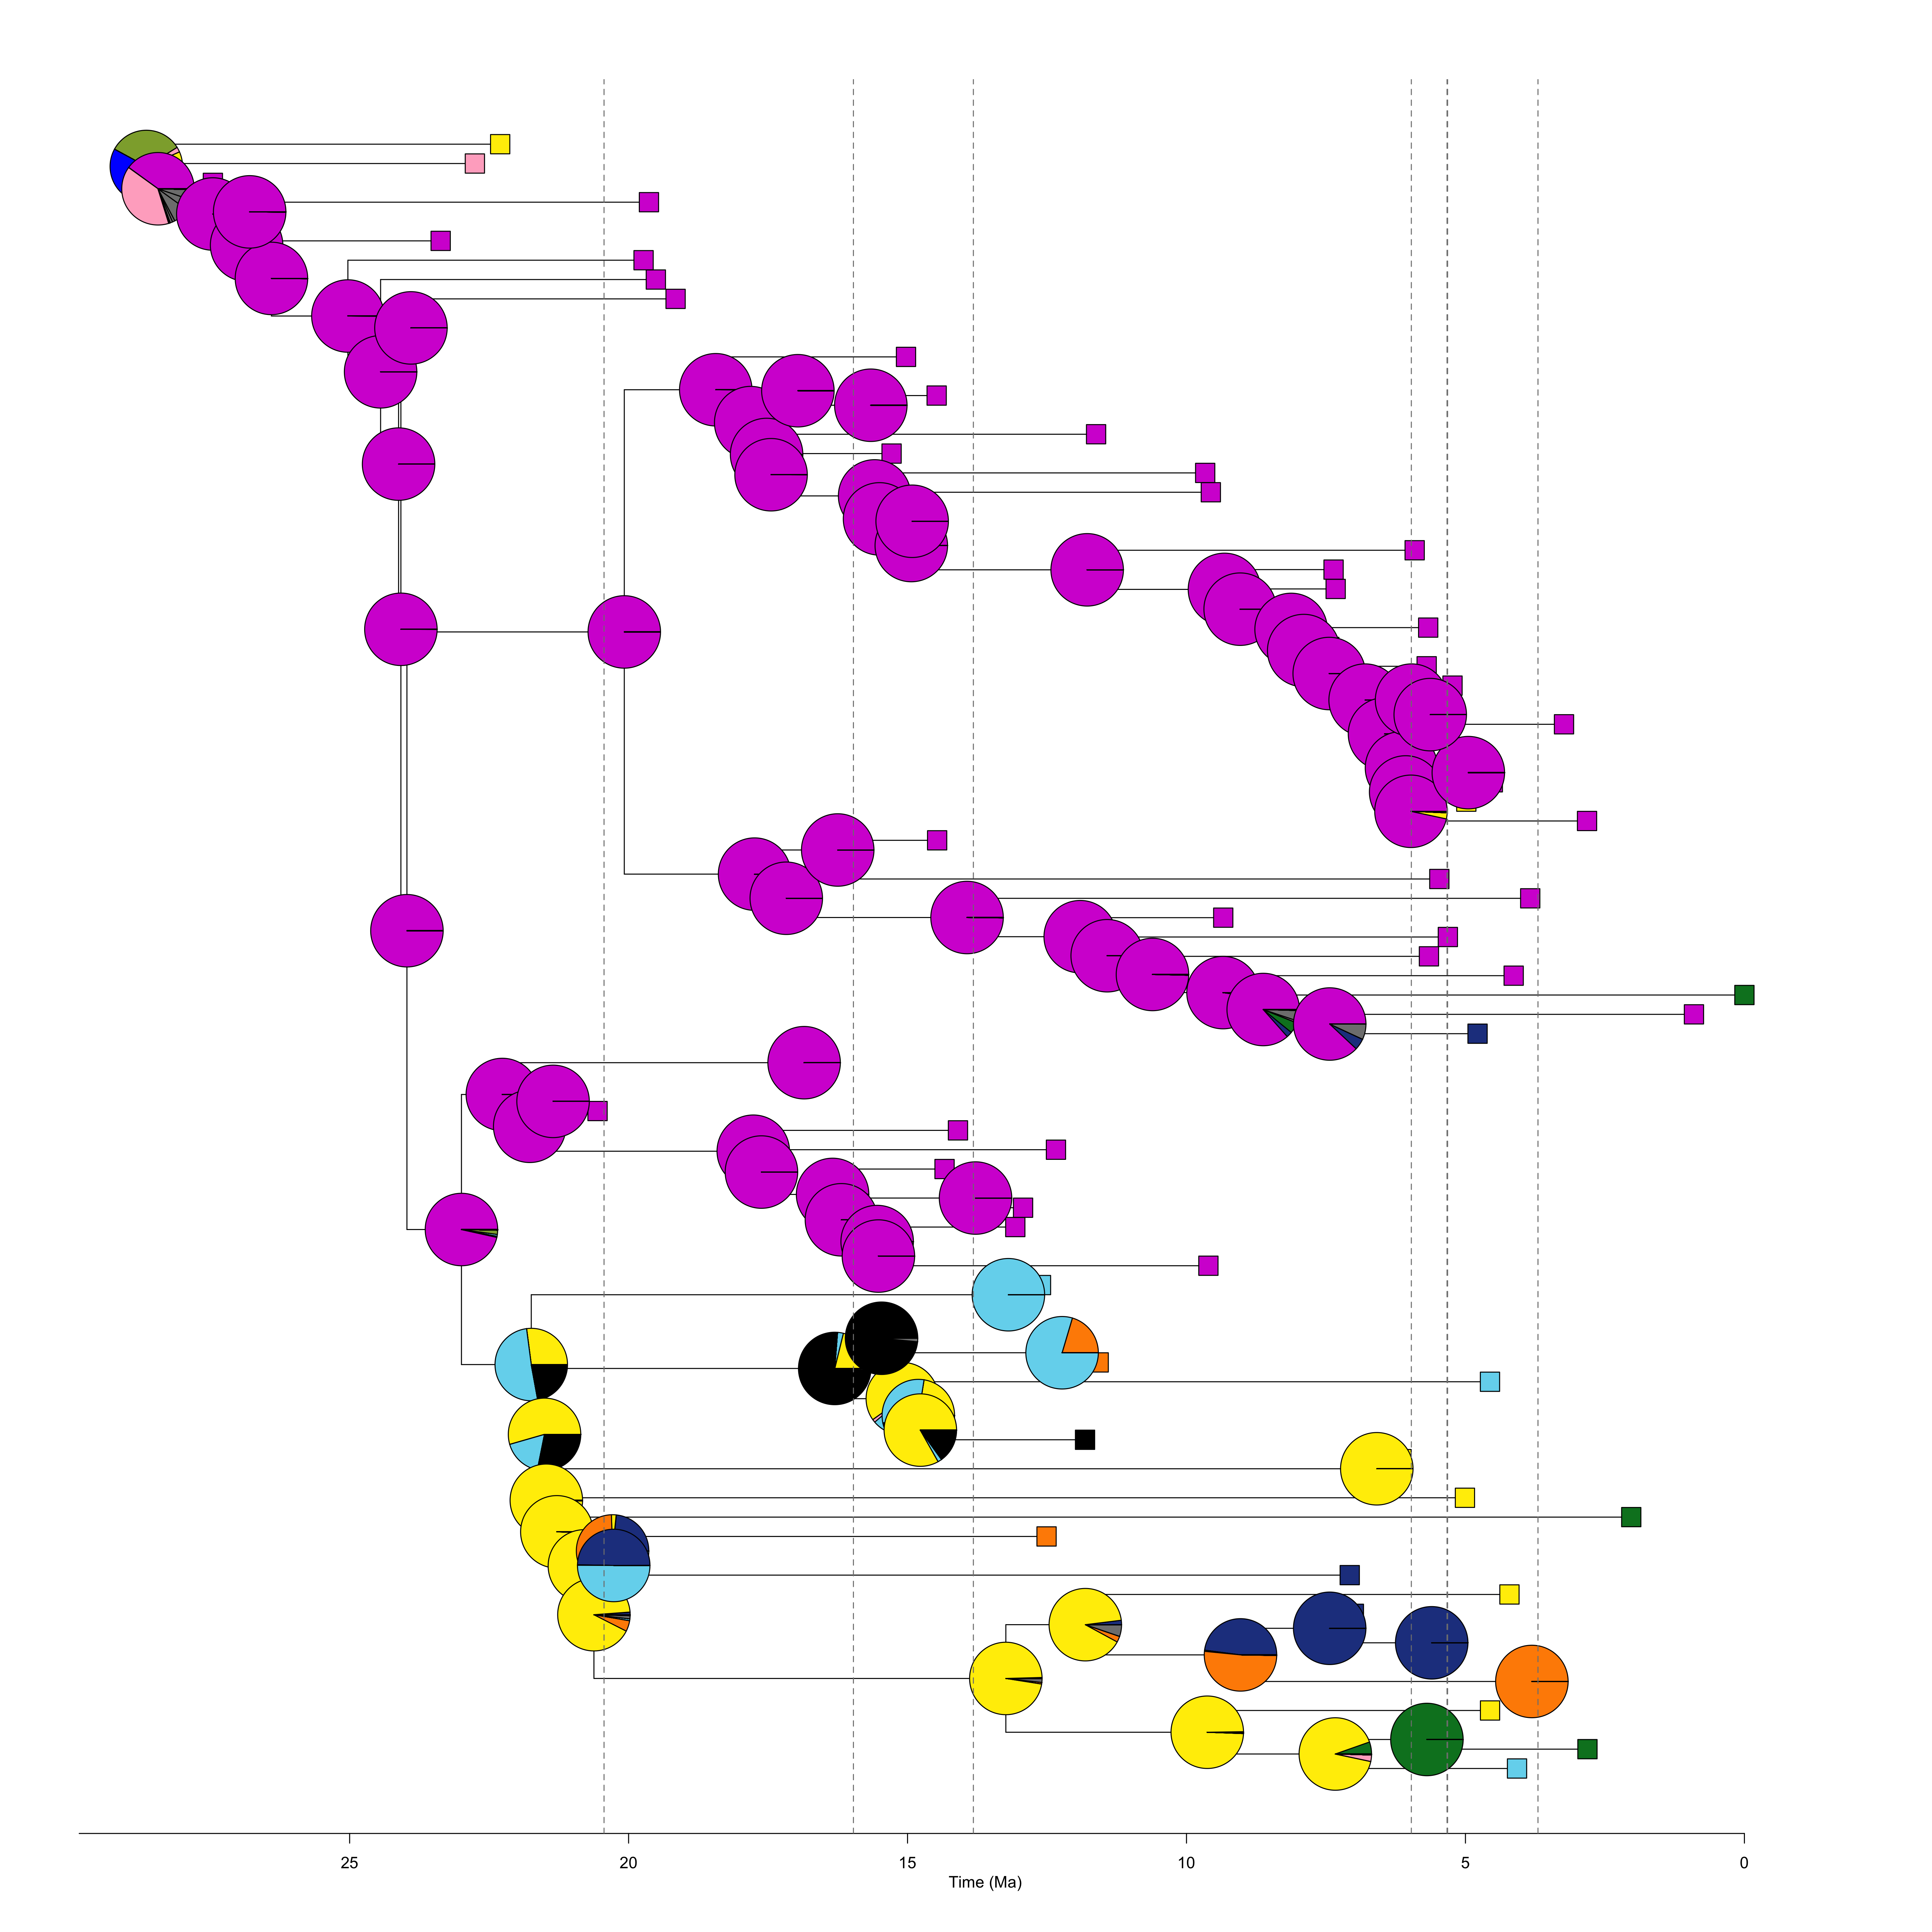
\includegraphics[width = \linewidth]{figures/fossil-pinnipeds-DECj-unlikely-pies.png}
%  \caption{Fossil pinnipeds only, DEC+J model, impossible and unlikely states removed. Nodes show relative probabilities of each state.}
%  \label{fig-fossil-decj-pie-unlikely}
%\end{figure} 
%-----------------------------------------------------------------------------------
\subsubsection{Extant pinnipeds only}

% figure
%\begin{figure}[H]
% \centering
%  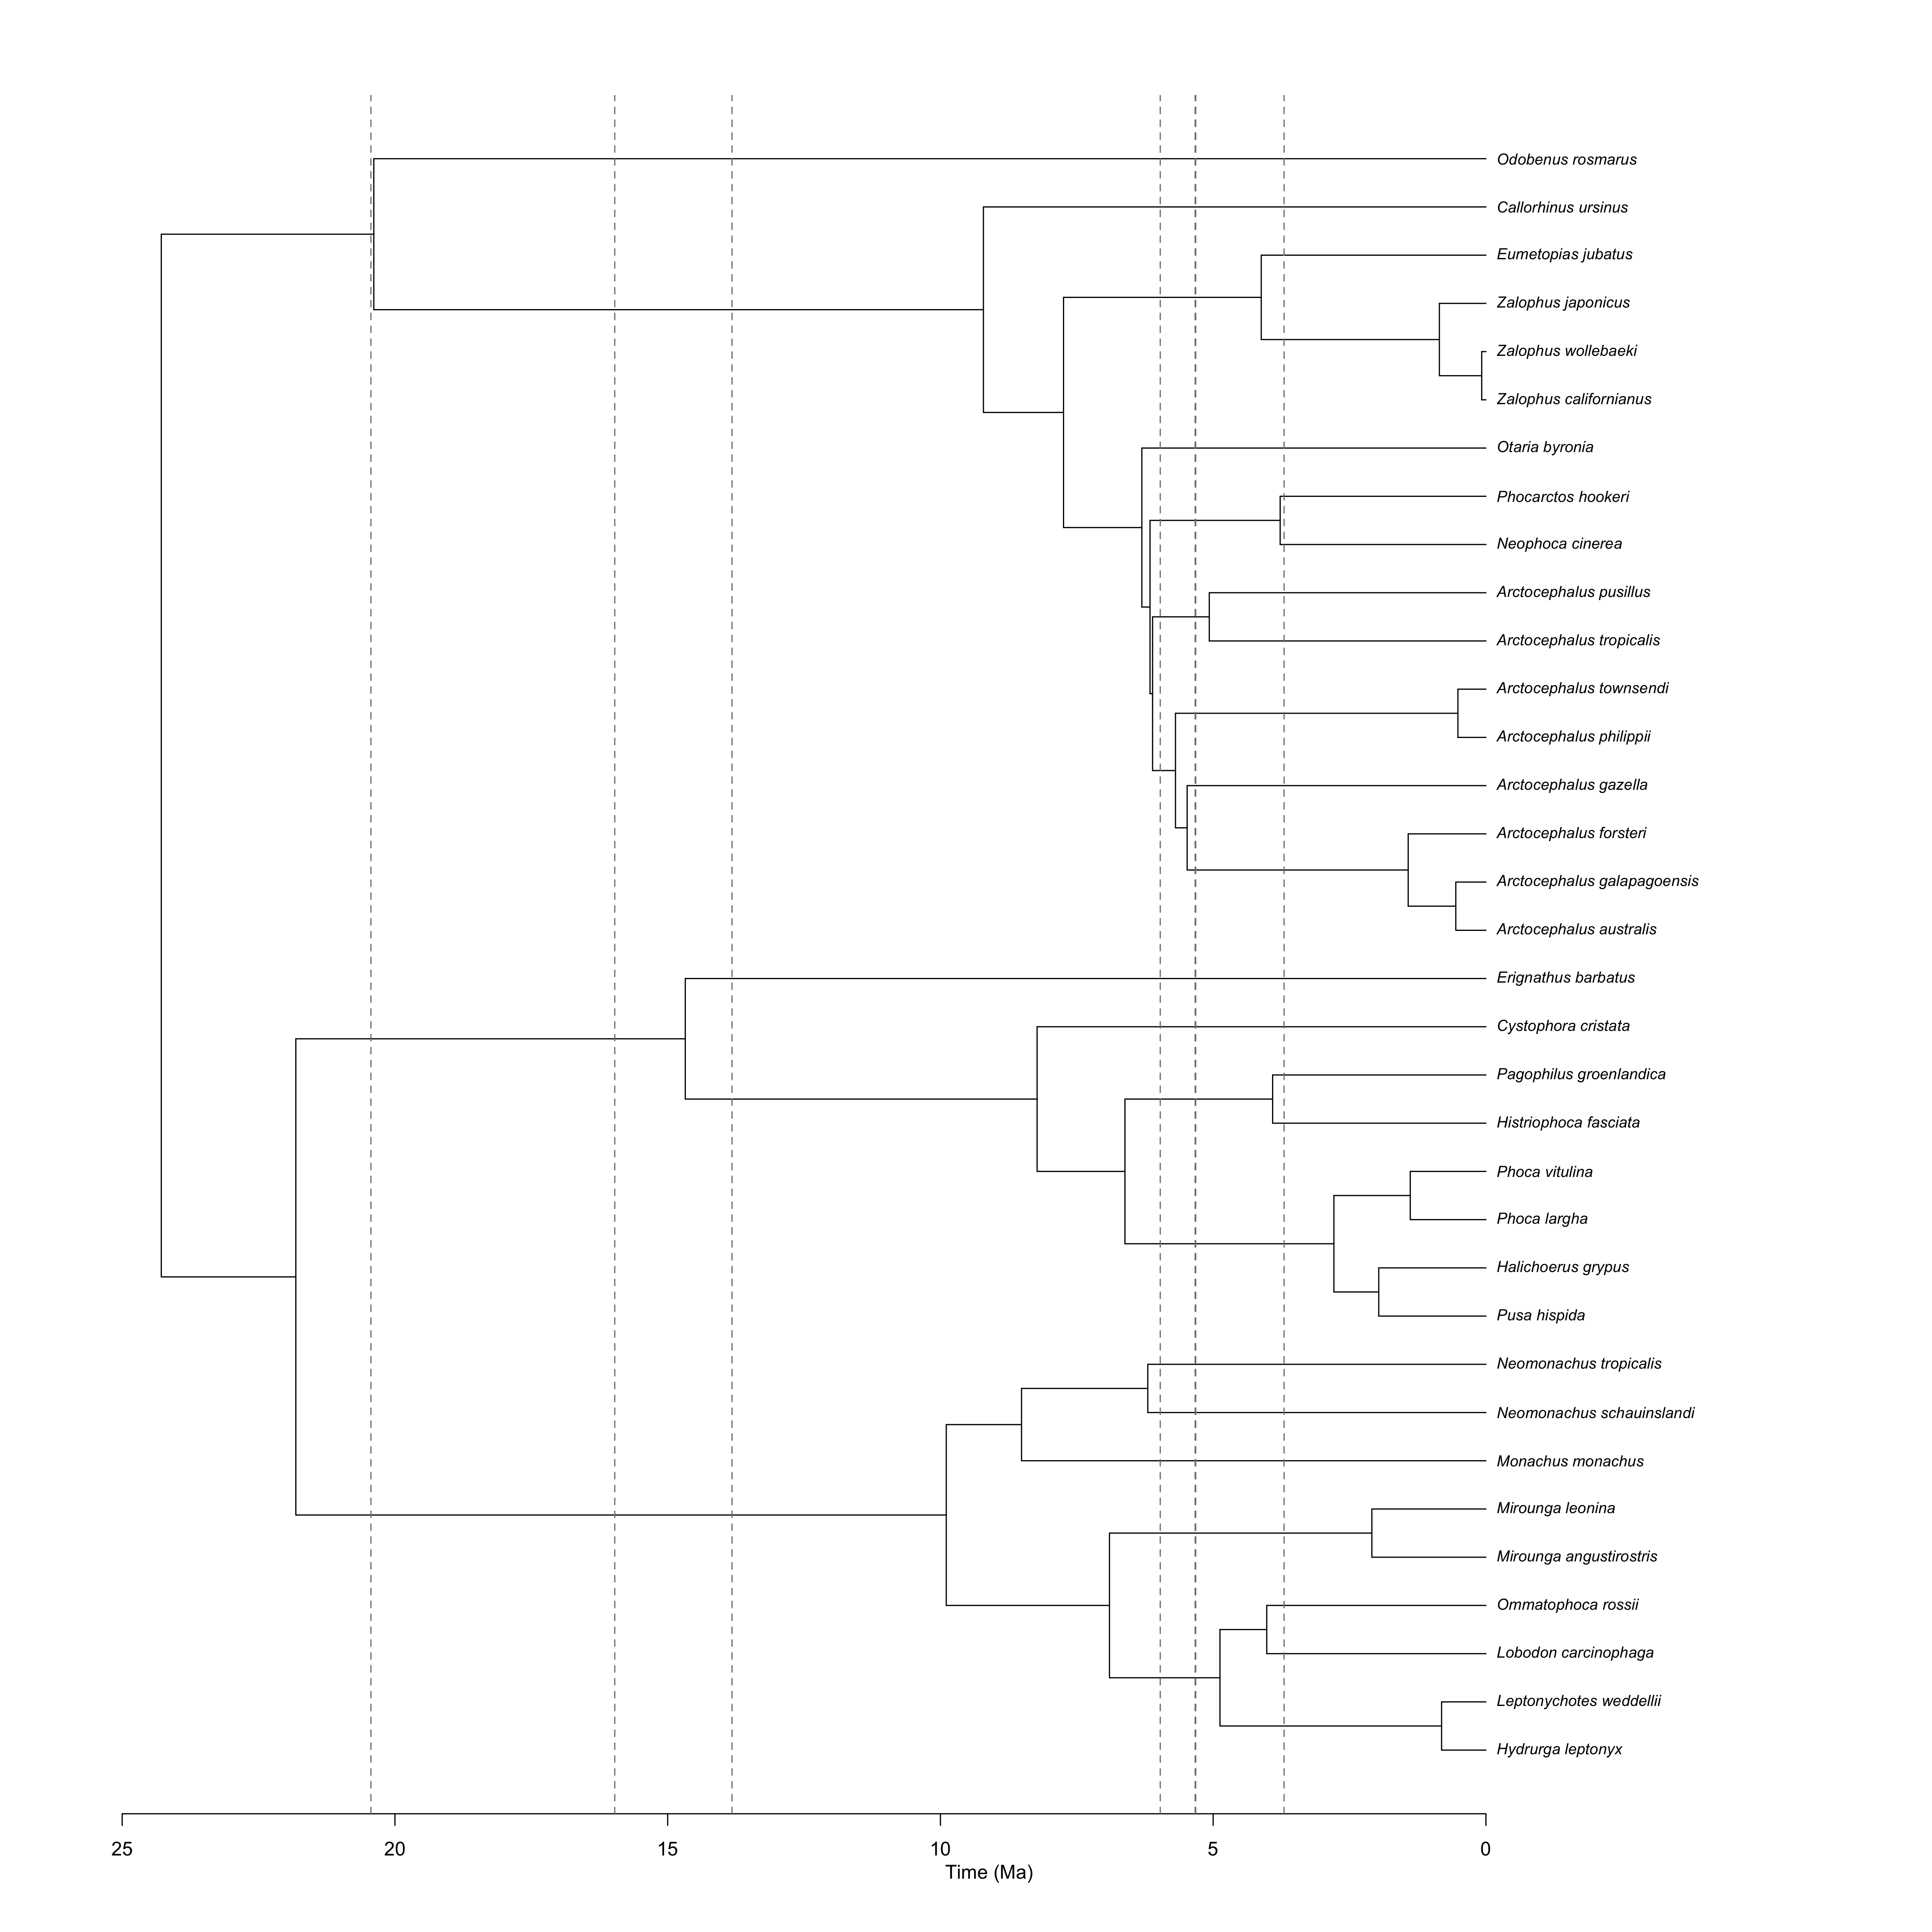
\includegraphics[width = \linewidth]{figures/extant-pinnipeds-tree.png}
%  \caption{Phylogeny of extant pinnipeds with taxon names to aid understanding of the following results which have taxon names removed to improve readability.}
%  \label{fig-extant-tree}
%\end{figure} 

% figure
%\begin{figure}[H]
% \centering
%  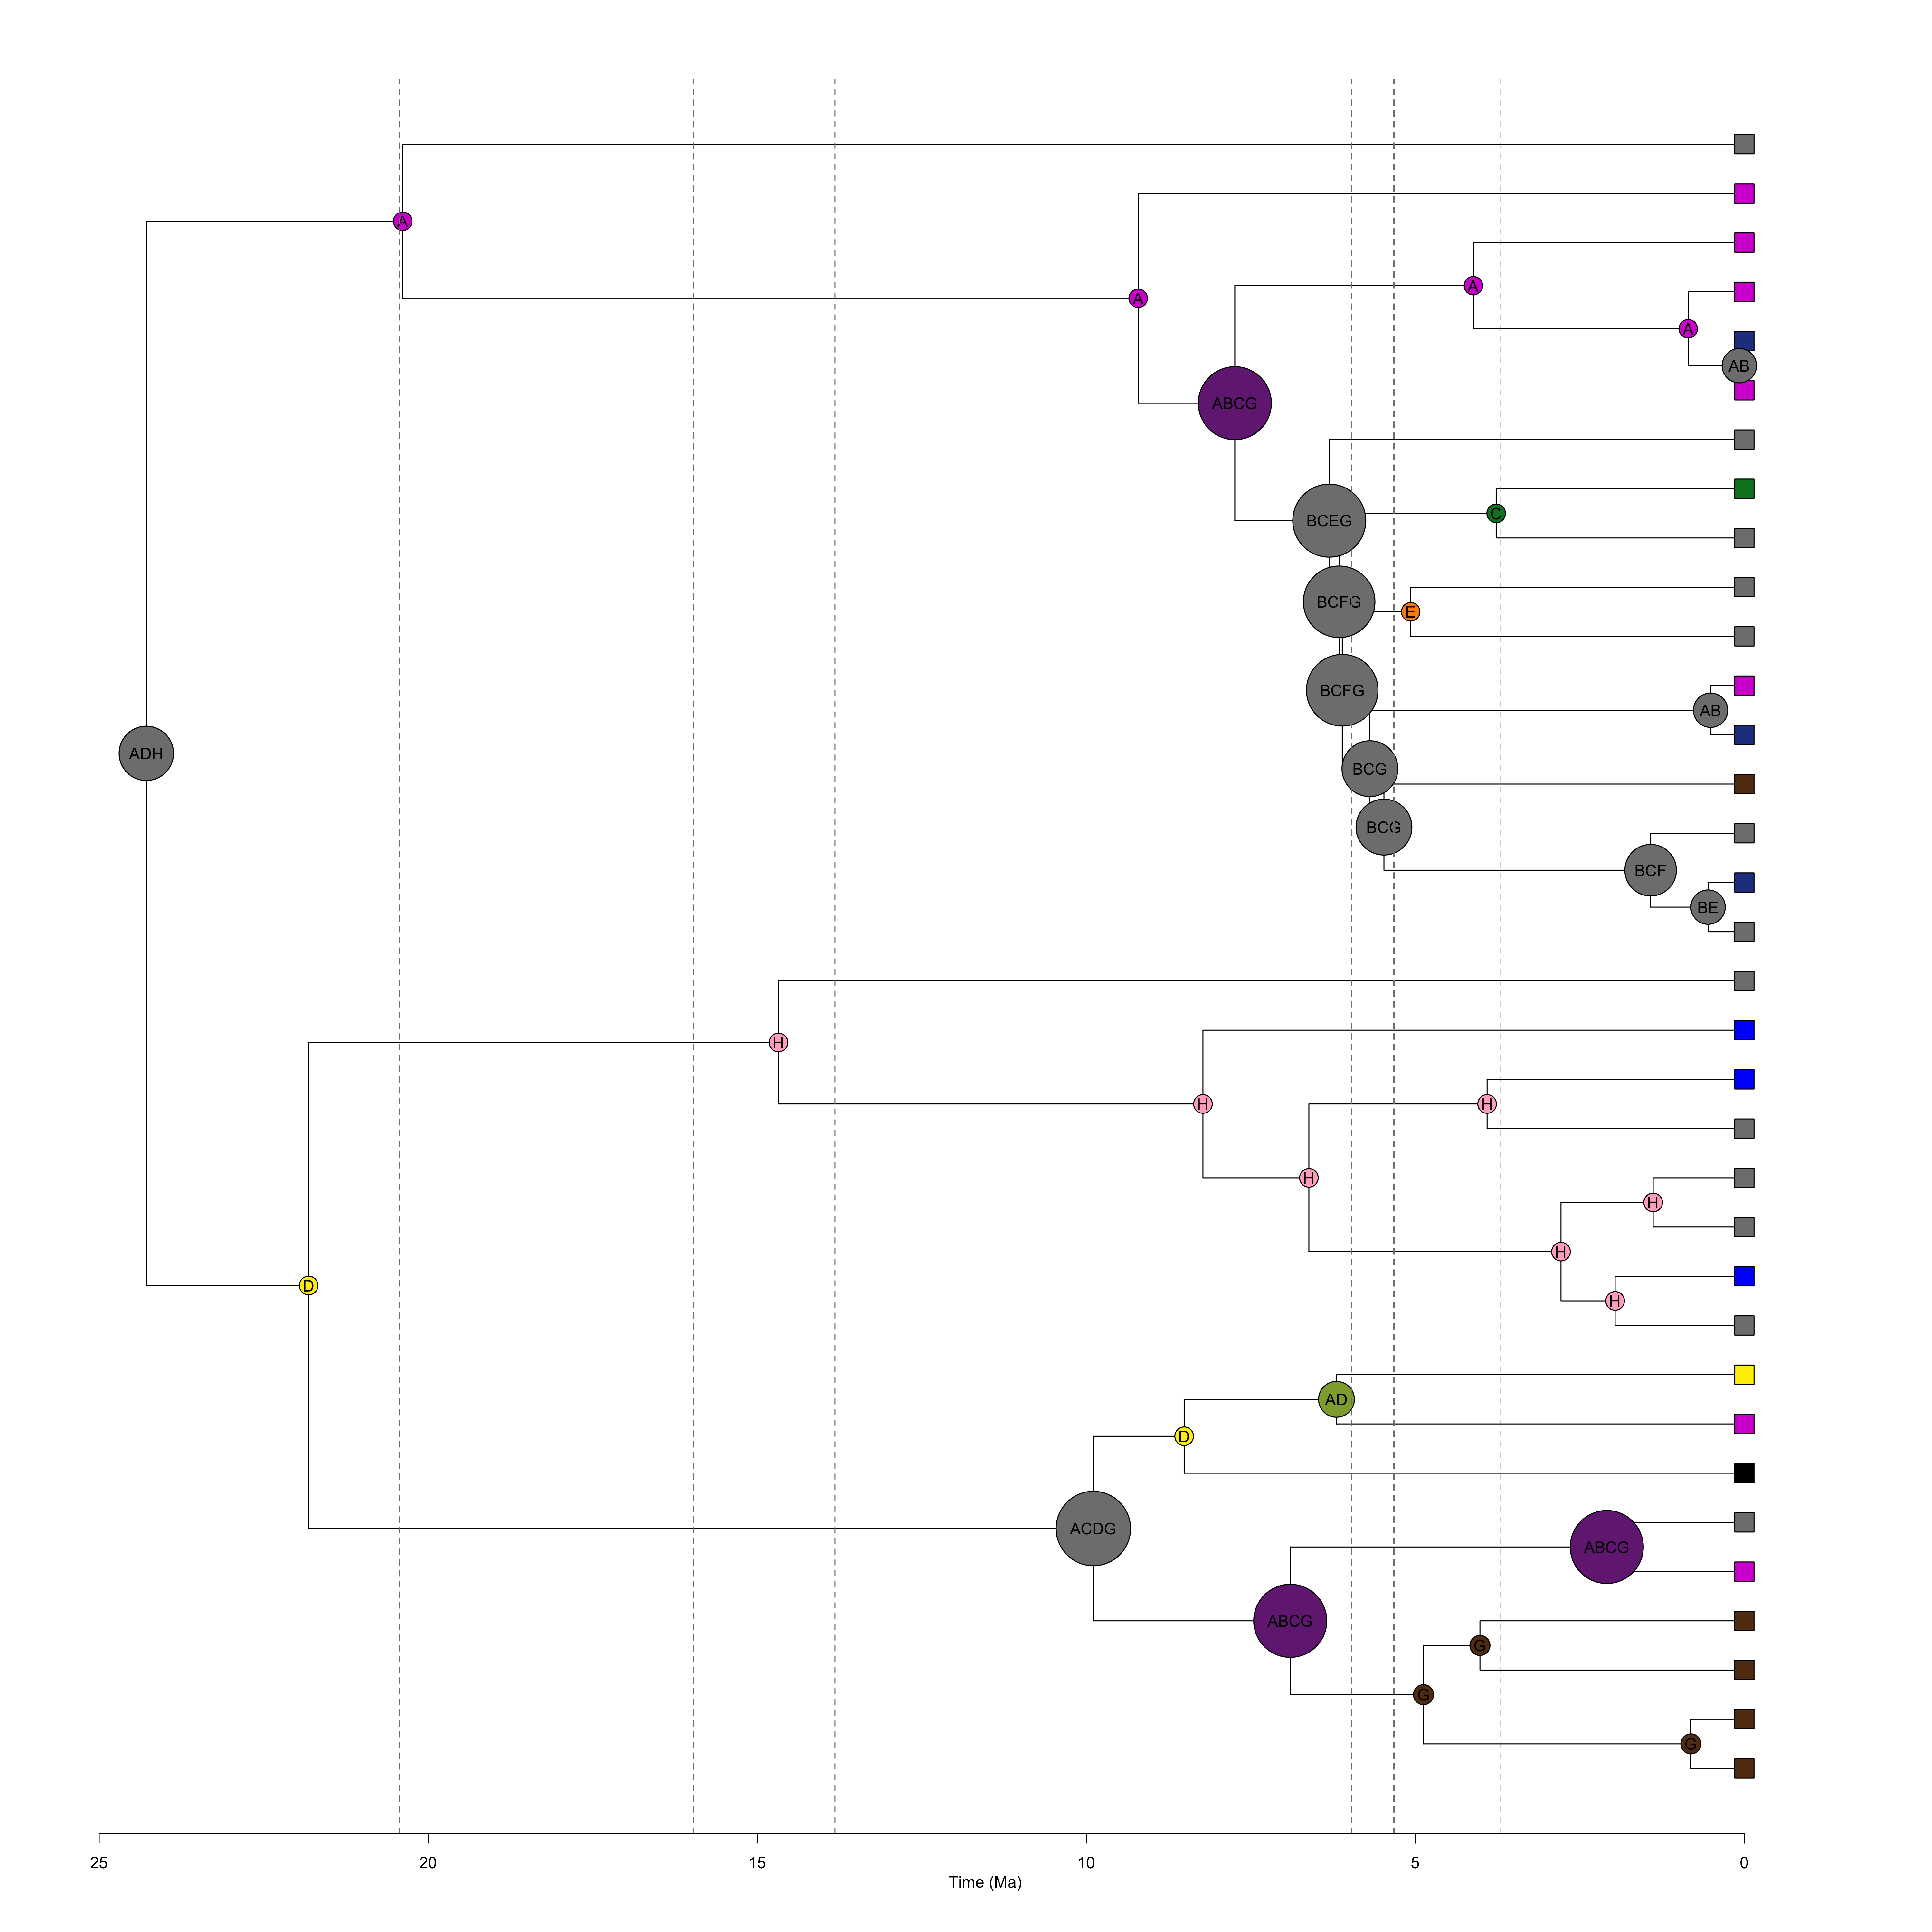
\includegraphics[width = \linewidth]{figures/extant-pinnipeds-DEC-impossible-MLstates.png}
%  \caption{Extant pinnipeds only, DEC model, impossible states removed. Nodes show Maximum Likelihood states.}
%  \label{fig-extant-dec-ml}
%\end{figure} 

% figure
%\begin{figure}[H]
% \centering
%  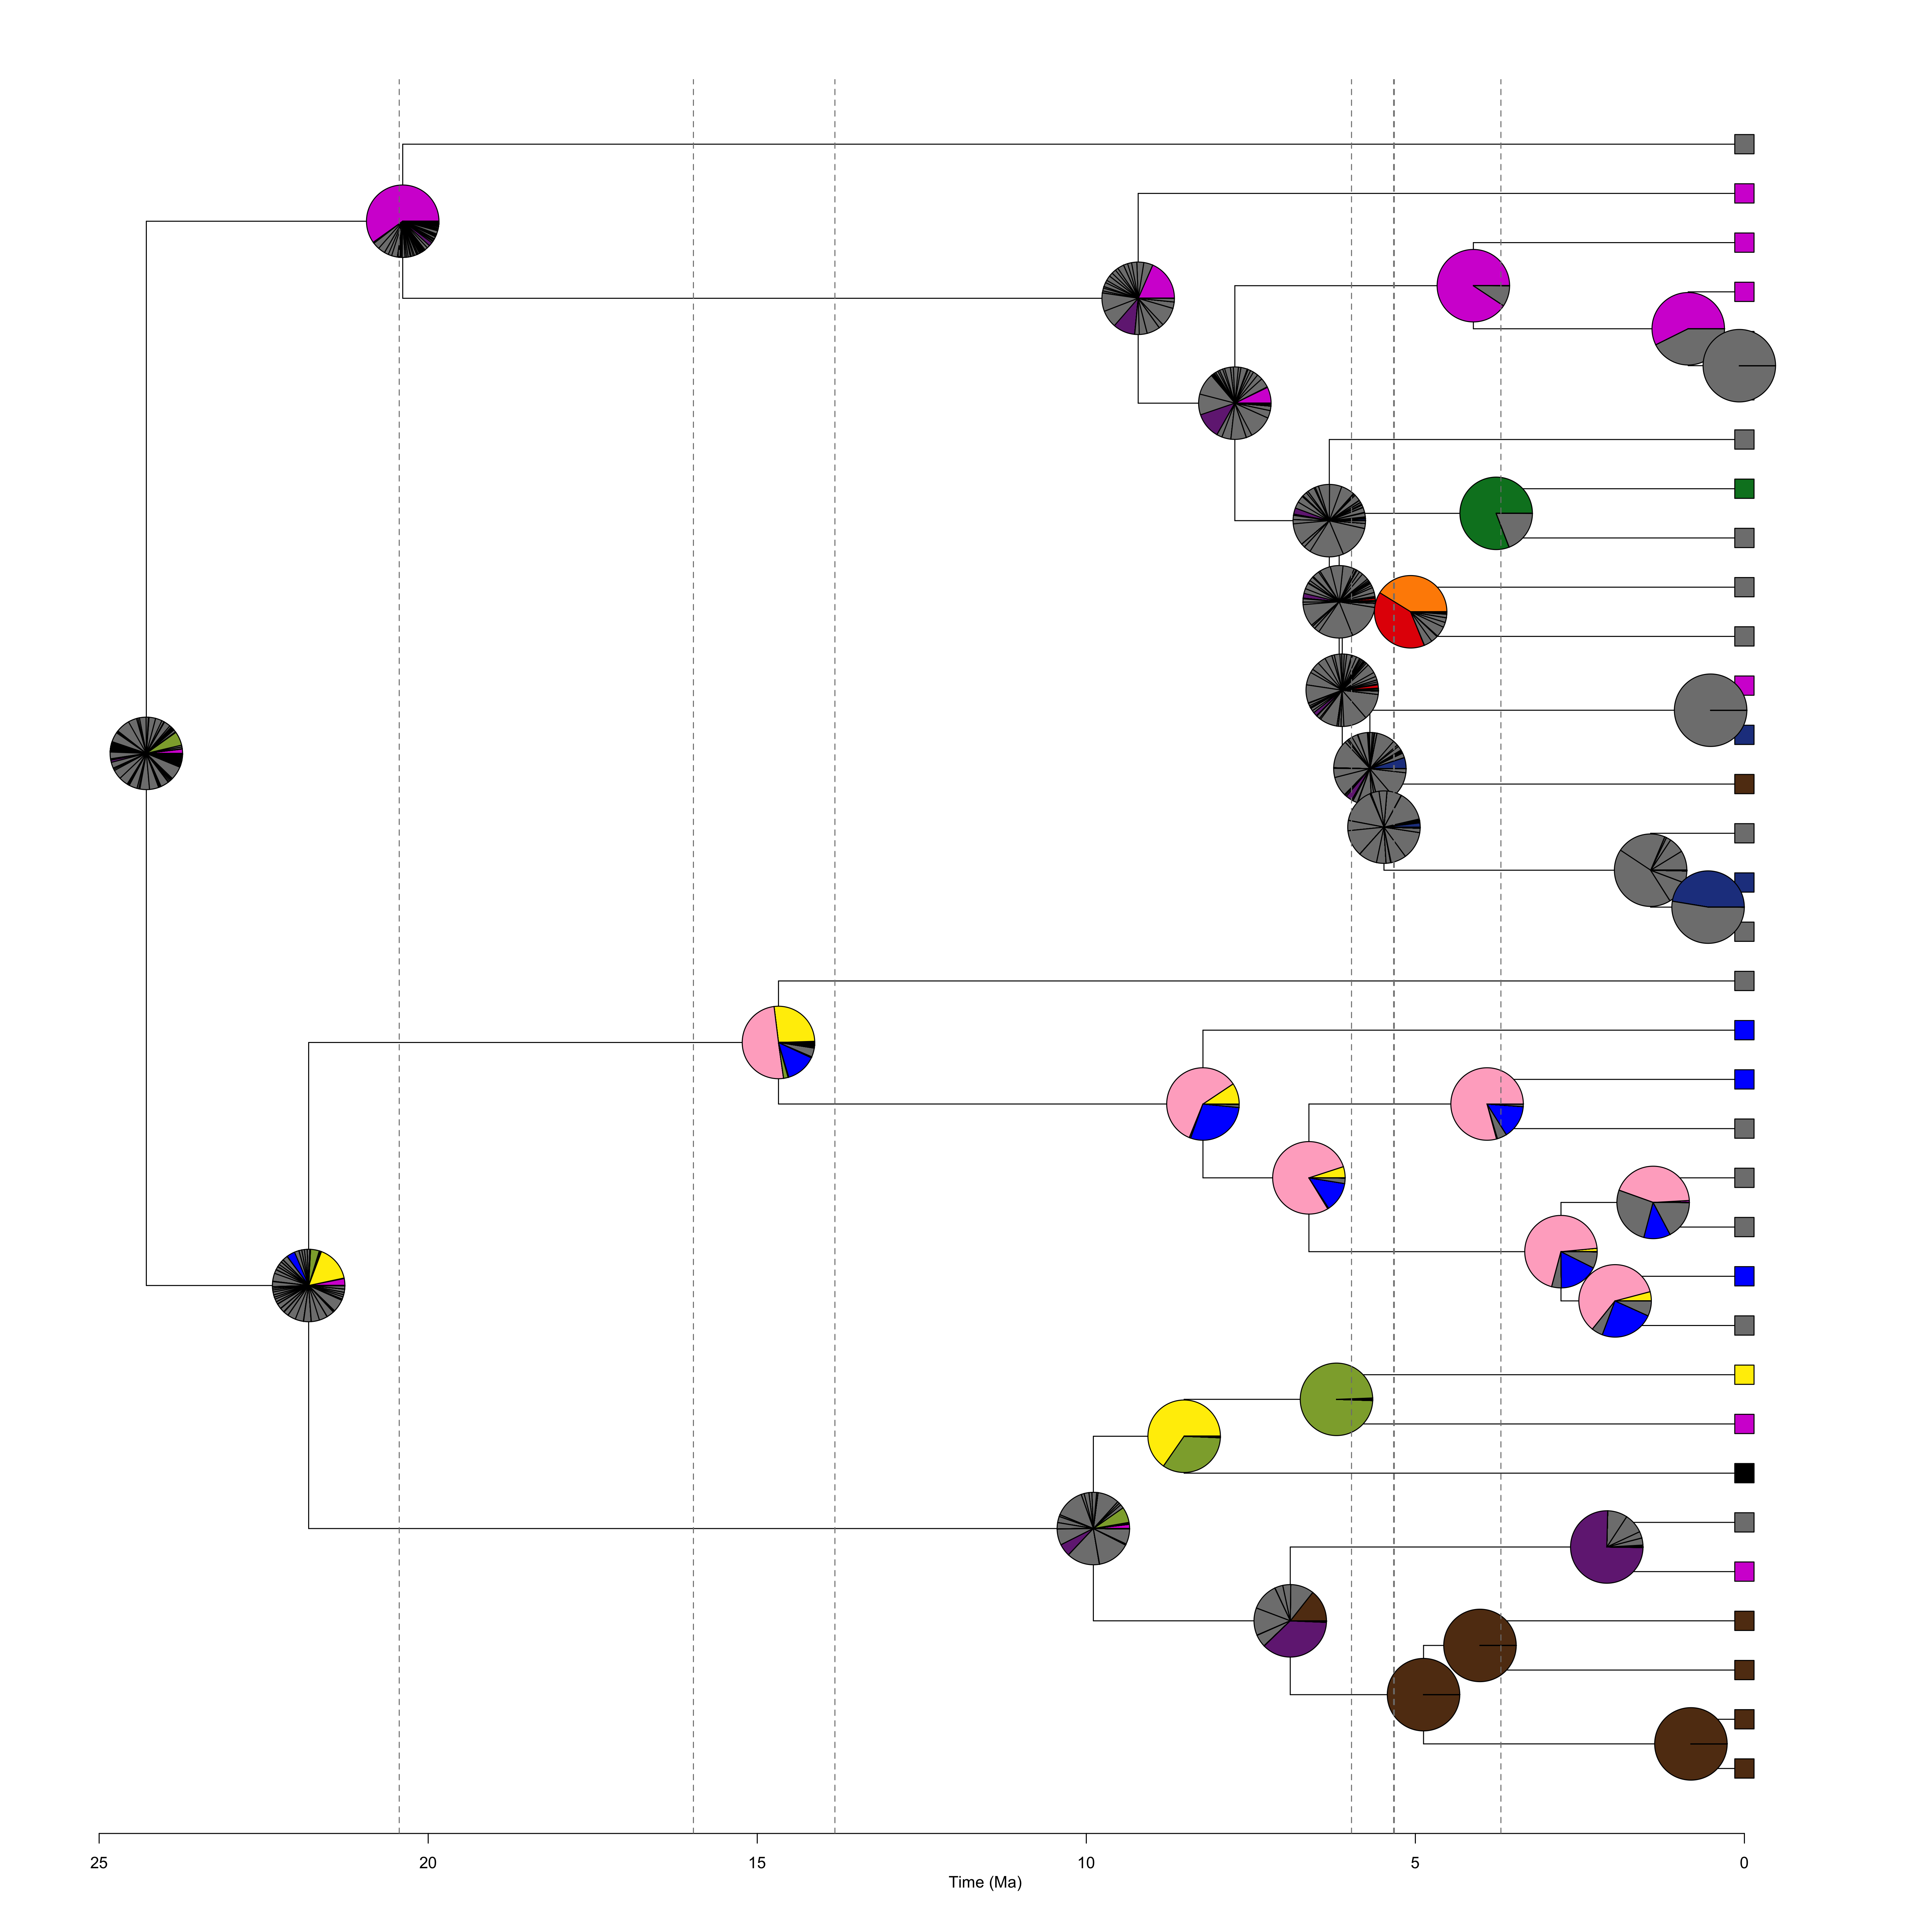
\includegraphics[width = \linewidth]{figures/extant-pinnipeds-DEC-impossible-pies.png}
 % \caption{Extant pinnipeds only, DEC model, impossible states removed. Nodes show relative probabilities of each state.}
%  \label{fig-extant-dec-pie}
%\end{figure} 

% figure
%\begin{figure}[H]
% \centering
 % 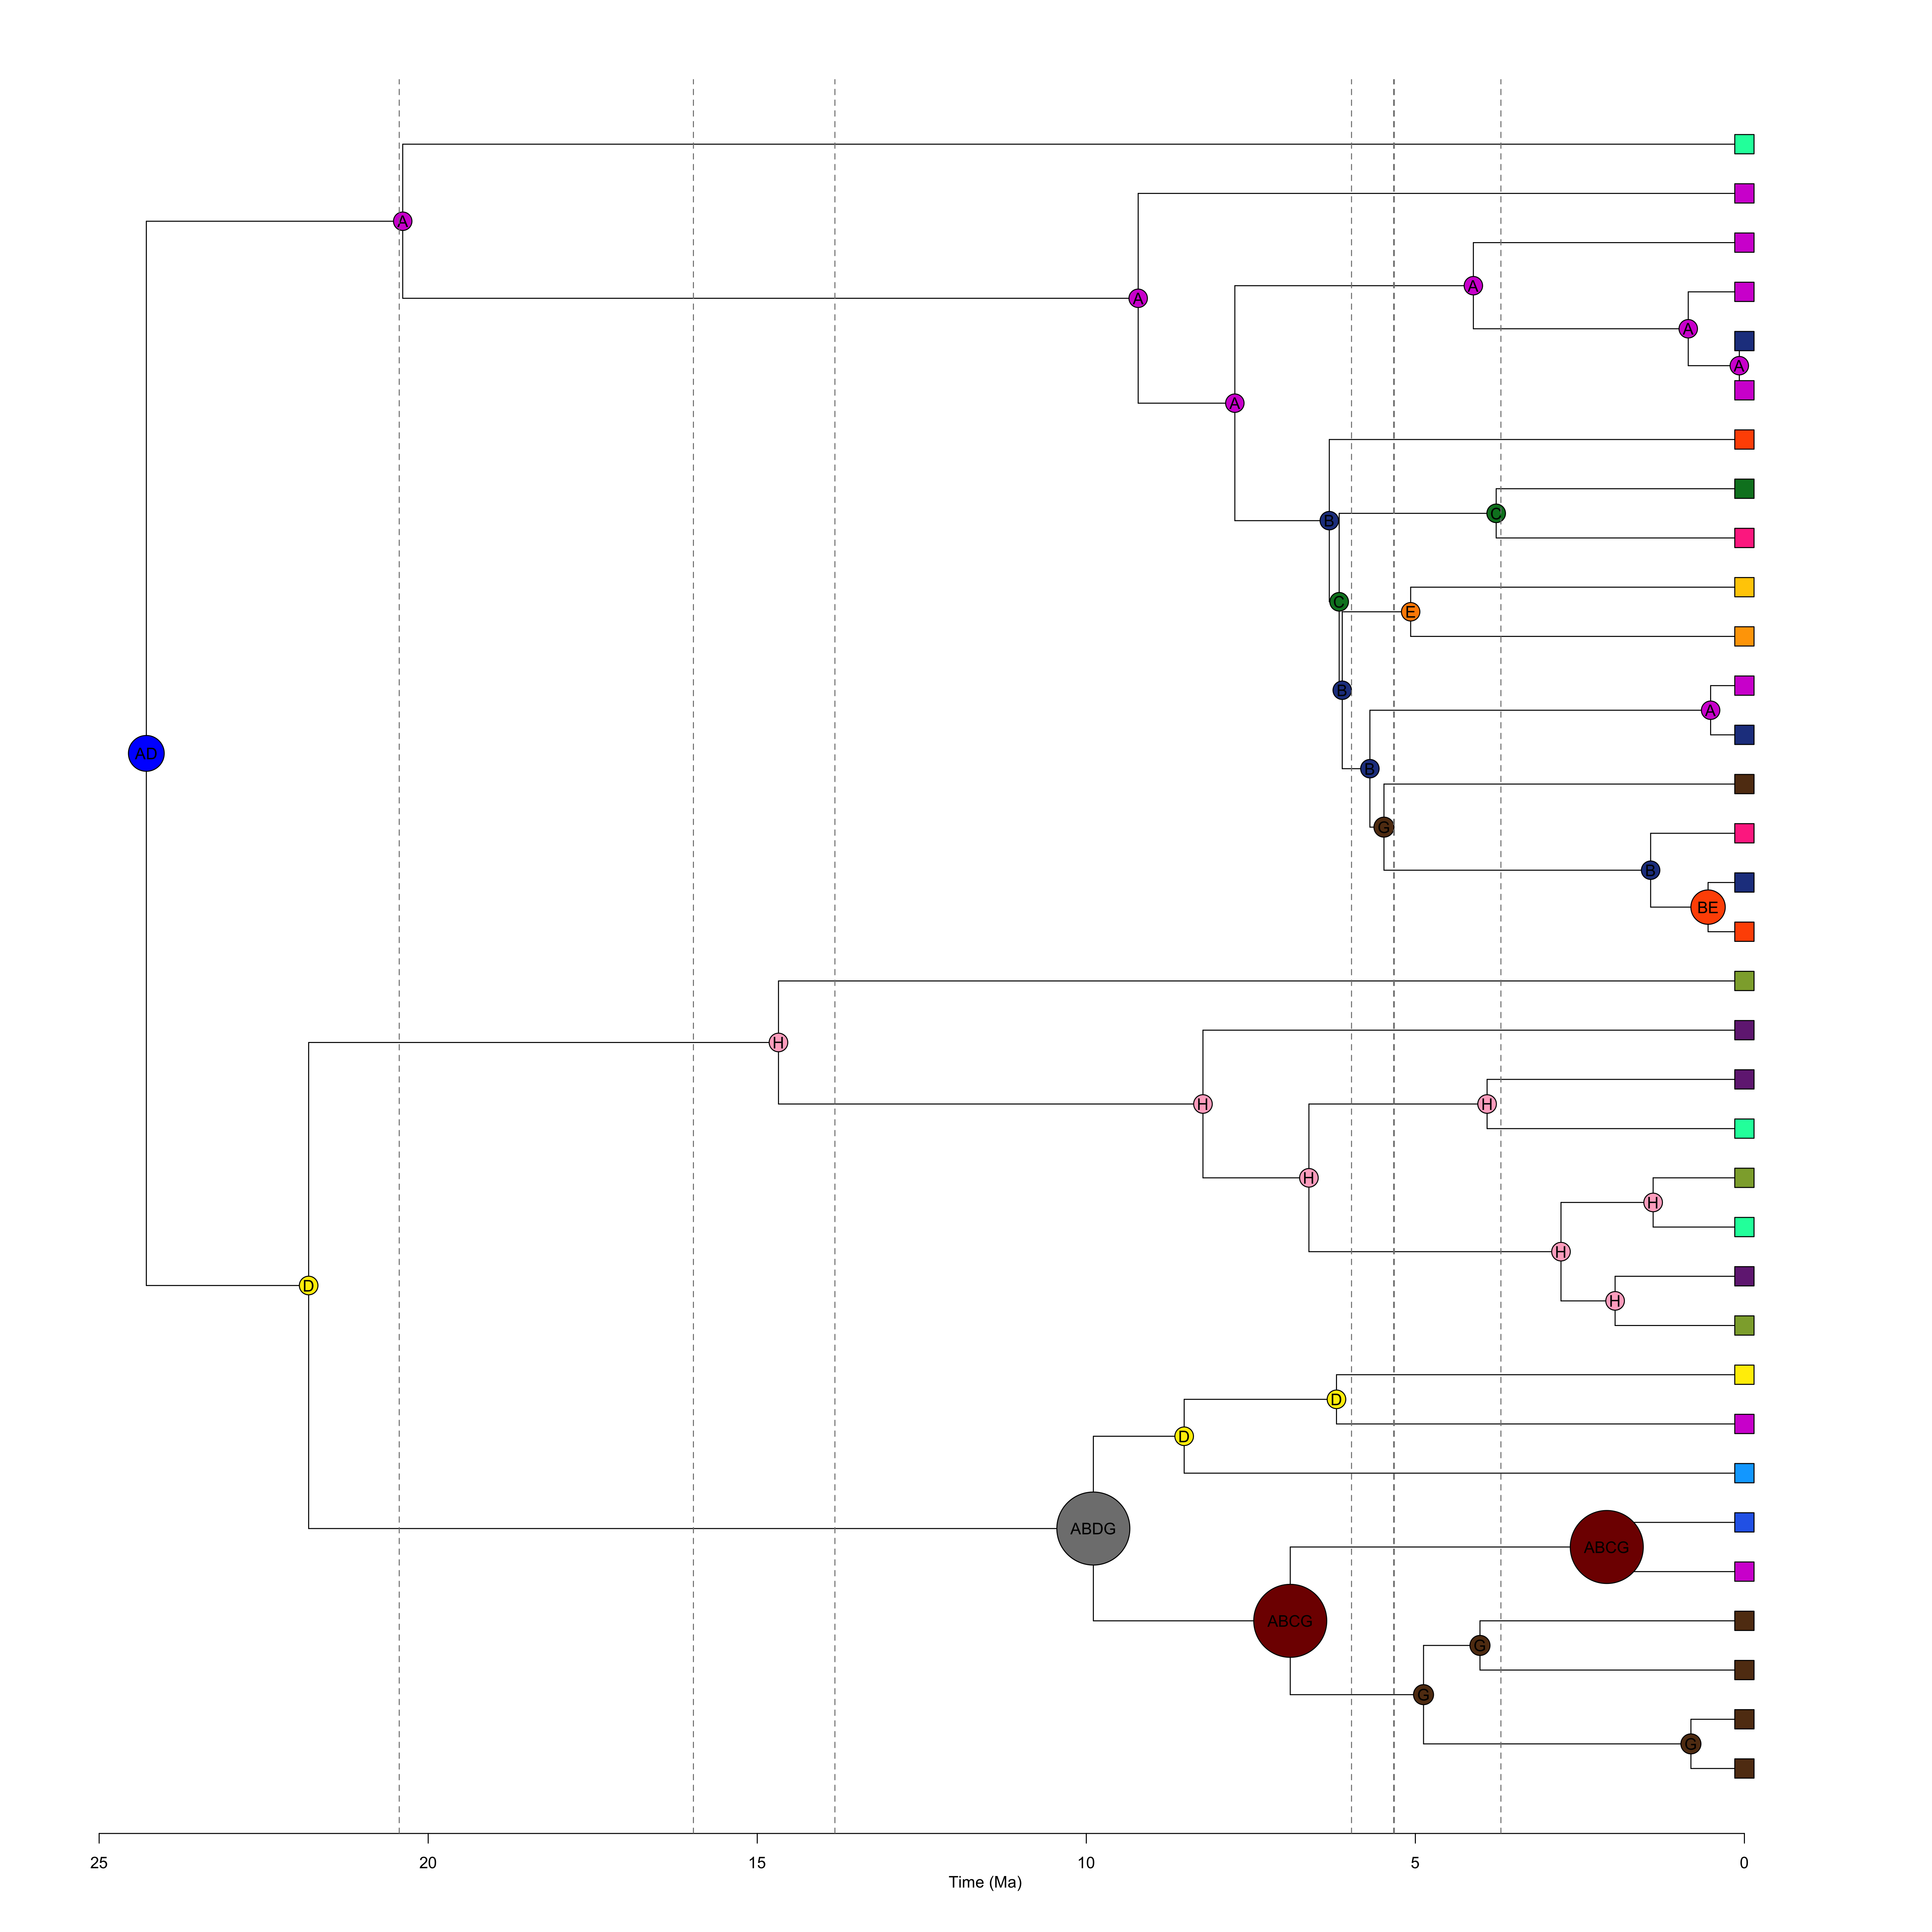
\includegraphics[width = \linewidth]{figures/extant-pinnipeds-DECj-impossible-MLstates.png}
 % \caption{Extant pinnipeds only, DEC+J model, impossible states removed. Nodes show Maximum Likelihood states.}
 % \label{fig-extant-decj-ml}
%\end{figure} 

% figure
%\begin{figure}[H]
% \centering
 % 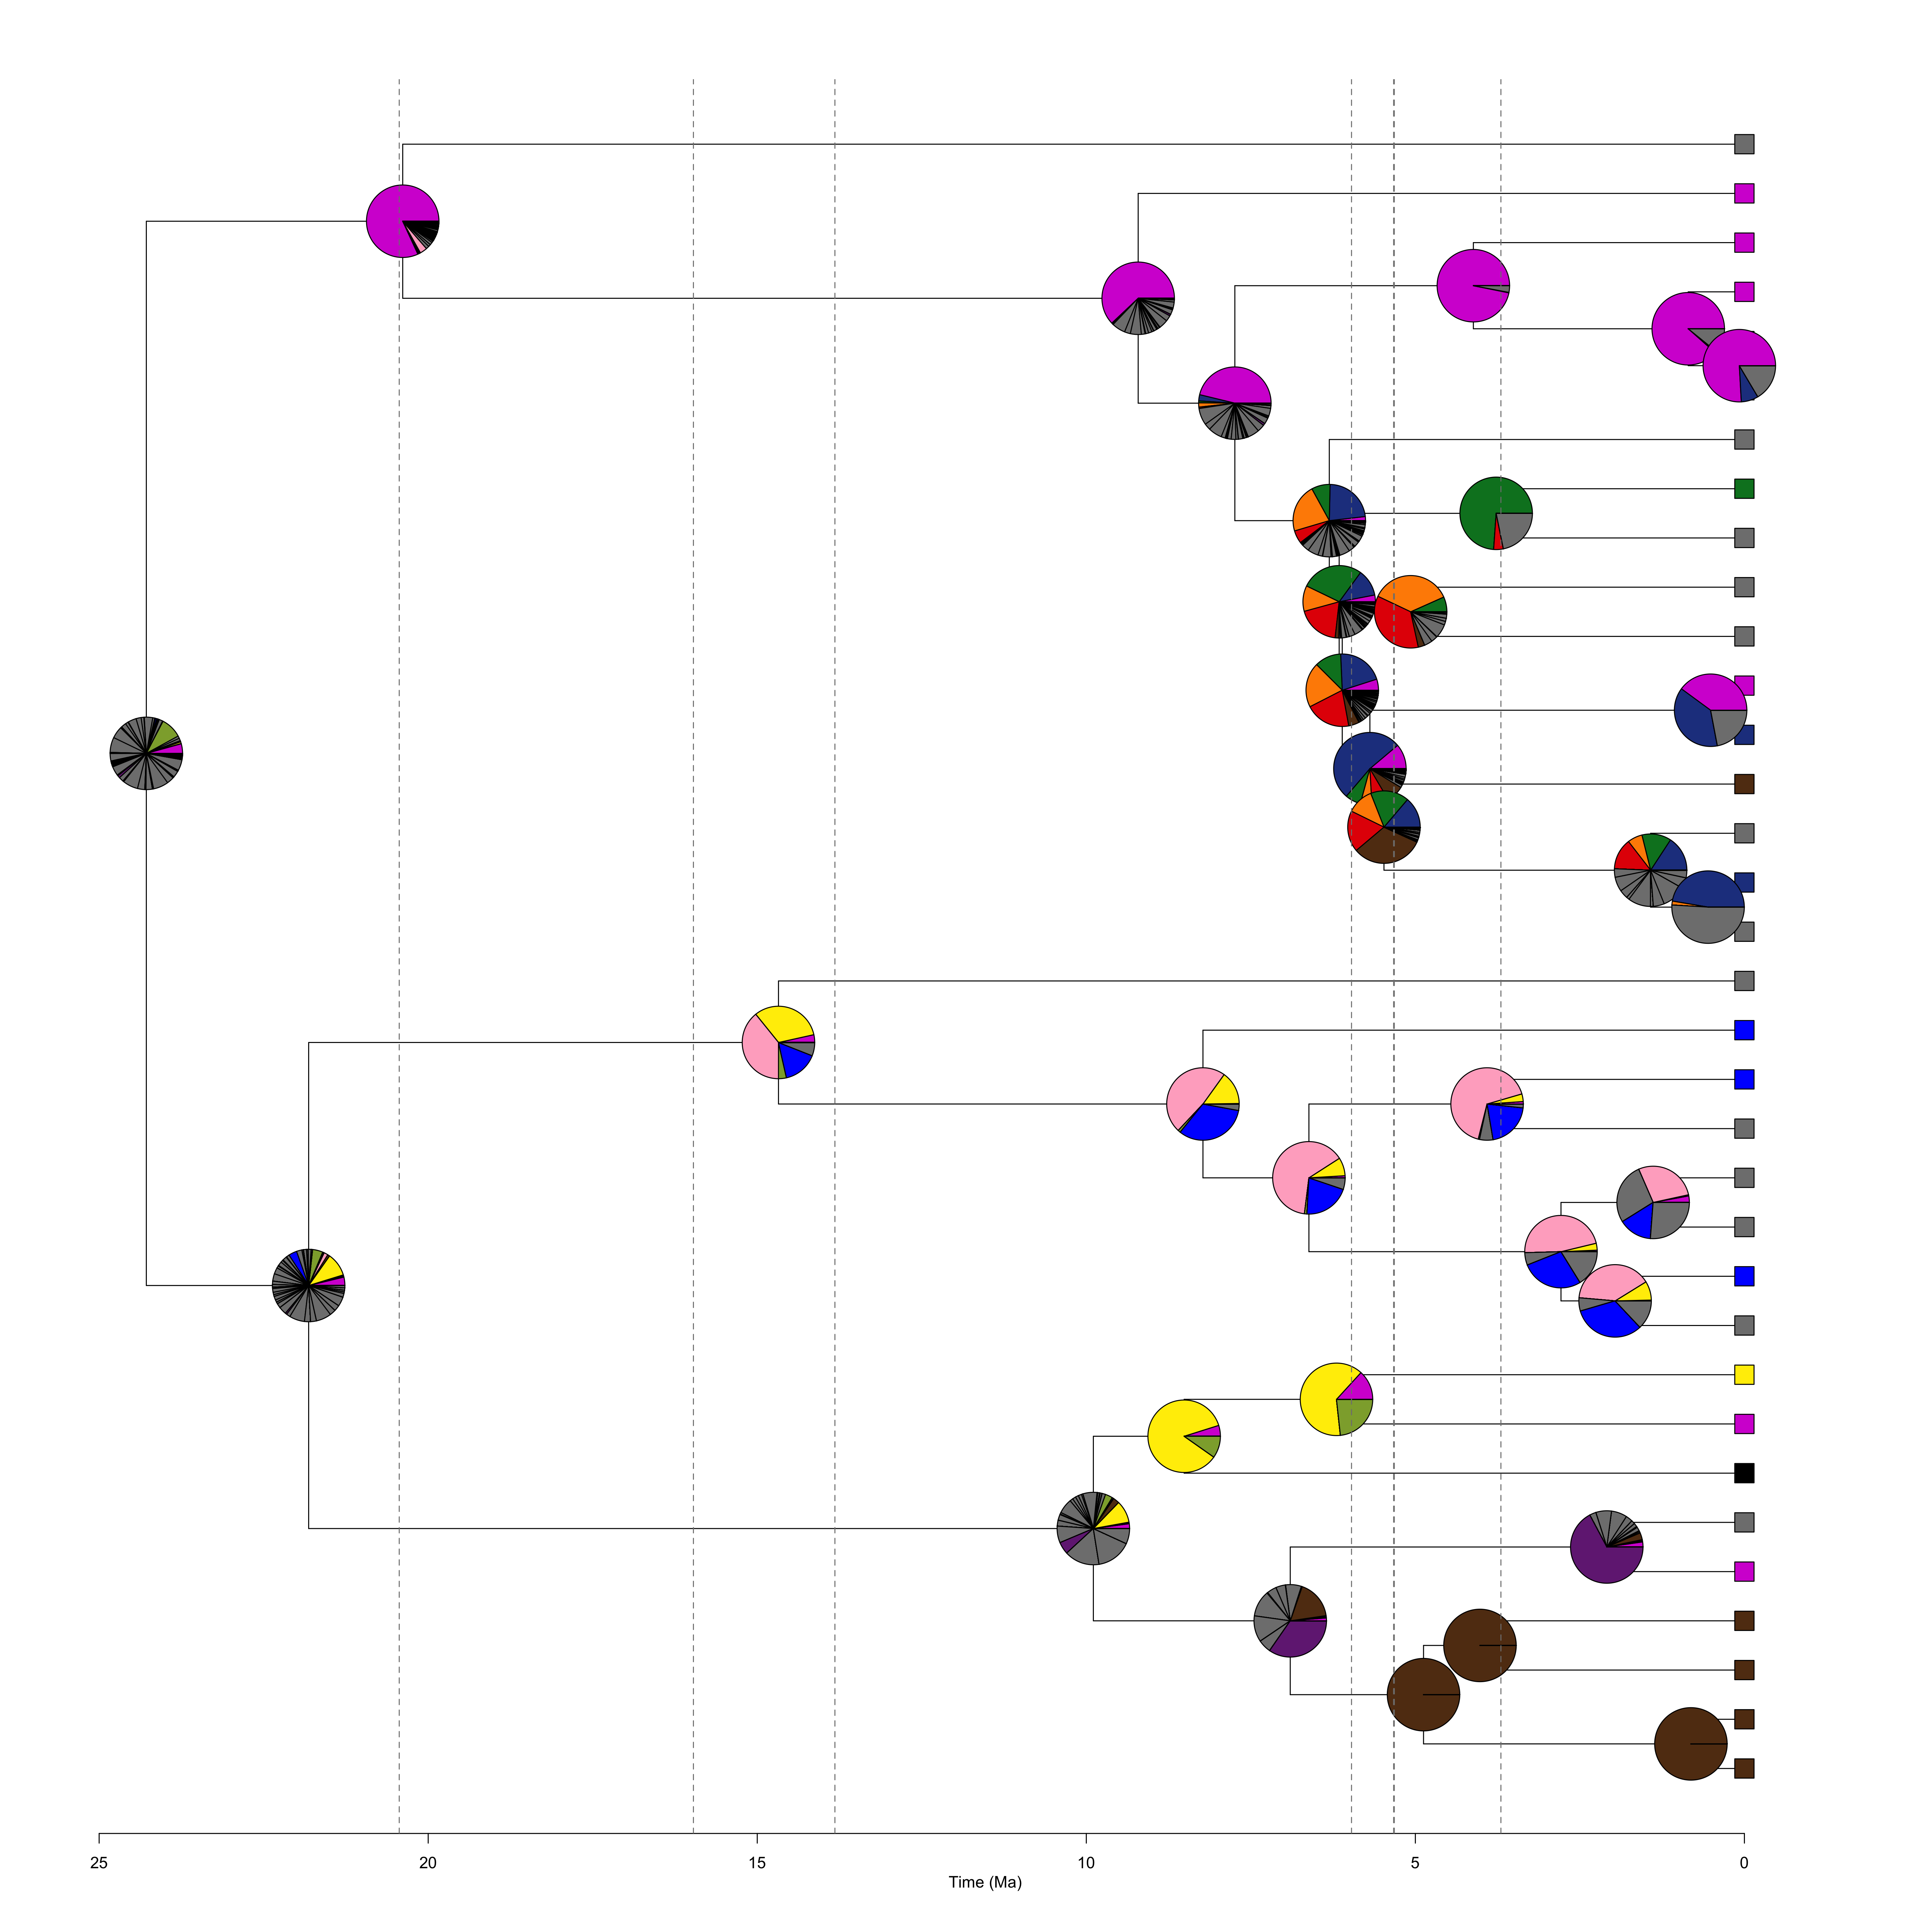
\includegraphics[width = \linewidth]{figures/extant-pinnipeds-DECj-impossible-pies.png}
 % \caption{Extant pinnipeds only, DEC+J model, impossible states removed. Nodes show relative probabilities of each state.}
 % \label{fig-extant-decj-pie}
%\end{figure} 
 
%-----------------------------------------------------------------------------------
% unlikely + extant

% figure
%\begin{figure}[H]
% \centering
%  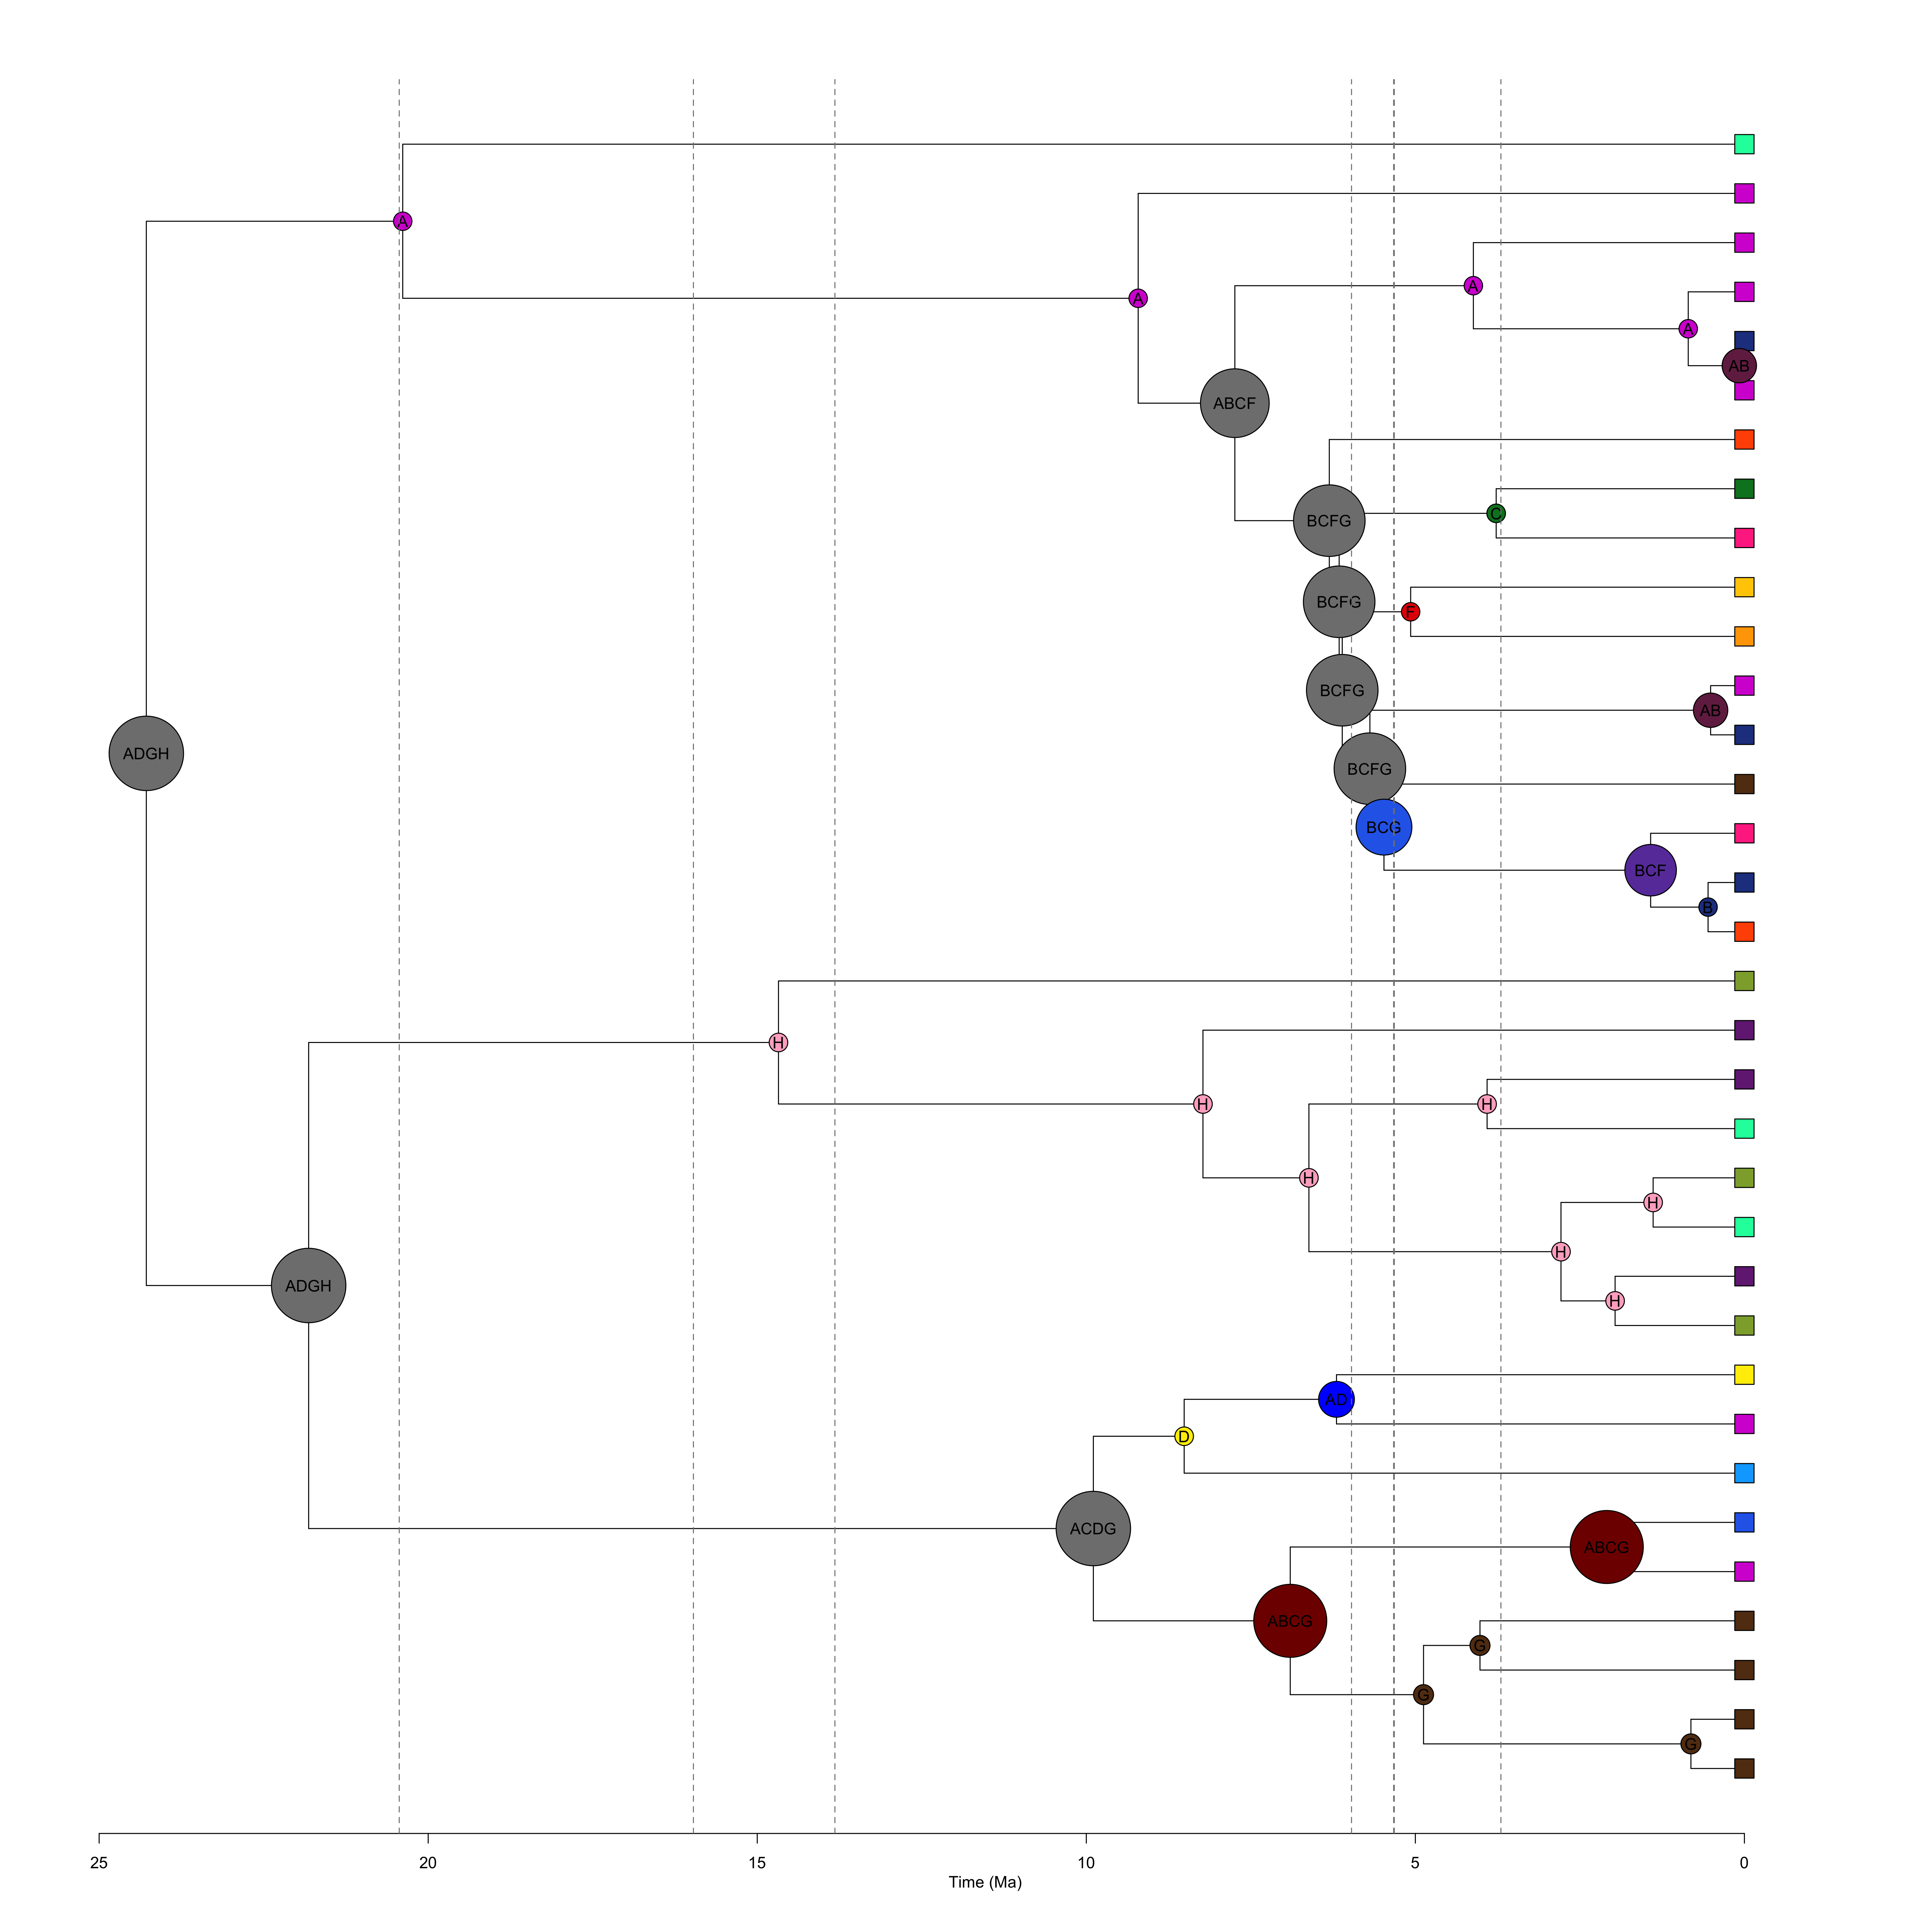
\includegraphics[width = \linewidth]{figures/extant-pinnipeds-DEC-unlikely-MLstates.png}
 % \caption{Extant pinnipeds only, DEC model, impossible and unlikely states removed. Nodes show Maximum Likelihood states.}
 % \label{fig-extant-dec-ml-unlikely}
%\end{figure} 

% figure
%\begin{figure}[H]
% \centering
%  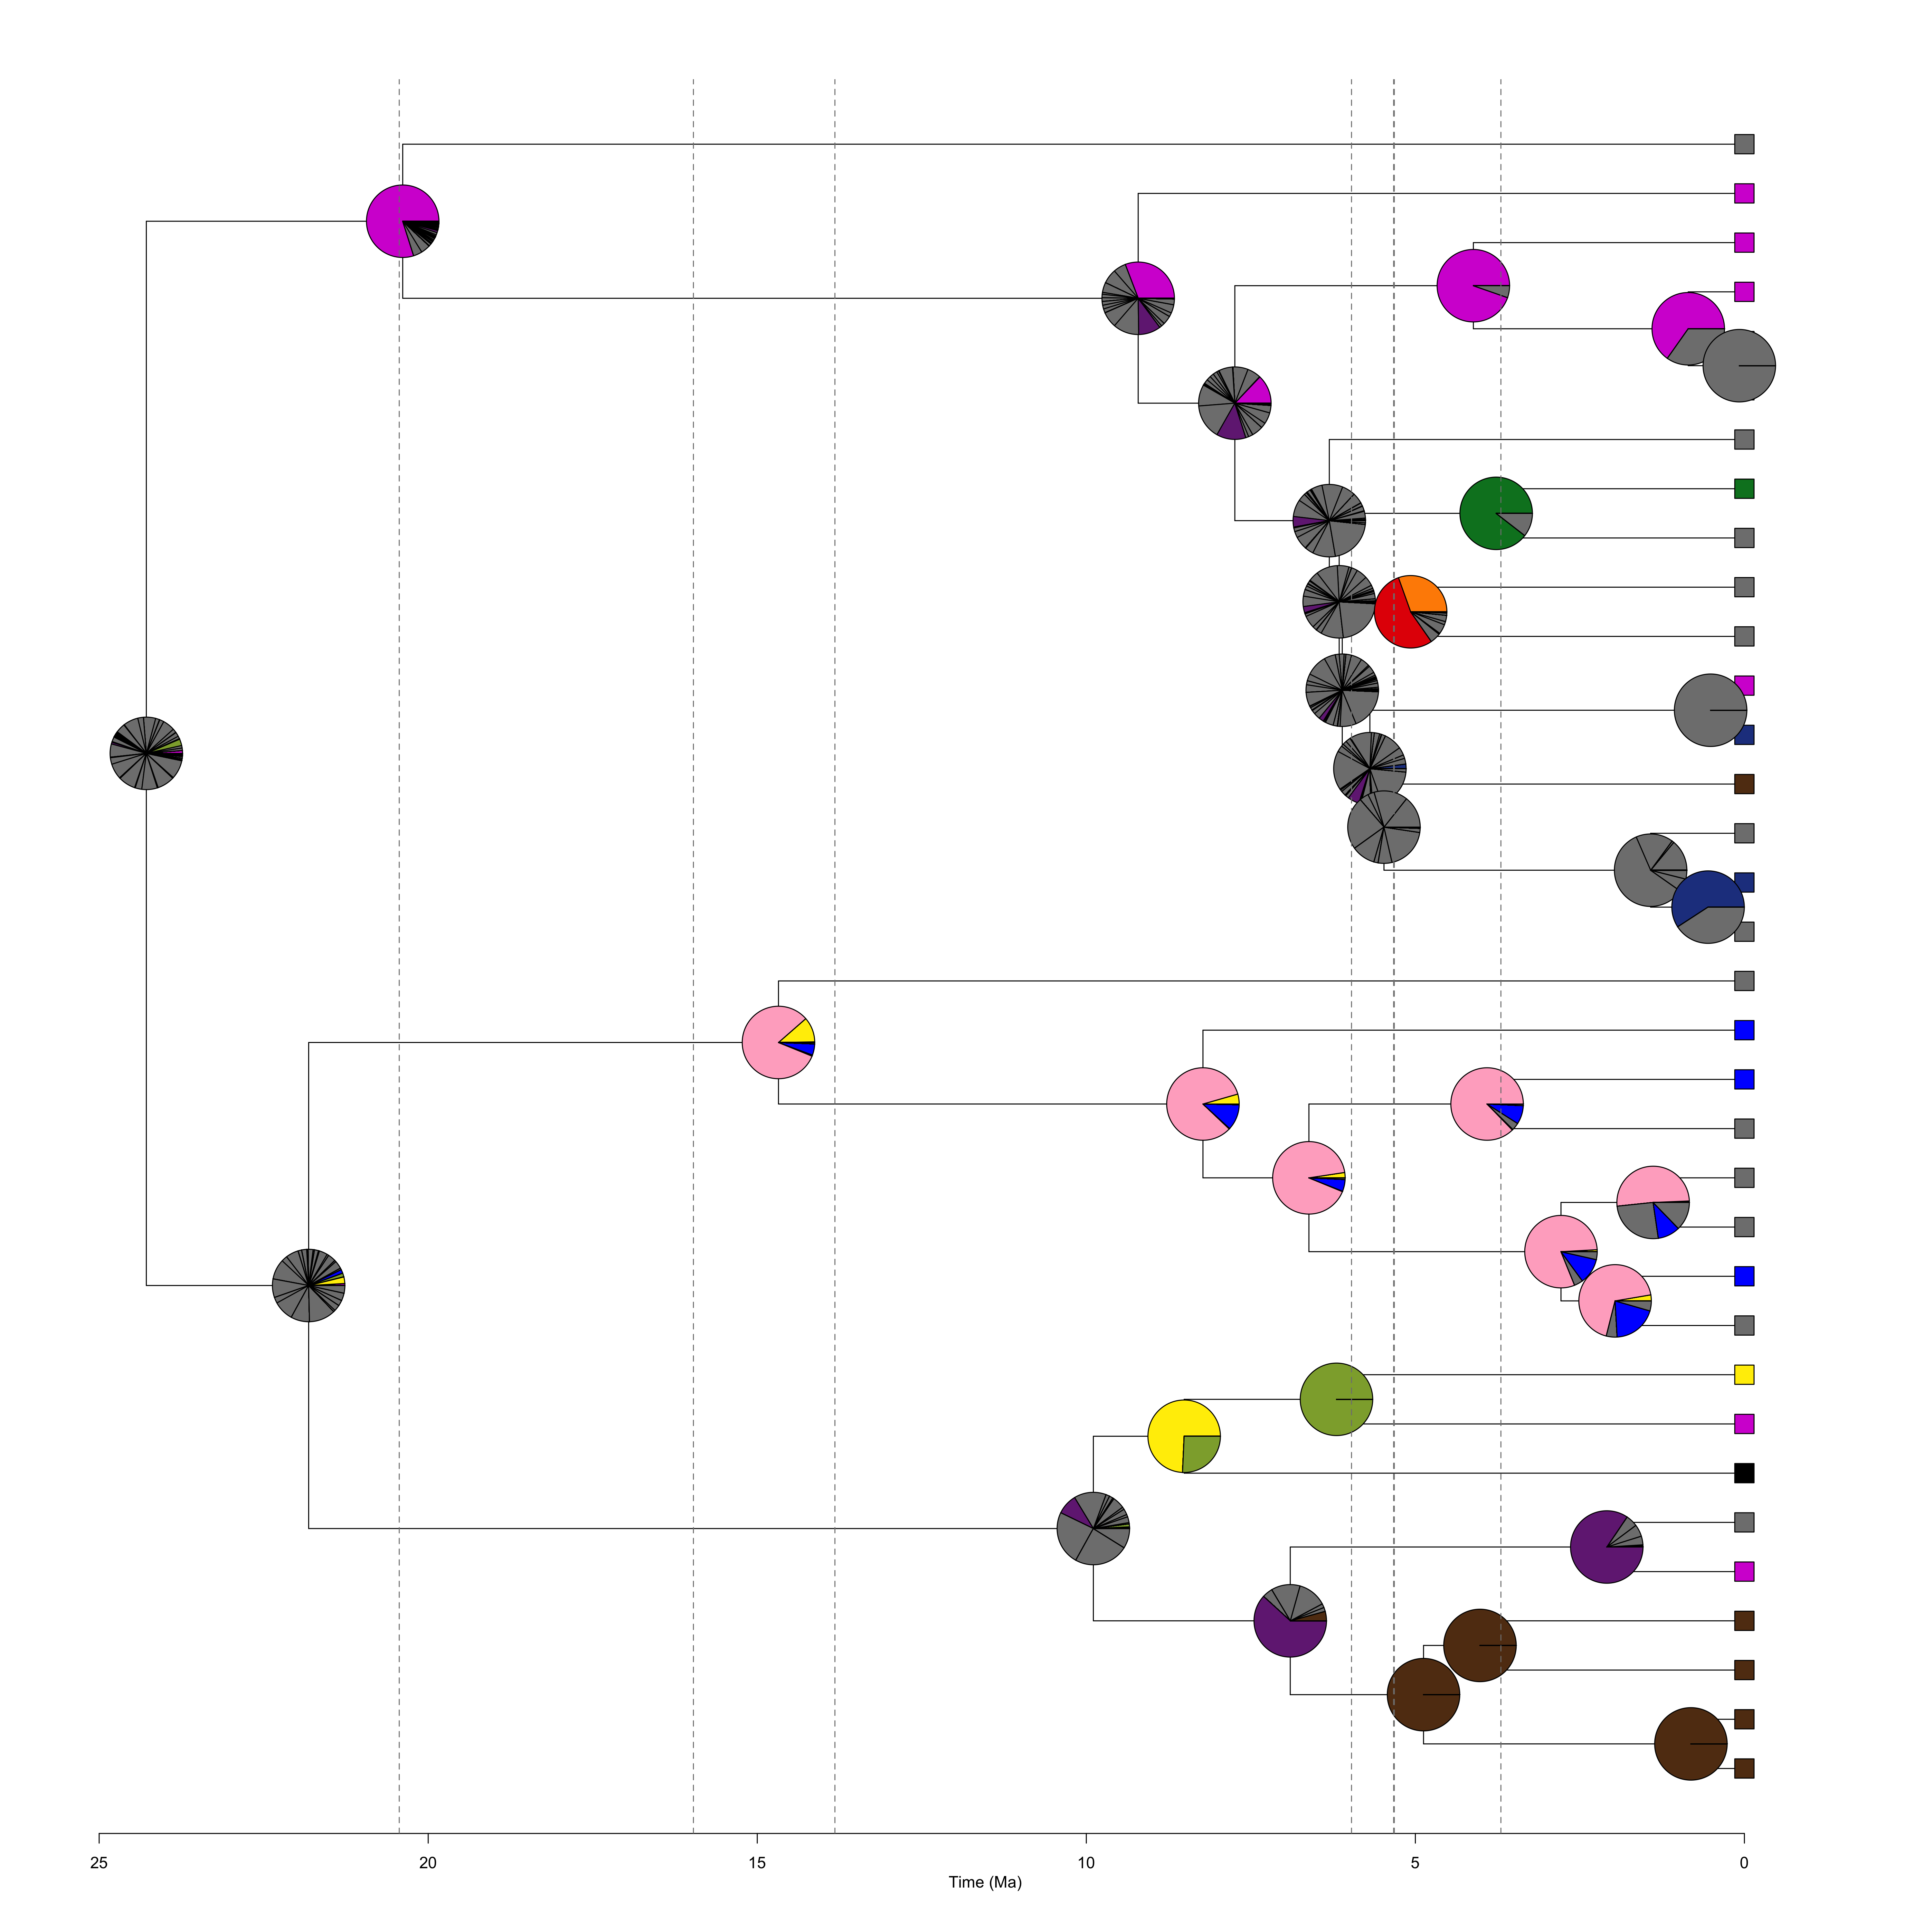
\includegraphics[width = \linewidth]{figures/extant-pinnipeds-DEC-unlikely-pies.png}
%  \caption{extant pinnipeds, DEC model, impossible and unlikely states removed. Nodes show relative probabilities of each state.}
%  \label{fig-extant-dec-pie-unlikely}
%\end{figure} 

% figure
%\begin{figure}[H]
% \centering
%  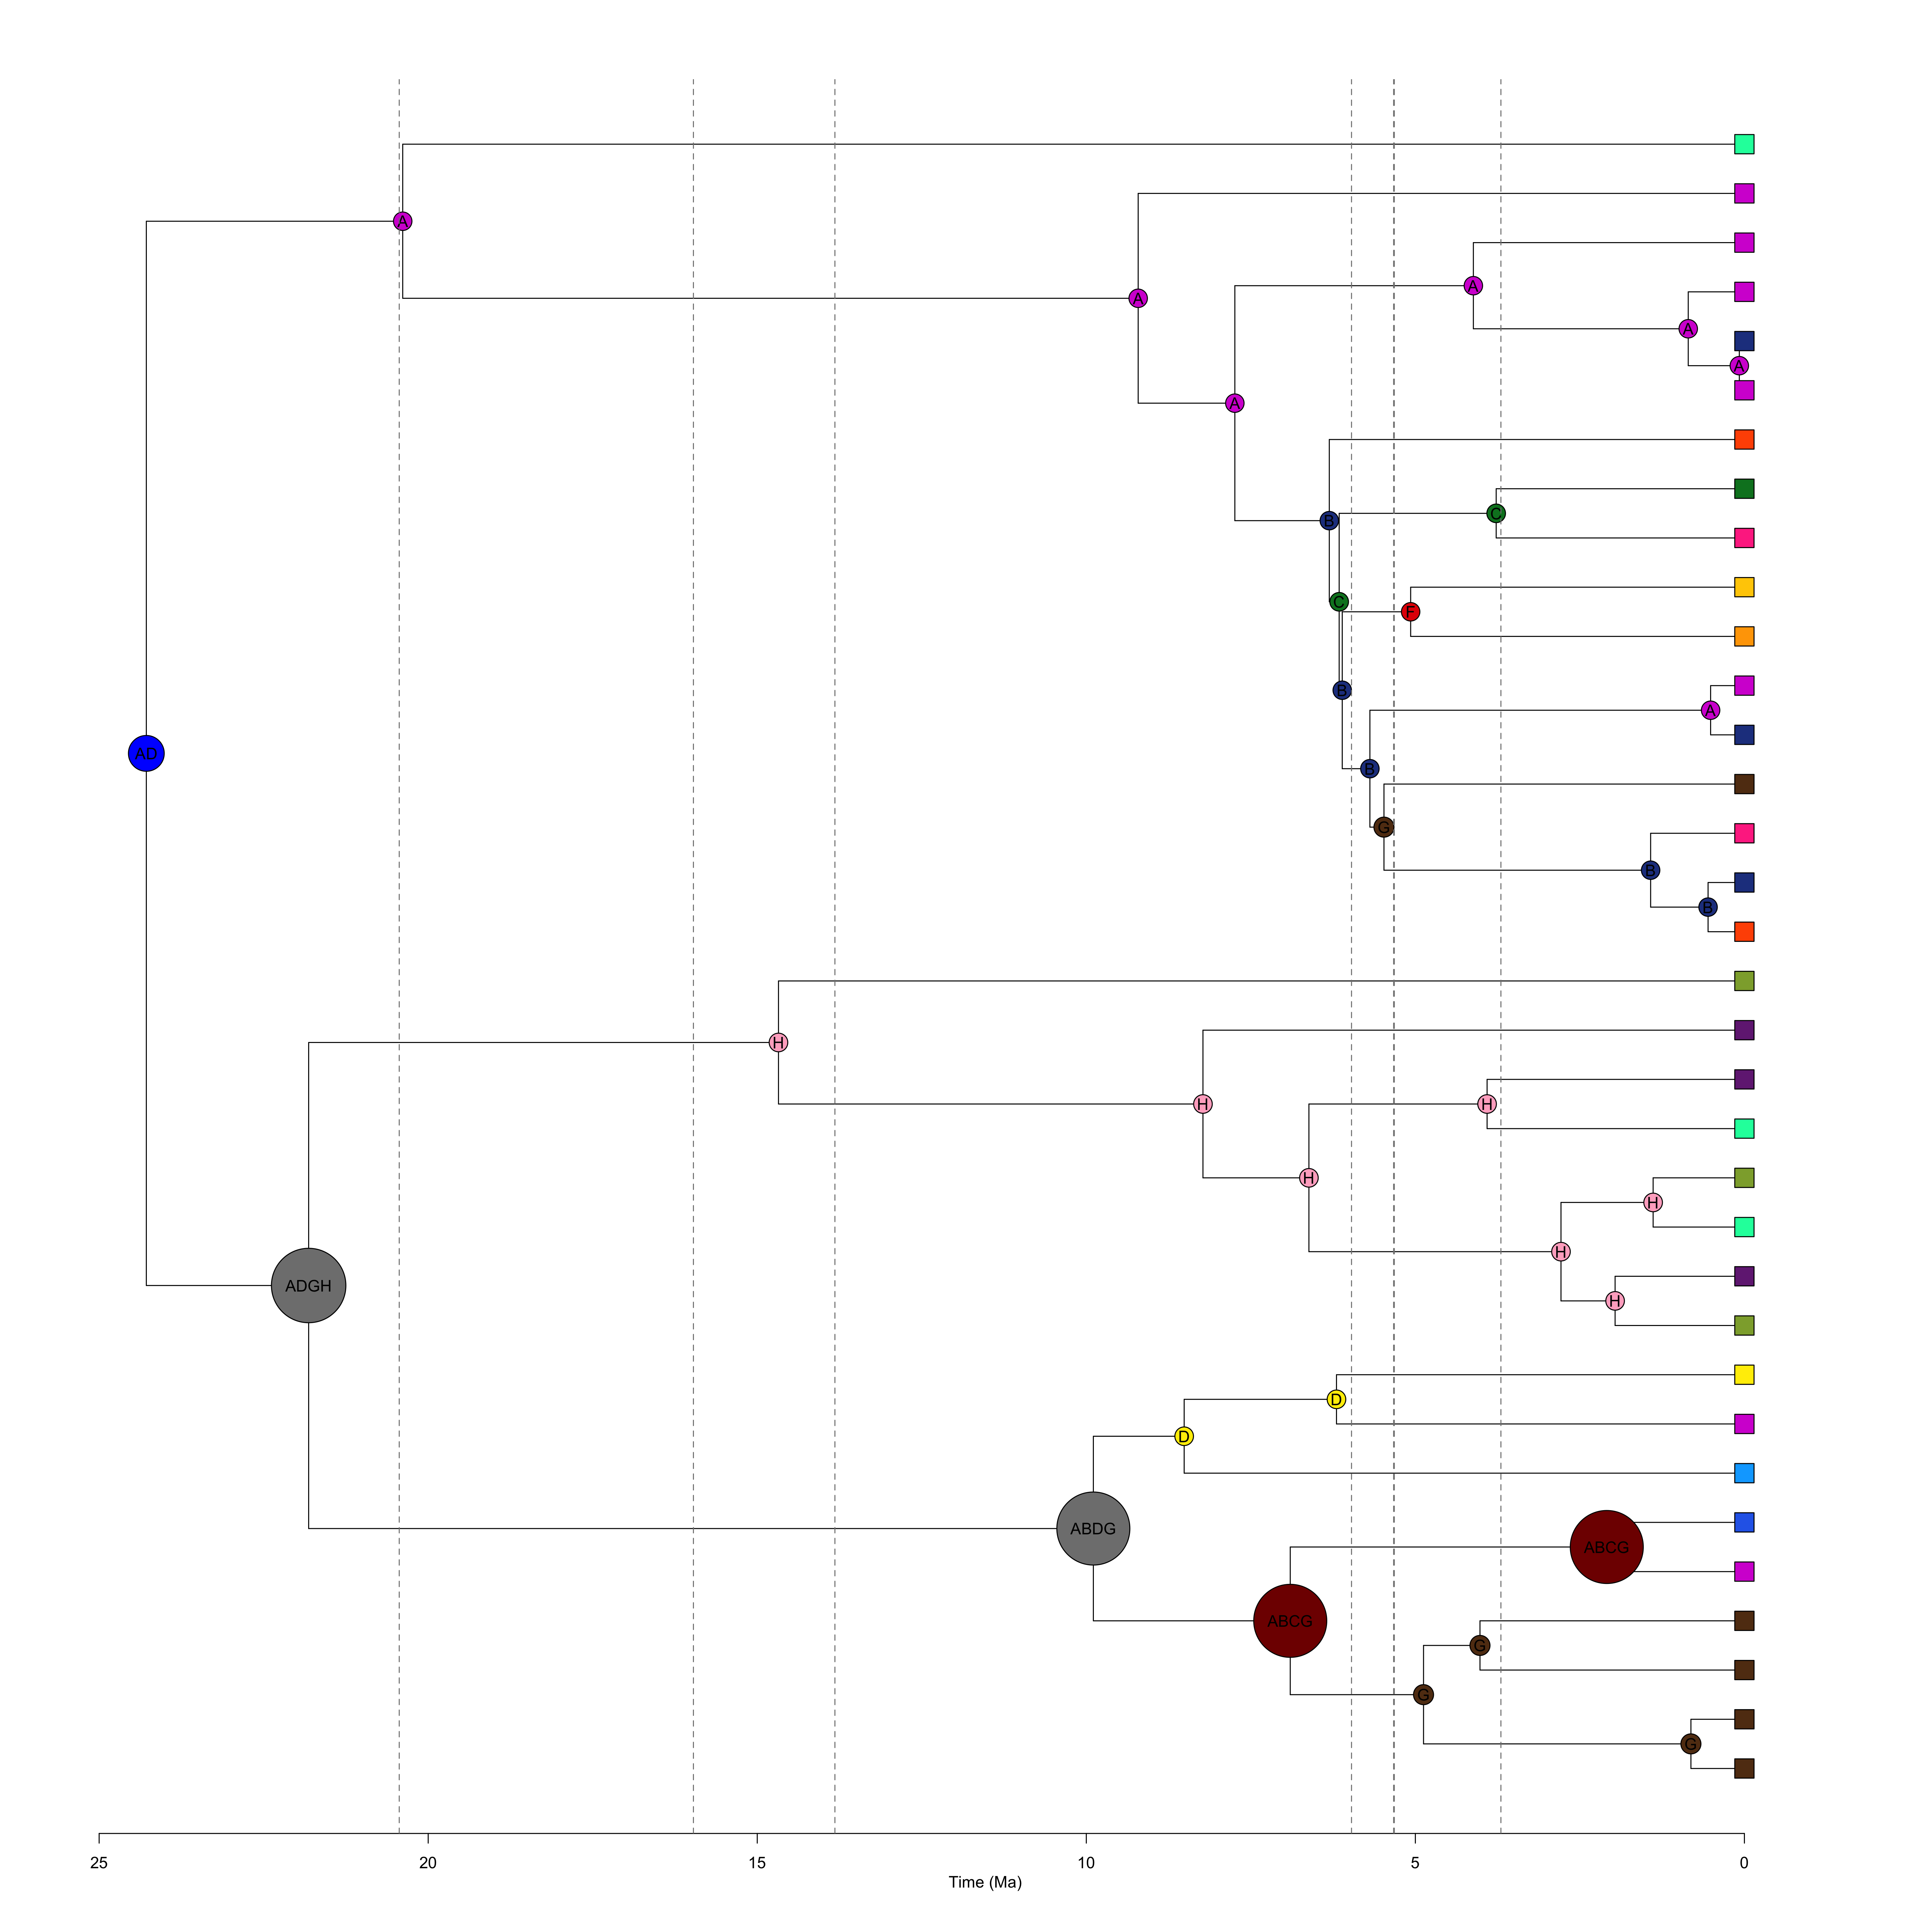
\includegraphics[width = \linewidth]{figures/extant-pinnipeds-DECj-unlikely-MLstates.png}
%  \caption{Extant pinnipeds only, DEC+J model, impossible and unlikely states removed. Nodes show Maximum Likelihood states.}
 % \label{fig-extant-decj-ml-unlikely}
%\end{figure} 

% figure
%\begin{figure}[H]
% \centering
%  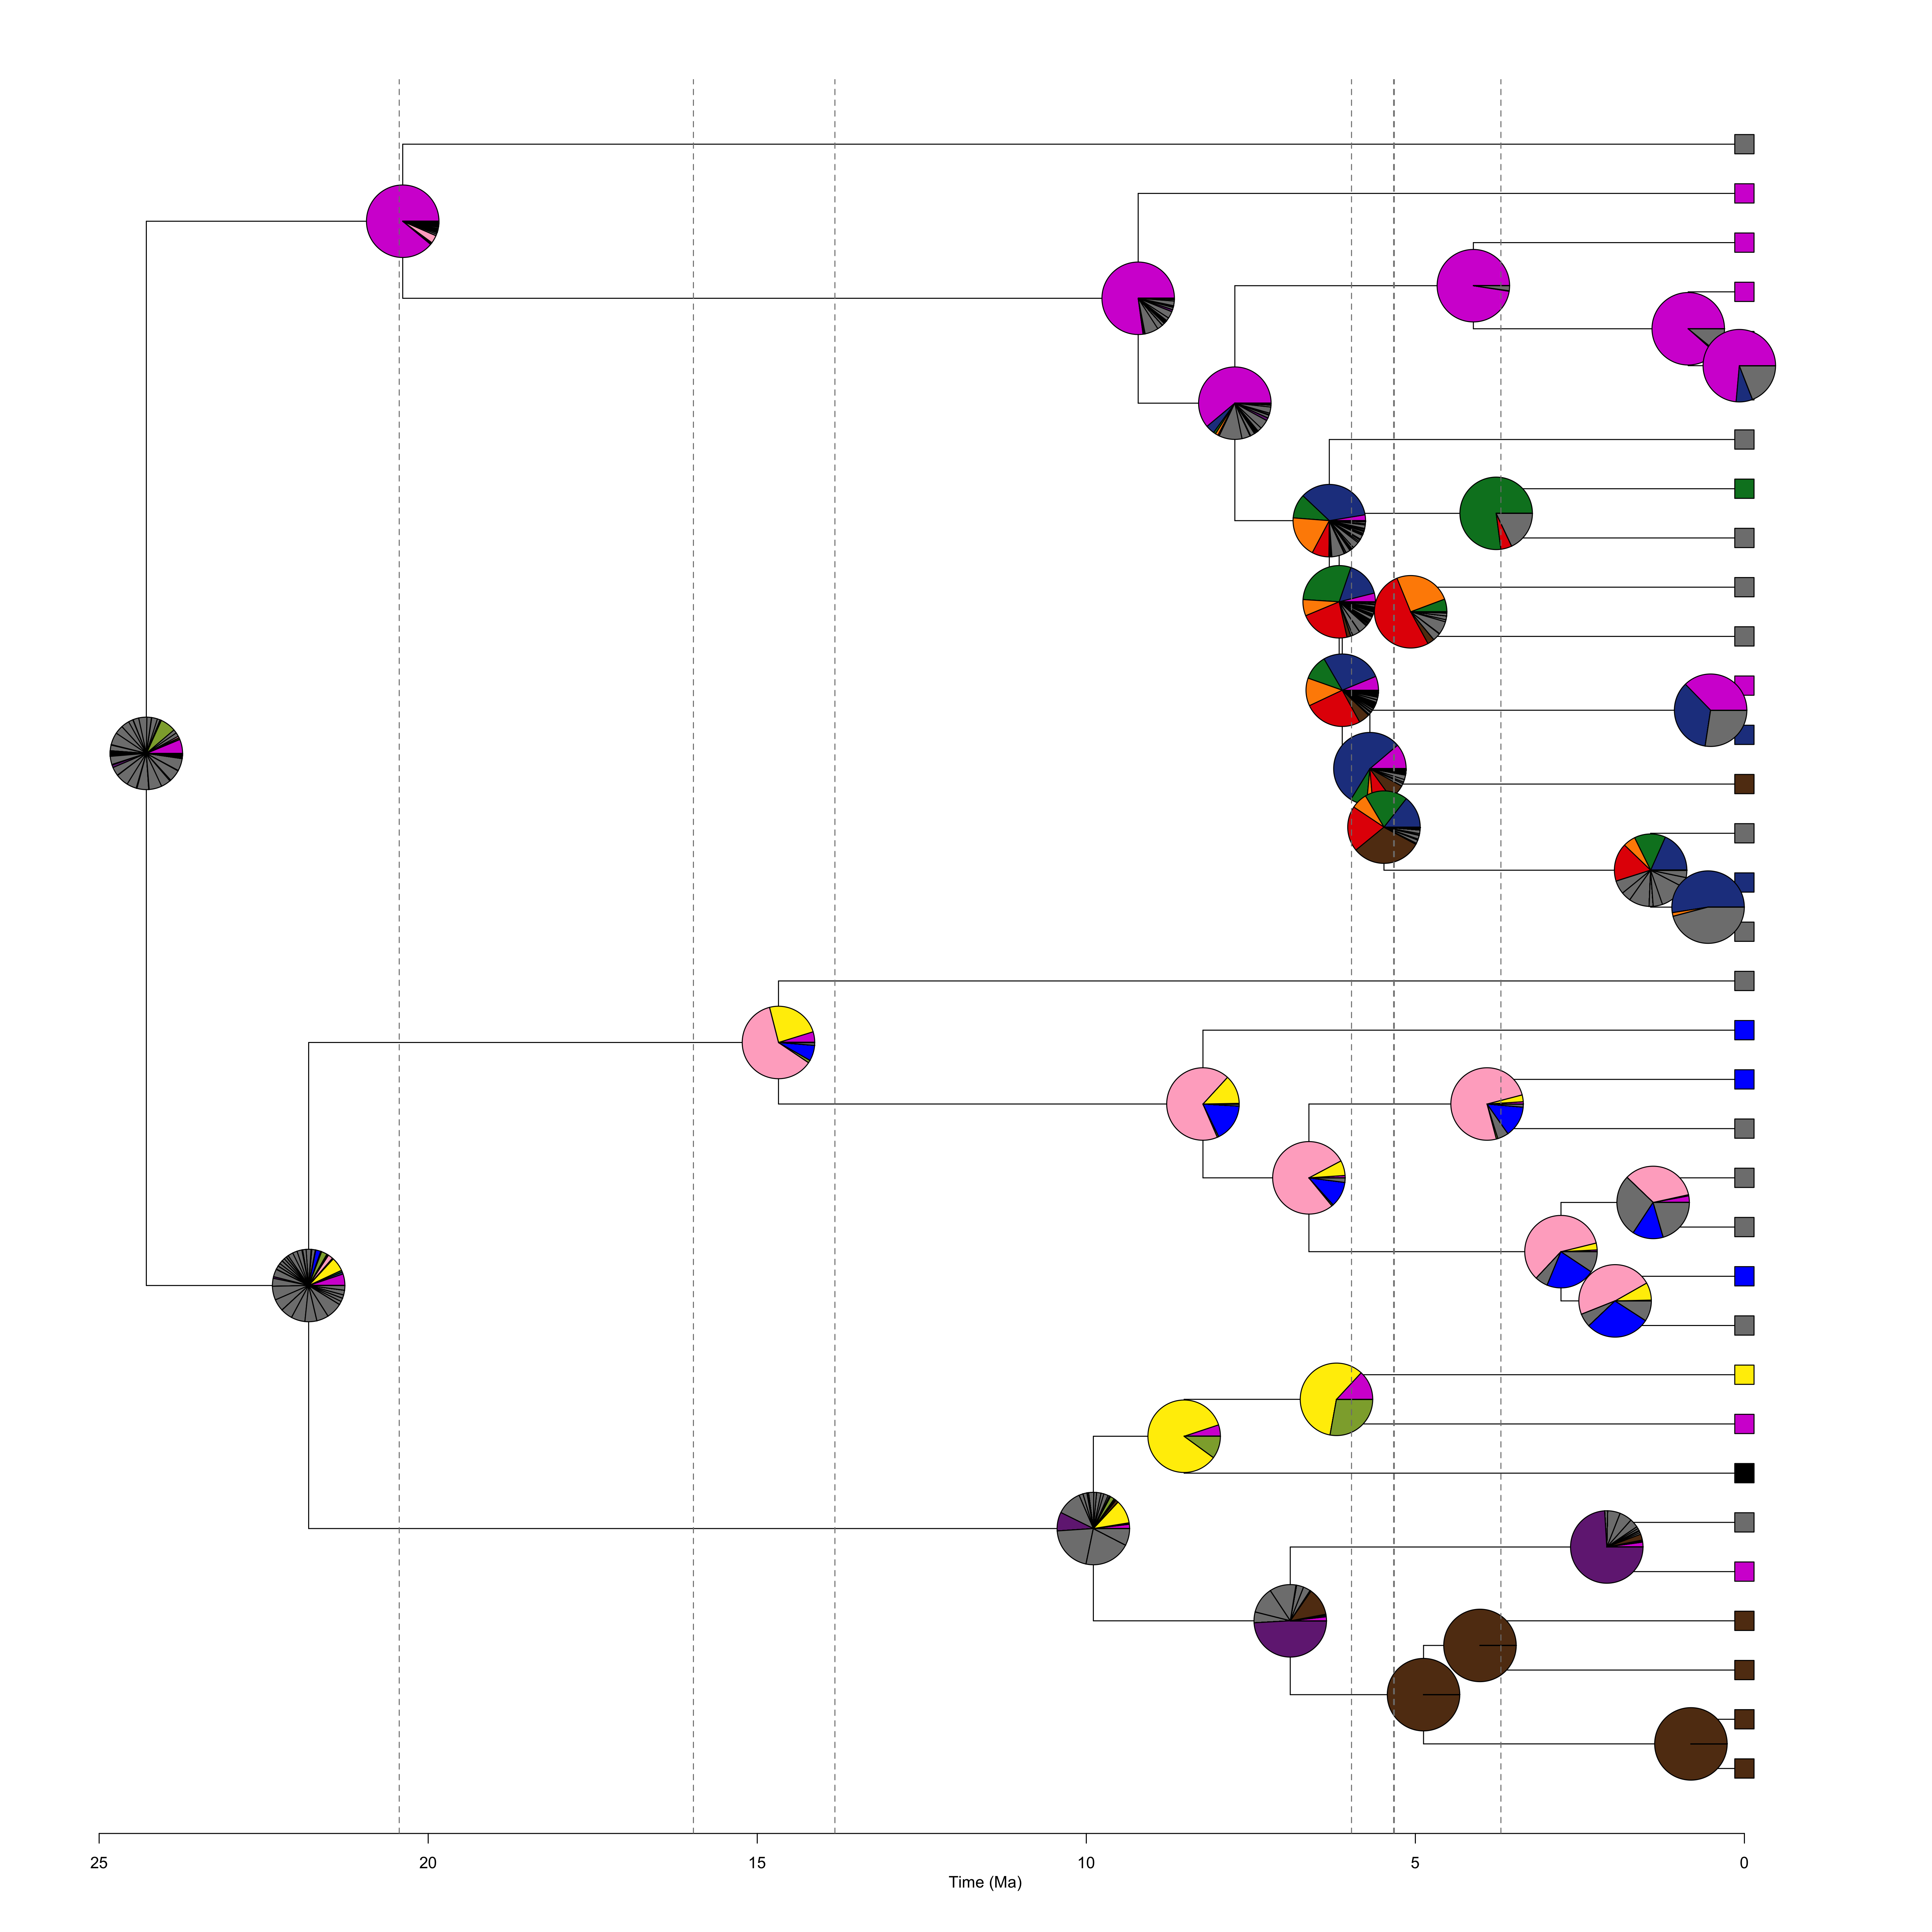
\includegraphics[width = \linewidth]{figures/extant-pinnipeds-DECj-unlikely-pies.png}
% \caption{extant pinnipeds, DEC+J model, impossible and unlikely states removed. Nodes show relative probabilities of each state.}
%  \label{fig-extant-decj-pie-unlikely}
%\end{figure} 

%-------------------------------------------------------------------------------
% Refs
%----------------------------------------
\newpage
\section{Supplementary References}
 
\bibliography{pinnipeds}
\bibliographystyle{vancouver}

\end{document}